\chapter{Evaluation}
kapitelstarttext...
\section{Simulationsaufbau}
Zunächst wird auf den Aufbau des verwendeten Simulators eingegangen, sowie auf die ,in der Simulationen verwendeten, Daten.
\subsection{Simulationsframework und Simulatoren}
Für die Durchführung der Simulation der in Kapitel 3 vorgestellten Methodiken wird die co-Simulations Software Mosaik \footnote{https://mosaik.offis.de/} verwendet. Der Mosiak Simulator wurde speziell für Simulation von Smart Grid-Anwendung entwickelt und eignet sich deswegen hervorragend für die im Zuge dieser Arbeit zu erfüllenden Aufgaben. Der Simulator unterstütz zudem die schnelle Einbing von einem Framework namens PYPOWER. PYPOWER wurde zur Simulation von Stromflüssen entwickelt und ist in der Lage anhand eines Stromnetzes die Ströme der elektrischen Energie zu simulieren. Diese Simulationdes Stromflusses schließt auch den Transportverlust der Niederspannung und den Zusammenhang von Wirk- zu Blindleistung mit ein. Die Art der Integration von PYPOWER in die Mosaik co-Simulations Software, sorgt dafür, dass ein Nutzer PYPOWER nicht außergewöhnlich konfigurieren muss. Ein Stromnetz welches an Mosaik übergeben wird, wird automatisch PYPOWER mitverwenden. Das Stromnetz welches in dieser Arbeit verwendet wird ist ein standardisiertes europäisches Niederspannungsnetz, welches von der IEEE, dem Institut für Elektro- und Elektronikingenieure, für solche Simulation herausgegeben wurde, um Ergebnisse auf einer EU-weiten Ebene vergleichbarer zu machen. Die Methodiken um den Stromfluss im Niederspannungsnetz zu beeinflussen wurden im Kapitel 3 vorgestellt. Dieser Teil des Simulators ist auch der einzige Teil welcher zwischen den verschiedenen Simulationen ausgetauscht wird. Der letzte Baustein welcher für die Simulation benötigt wird, sind die Fahrzeuge, welche geladen werden sollen. Dieser Simulator ist in der Lage anhand der aus dem Netz abgerufen Leistung und der Zeit zu bestimmen, wie sich die Fahrzeugparameter verändern. Die verschiedenen Teile des Simulators benötigen an manchen Stellen Daten von anderen Teilen des Simulators. Die Methodiken, welche in dieser Arbeit entwickelt wurden setzen an den Anschlusspunkten des Niederspannungsnetzes für Privatverbraucher an. Über diese Anschlusspunkte wird unter anderem die Leistung bezogen, welche für das laden der mit diesem Anschlusspunkt verbunden Elektrofahrzeuge verwendet wird. Die aktuell verwendete Methodik erhält vom jeweiligen Anschlusspunkt die aktuell anliegende Spannung. Die mit dem jeweiligen Anschlusspunkt verbunden Elektrofahrzeuge, teilen der Methodik die Ankunftszeit, den Abfahrtszeitunkt, die aktuell möglich Stromstärke beim Laden, sowie den aktuellen Ladestand mit. Das jeweilige Elektrofahrzeug bezieht dann die von der Methodik berechnete mögliche Ladeleistung aus dem Netz, teilt diesem also die Höhe der bezogenen Leistung mit. Die Transformatorlast wird über ein Broadcastsystem vom Transformator aus verteilt, Die Teilnehmeranzahl kann von jeder Methodik, anhand der erhaltenen Nachrichten bestimmt werden. Diese Nachrichten wurden wiederrum von anderen Teilnehmer versandt.\\
\begin{figure}[htb]
\centering
	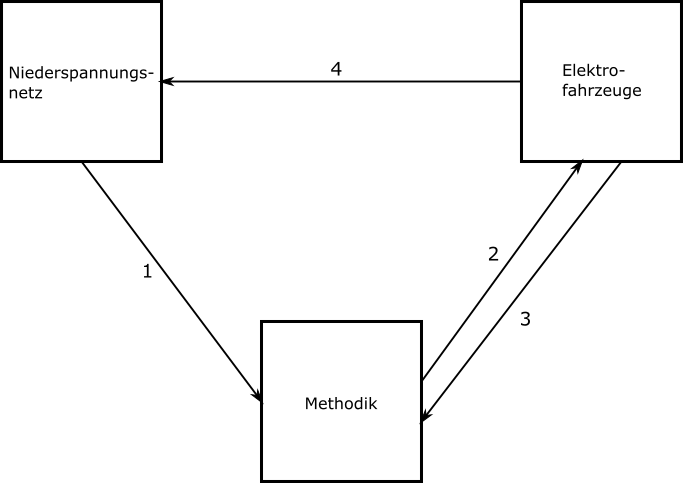
\includegraphics[width=0.5\textwidth]{img/SimAufbau1.png}
	\caption{Schnittstellen zwischen den Teilen des Simulators}
	\label{Abb_SimAufbau}
\end{figure}

In der Abbildung \ref{Abb_SimAufbau} wird ersichtlich wer welche Daten an wen weitergibt. Die mit der eins markierte Verbindung stellt die Weitergabe von Daten  vom Niederspannungsnetz an die aktuelle verwendete Methodik dar. Dabei wird die aktuell am Anschlusspunkt gemessene Spannung weitergegeben. Die zwei mit zwei und drei markierten Übergänge verdeutlichen den Datenaustausch zwischen der verwendeten Methodik und dem angeschlossen Elektrofahrzeug. Das Elektrofahrzeug sendet die Ankunftszeit, die Abfahrtszeit, die aktuell maximal mögliche Stromstärke und den Ladezustand an die Methodik und erhält im Gegenzug die aktuelle Höhe der aus dem Netz beziehbaren Leistung. Über die Verbindung, welche mit 4 markiert ist, wird dem Netz von Elektrofahrzeug mitgeteilt, welche Leistung aktuell aus dem Netz bezogen wird.
\subsection{Annahmen und verwendete Daten}
Im Zuge dieser Arbeit wird eine nicht unerhebliche Menge an Daten verarbeitet. Die Mehrheit dieser Daten steht in Zusammenhang mit den Elektrofahrzeugen. Die Daten die diese für die Simulation zur Verfügung stellen, wurden vom Deutschem Zentrum für Luft – und Raumfahrt erhoben. Diese Erhebung fand im Zuge einer Mobilitätsstudie statt. Es wurden Teilnehmer für diese Studie aus der Bevölkerung ausgewählt, welche dann ihr Mobilitätsverhalten dokumentiert haben. Diese Mobilitätsverhalten dienen als Grundlage für die Daten der verwendeten Elektrofahrzeuge. Durch die Auswertung dieser Daten wurden Ankunfts- und Abfahrtszeiten, sowie die jeweils gefahrene Wegstrecke bestimmt. Durch die Länge der Wegstrecke kann bestimmt werden wie viel des Ladezustandes auf dieser Strecke verbraucht wird und somit auch der Ladestand bei Ankunft an der Ladestation.\\
Es werden für die Simulationen auch einige Annahmen getroffen. Der Kapazität der Batterie, in welcher die elektrische Energie der Elektrofahrzeuge gespeichert wird, wird auf 36253,11 Wh festgelegt. Dieser Wert wurde durch Auswertung zweier Statistiken ermittelt, welche die meistzugelassen Elektrofahrzeuge in Deutschland beinhalteten und die Batteriekapazität pro Modell. Durch die Verwendung dieser Statistiken wurde eine durchschnittliche Batteriekapazität der Elektrofahrzeuge in Deutschland ermittelt. Dieser Mittelwert stellt einen Kompromiss zu einer individuellen Batteriekapazität dar, stellt allerdings auch sicher vergleichbare Ergebnisse zu erhalten. Die Norm DIN EN 50150 setzt die Normspannung im Deutschem Stromnetz auf 230 Volt, daher wird dieser auch in dieser Arbeit verwendet. Die maximale Trafolast wurde durch eine Simulation ohne Aktivität von Elektrofahrzeugen ermittelt. Die, in dieser Simulation gemessene, Transformatorlast wurde verdoppelt. Diese Verdopplung soll die Belastung des Transformators so gering wie möglich halten, den Ladevorgängen aber dennoch die Möglichkeit bieten auch Leistung abzurufen. Eine weitere Annahme ist die maximale Anzahl an Elektrofahrzeugen, hierbei wurde davon ausgegangen, das ein jeder Haushalt im Niederspannungsnetz über exakt zwei Elektrofahrzeuge verfügt, welche mithilfe eine 22kW Ladegeräts geladen werden. Diese Annahme geht aus Statistiken eines Bundesamtes zurück, welche aussagt, das in ländlich geprägten Gebieten vermehrt größere Haushaltemit zwei oder mehr Personen auftreten. Aus Gründer der Normalisierung zwischen den Anschlusspunkten ans Niederspannungsnetz, wird daher immer von zwei Fahrzeugen je Anschlusspunkt ausgegangen. bei dem in dieser Arbeit verwendtem Netz dem IEEE906 gibt es 55 Anschlüsse für Haushalte, folglich wird von 110 Elektrofahrzeugen ausgegangen.

\section{Simulationsergebnisse}
Die Ergebnisse der durchlaufenen Simulationen werden zunächst aufgeteilt auf die verschiedenen Methodiken vorgestellt. Eingegangen wird auf die verursachte Trafolast, die Spannungen, aufgetretene und behandelte Kollisionen, sowie die Qualitätserfahrungen und die Fairness zwischen den Ladevorgängen. 
\subsection{VDE-Controller}
\label{chap_VDE}
Die Verwendung des VDE-Spannungscontrollers (\ref{capBody:VDE}) wurde über einen Zeitraum von einer Woche hinweg simuliert, dargestellt werden die Ergebnisse eines einzelnen Werktages. Ein Werktag wurde gewählt, da die Mehrheit der simulierten Tage ein Werktag ist. Dargestellt wird die Transformatorlast, die minimalen Werte der Spannung sowie die Anzahl der Teilnehmer, welche Leistung aus dem Netz beziehen. 
\begin{figure}
	\begin{subfigure}{\linewidth}
		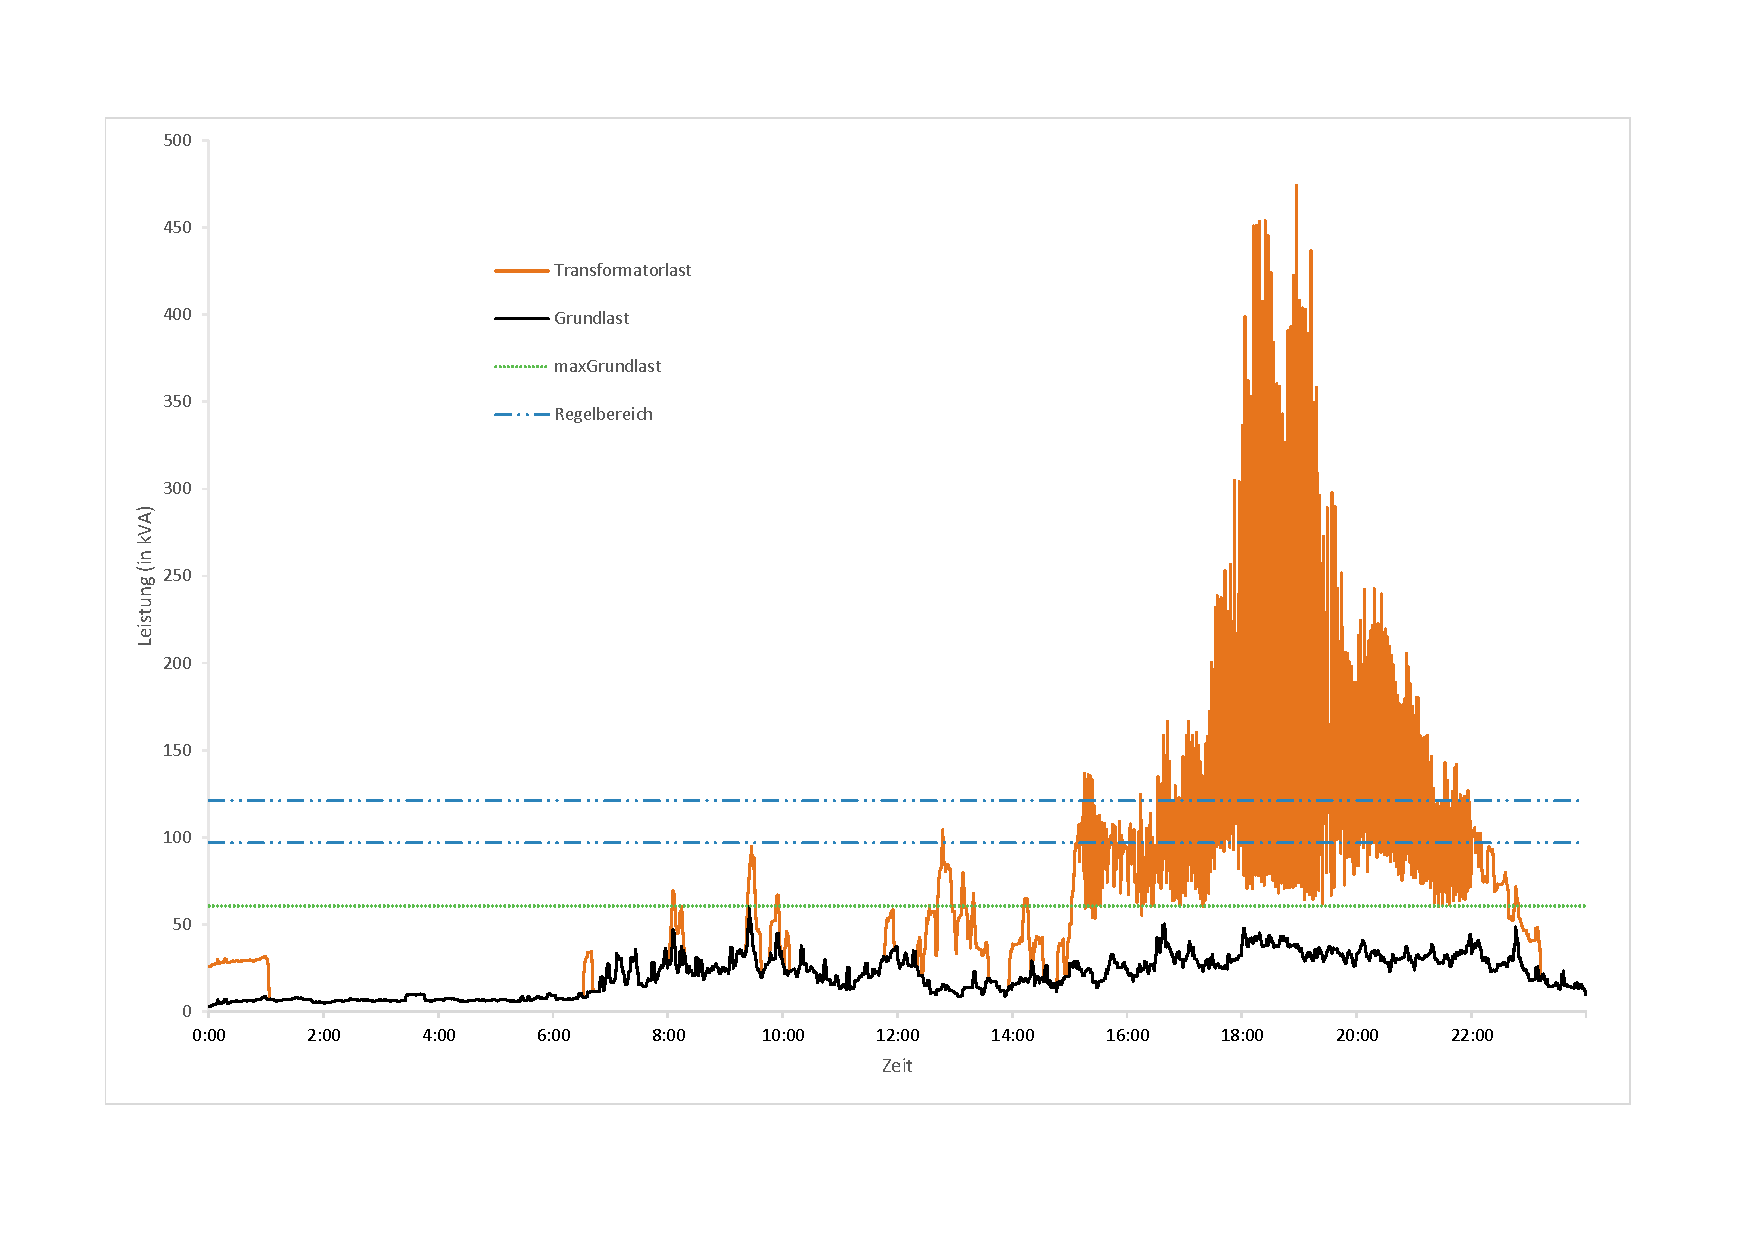
\includegraphics[scale=0.5]{img/VDE_tau/TrafoLast8.pdf}
		\caption{Transformatorlast bei Verwendung des VDE Spannungs-Controllers}
		\label{Abb_VDEtauTrafoLast}
	\end{subfigure}
	\begin{subfigure}{\linewidth}
		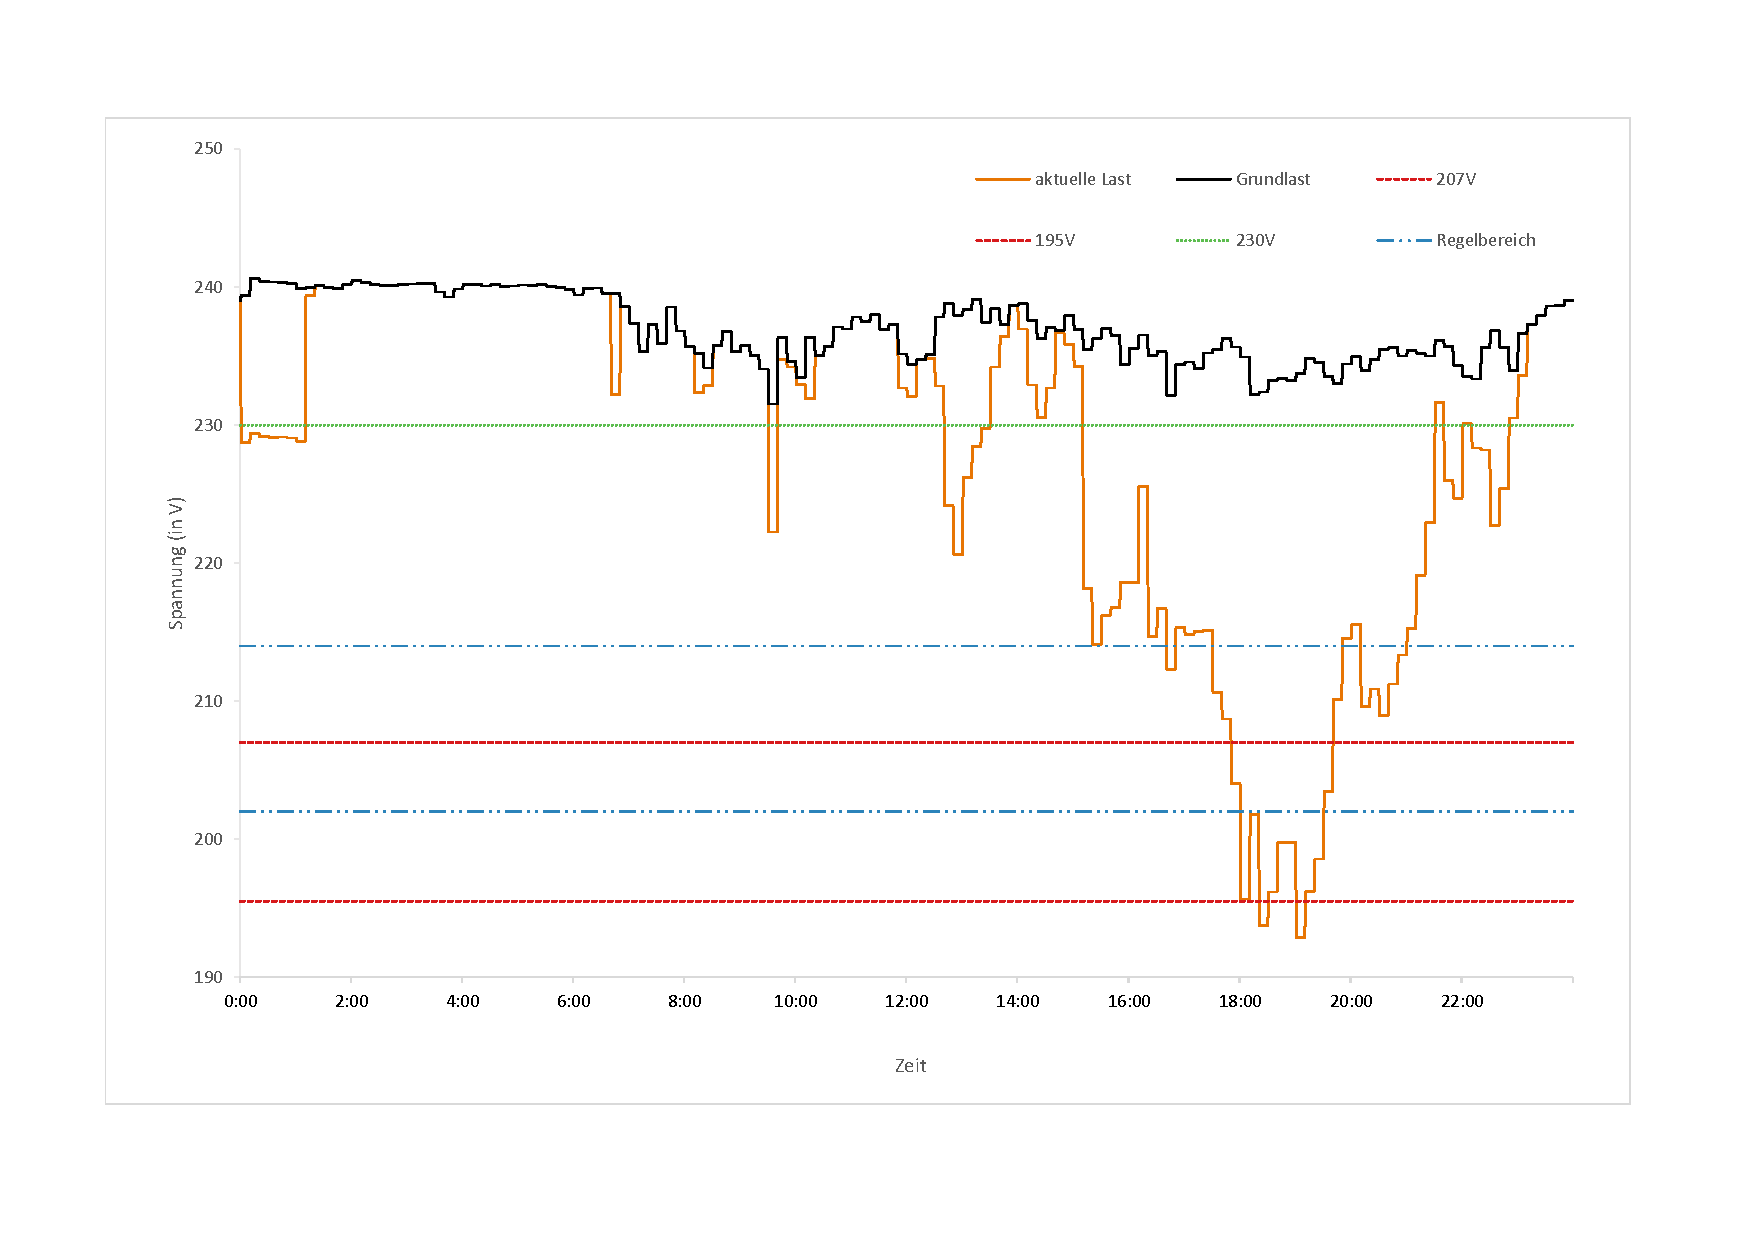
\includegraphics[scale=0.5]{img/VDE_tau/Voltage2.pdf}
		\caption{Spannungsverlauf mit 10 Minuten Mittelwerten bei Verwendung des VDE Spannungs-Controllers}
		\label{Abb_VDEtauSpannung10m}
	\end{subfigure}
	\caption{this needed}
\end{figure}

In der Abbildung \ref{Abb_VDEtauTrafoLast} ist die vom Transformator ans Niederspannungsnetz abgegeben Scheinleistung in kVA über den Verlauf eines Tages abgebildet. Der Regelbereich des Controllers ist im Falle der Transformatorlast nicht relevant, der VDE Controller lediglich die Spannung berücksichtigt. \\
In der Abbildung \ref{Abb_VDEtauSpannung10m} ist der Verlauf der minimalen Spannung über das gesamte Niederspannungsnetz hinweg aufgezeichnet. Bei den dargestellten Werten handelt es sich nicht um minutengenaue Messwerte, sondern um die Mittelwerte von 10 Minuten Intervallen. Diese Intervalle wurden gewählt um die Erfüllung der Norm DIN EN 50160 zu bestimmen. Die Norm befasst sich allerdings mit der Spannung an einzelnen Anschlusspunkten, dargestellt werden allerdings Werte aus dem gesamten Niederspannungsnetz, somit lässt sich anhand des Graphen nur bestimmen, ob die Norm von allen Anschlusspunkten eingehalten wurde. Bei einem sichtbaren Verstoß gegen die Norm, lässt sich nur das Vorhandensein eines einzelnen Verstoßes ableiten, da nur minimal Werte dargestellt werden. Ob zeitgleich noch andere Anschlusspunkte gegen die Norm verstoßen haben ist anhand des Graphens nicht feststellbar.
\begin{figure}[htb]
	\centering
	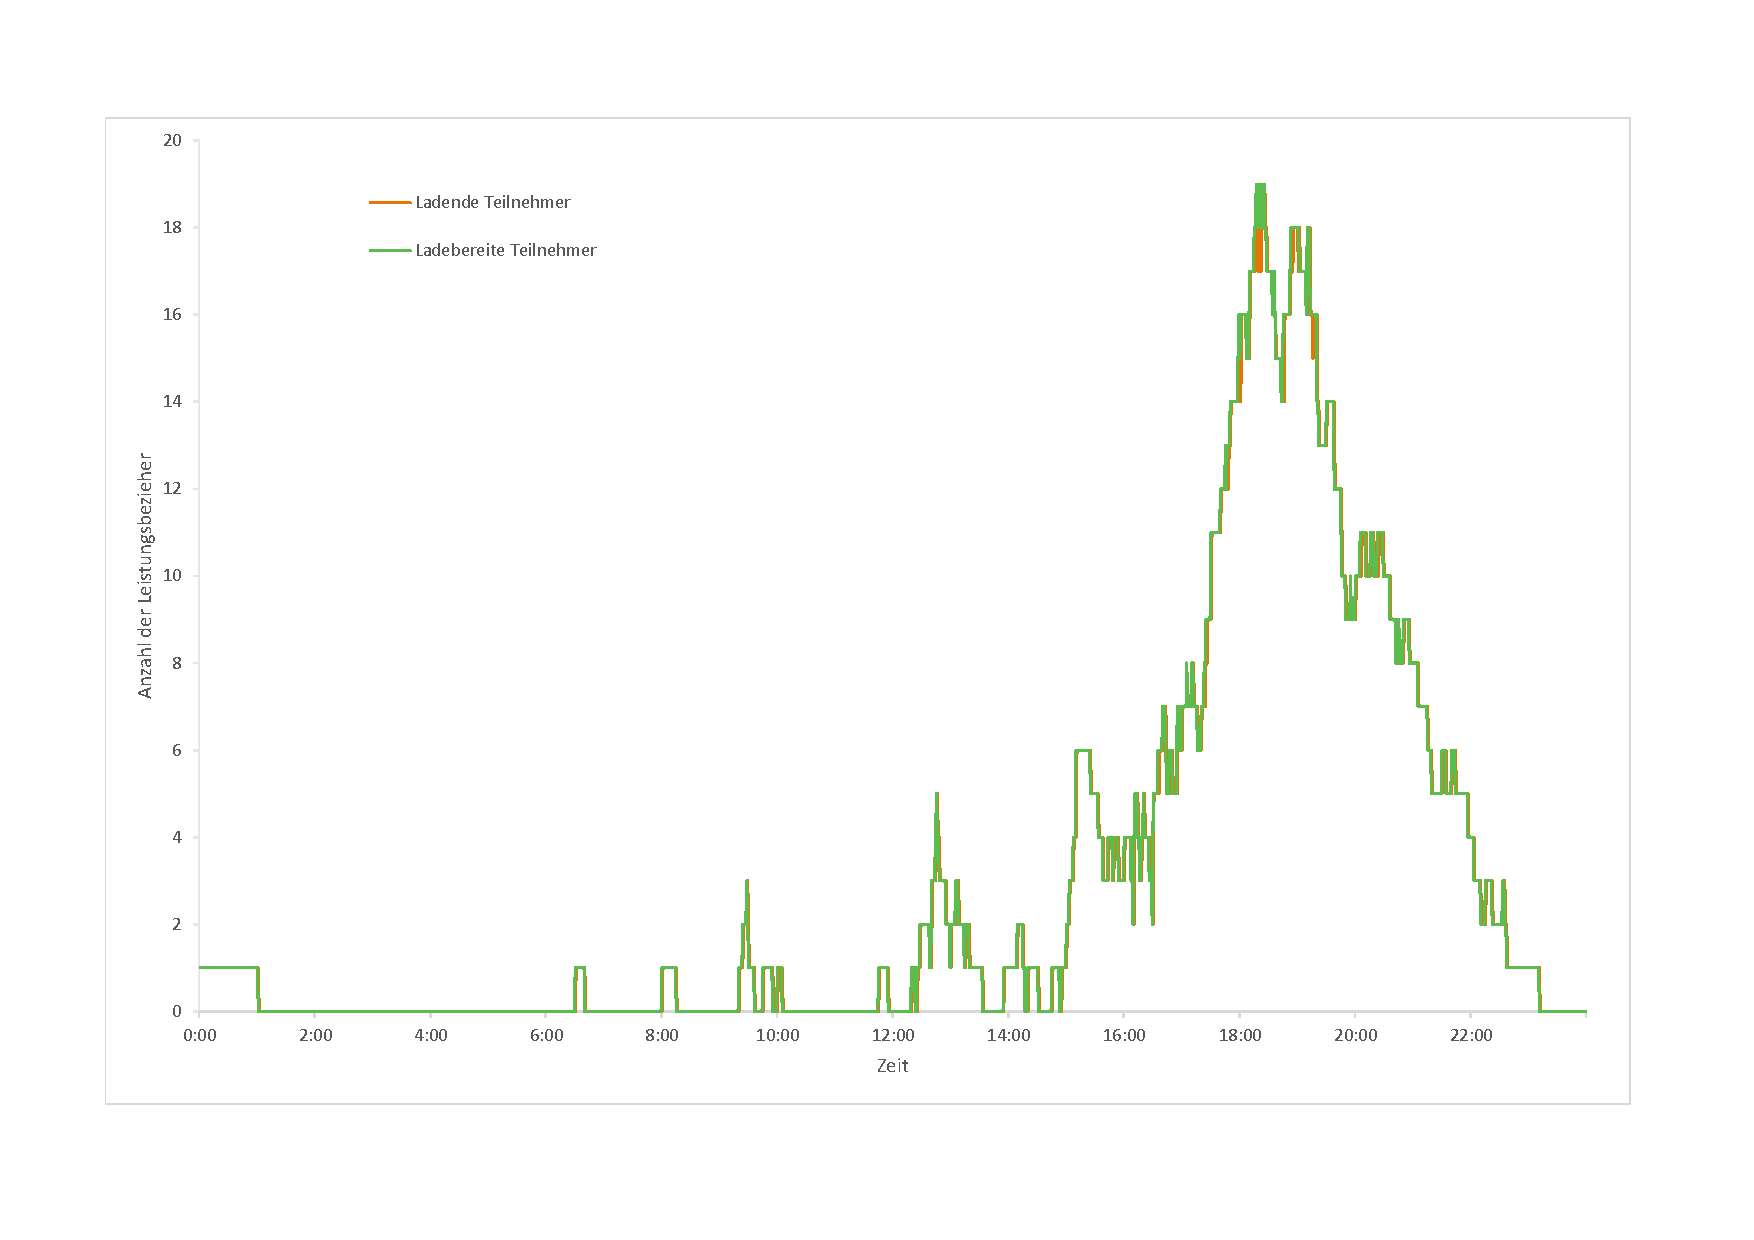
\includegraphics[scale=0.5]{img/VDE_tau/Teilnehmer2.pdf}
	\caption{Teilnehmeranzahl bei Verwendung des VDE Spannungs-Controllers}
	\label{Abb_VDEtauTeilnehmer}
\end{figure}
In der Abbildung \ref{Abb_VDEtauTeilnehmer} ist die Anzahl an ladebereiten und tatsächlich ladenden Teilnehmern abgebildet. Ein Abstand zwischen den beiden Kurven weist daraufhin, dass es ladebereite Teilnehmer gibt, welche aber nicht laden. Die große Ähnlichkeit der beiden Kurven und die wenigen sichtbaren Unterschiede zeigt das diese Menge an Teilnehmern bei dieser Methode möglich ist für gleichzeitiges laden.\\
Bis etwa 16:00 steigt die bezogene Leistung am Transformator mehrmals über die Grundlast hinaus an, diese Anstiege decken sich mit einer Zunahme an Teilnehmer und sich auch an der fallenden Spannungskurve erkennbar. Die Belastungen bis zu diesem Zeitpunkt sind allerdings nicht hoch genug, dass die Spannung den Regelbereich des Spannungscontrollers erreicht. Um etwa 16:00 fällt die Spannung bis zum Beginn des Regelbereiches ab, steigt dann aber wieder an, was sich auf eine sinkende Teilnehmeranzahl zurückführen lässt. Nach 16:00 steigt die Anzahl der Teilnehmer innerhalb zweier Stunden stark an, von etwa 4 auf bis zu 18 Teilnehmer. Dieser Anstieg an Teilnehmern führt auch zu einer gesteigerten Menge an bezogener Ladeleistung. In derselben Zeit fällt auch die Spannung ab, zunächst nur bis in den Regelbereich hinein. Ab etwa 18:00 liegt die minimal gemessene Spannung unterhalb des Regelbereiches des Spannungscontrollers, etwa zwei Stunden lang werden Spannungen unterhalb des Regelbereiches gemessen. Erst als die Teilnehmerzahl ab 20:00 sinkt und damit auch die Transformatorlast wieder zurückgeht, steigt die Spannung wieder an. Der Abfall der Spannung unterhalb des Regelbereiches zeigt an, das der Spannungscontroller nicht mehr ordentlich arbeiten und nicht in der Lage ist die Spannung auf einem ausreichenden Niveau zu halten. Der Wert der Spannung der 10 Minuten Intervalle fällt auf bis zu 184,60 V ab, da dies weniger als 15 \% der Normspannung entspricht, wird die Norm DIN EN 50160 nicht erfüllt. An der Kurve der Transformatorlast lässt sich erkennen, dass der Spannungscontroller zwar arbeitet, die vorgenommen Regelungen allerdings in einer stark schwankenden Transformatorlast resultieren. \\

Die hier vorgestellte Methodik reagiert auf keine Art von Kollision, dennoch wurde die Anzahl von Situationen erfasst, in denen Kollisionen aufgetreten wären. Hierbei gibt es zu beachten, dass der Simulationszeitraum 10080 Schritte umfasst, welche von jedem der 110 betrachteten Fahrzeuge durchlaufen werden. Dies bedeutet es werden 1108800 Situationen betrachtet. In 0,13 \% davon ist eine Spannungskollision aufgetreten und in 0,15 \% davon ist eine Transformatorkollision aufgetreten. In insgesamt 0,15 \% der Fälle, also 5615 Situationen, trat eine Art von Kollisionen auf. Diese Arten der Kollisionen beinhalten eine reine Spannungskollision, eine reine Transformatorkollision, sowie eine Spannungskollision und Transformatorkollision, welche zeitgleich auftreten. \\

Innerhalb des Simulation Zeitraumes werden insgesamt 557 Ladeservices gestartet, von denen alle erfolgreich abgeschlossen wurden. Dies bedeutet, dass ein jedes Fahrzeug beim Verlassen der Ladestation einen Ladezustand von 100 \% aufwies. Beim Start eines Ladeservices lag der durchschnittliche Ladestand bei etwa 85 \%, schon nach etwa 40 \% des Ladeservices liegt der durchschnittliche Ladestand bei fast 100 \% mit einer Standardabweichung von lediglich 0,8 \%. Der schnelle Anstieg des durchschnittlichen Ladestandes zeigt das die Fahrzeuge sehr früh und gleichmäßig mit hohen Mengen an Energie versorgt werden. \\
\begin{figure}
	\begin{subfigure}{0.49\linewidth}
		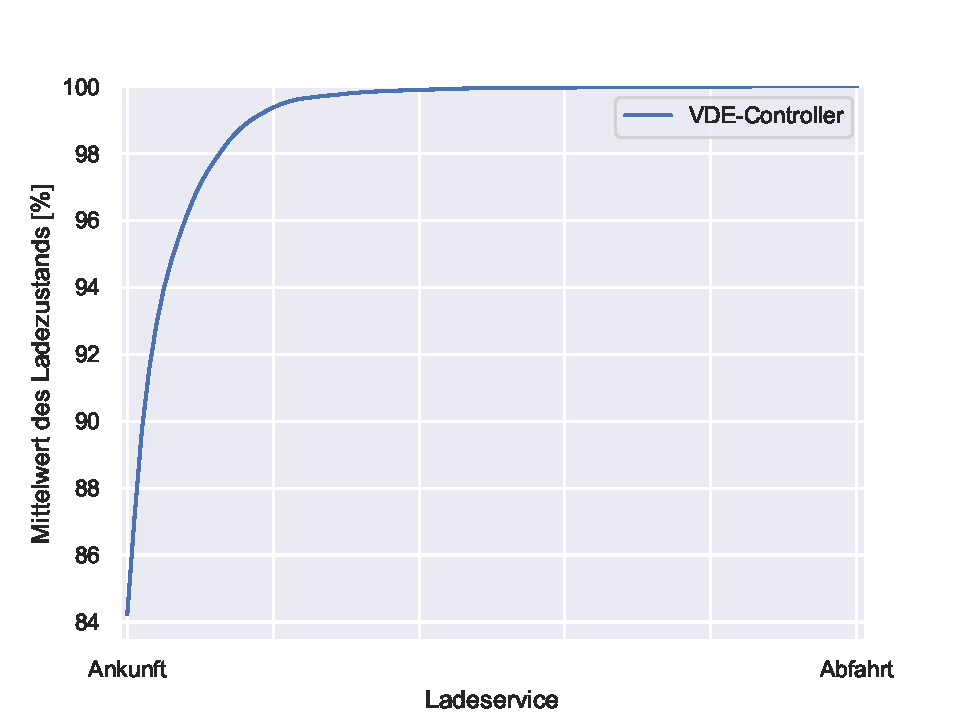
\includegraphics[width=\linewidth]{img/VDE_tau/tau_VDE_2_soc_mean.pdf}
        \subcaption{Durchschnittlicher Ladezustand \newline eines Elektrofahrzeuges über den \newline Verlauf eines Ladeservices}
        \label{ABB_VDEtauSocMEAN}
	\end{subfigure}
	\begin{subfigure}{0.49\linewidth}
		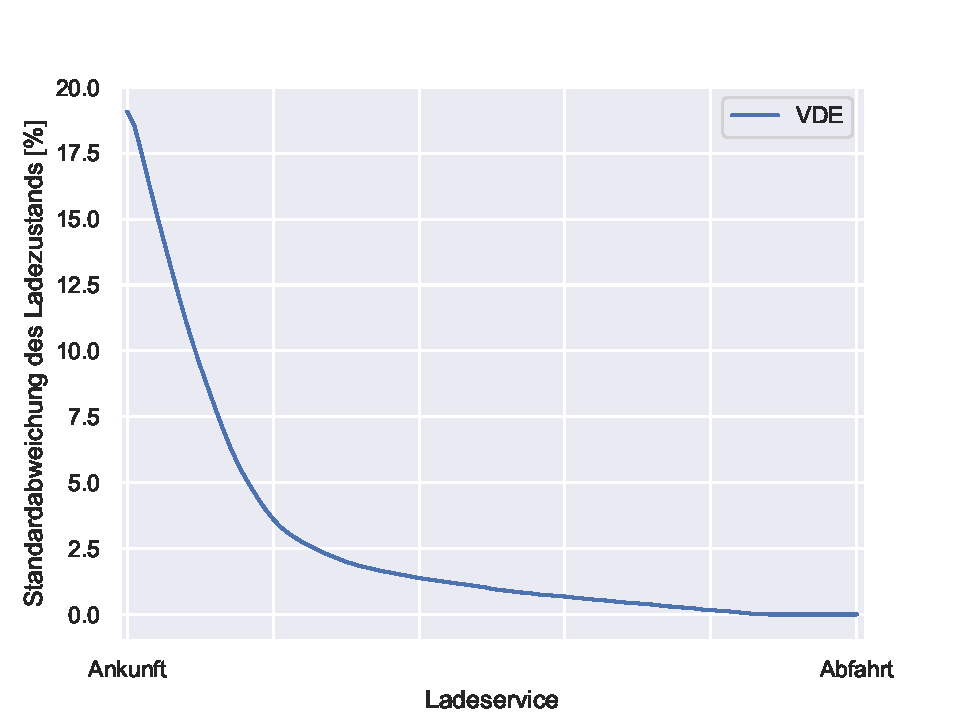
\includegraphics[width=\linewidth]{img/VDE_tau/tau_VDE_2_soc_std.pdf}
        \subcaption{Durschschnittliche Standardabweichung des Ladezustandes über den Verlauf eines Ladeservices}
        \label{ABB_VDEtauSocSTD}
	\end{subfigure}
\end{figure}

Da alle begonnen Ladeservices erfolgreich beendet wurden, ist die Qualität der Ladeservices maximal. Die Fairness beim Erreichen dieser Qualität ist in Abbildung \ref{Abb_VDEtauFairness} aufgezeichnet. \\
\begin{figure}[htb]
\centering
	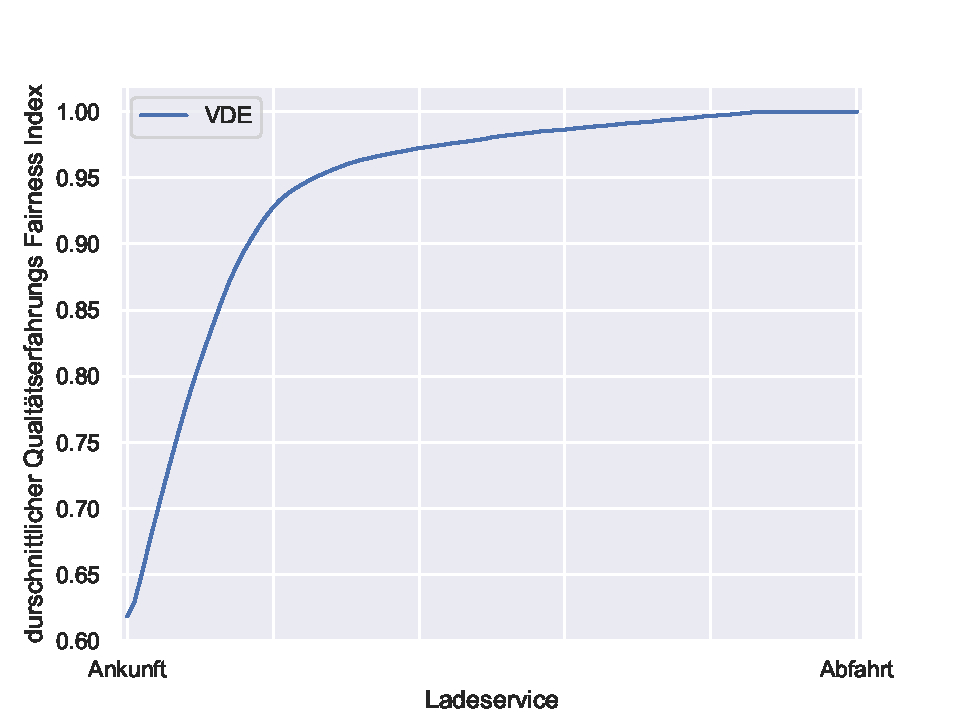
\includegraphics[scale=0.6]{img/VDE_tau/tau_VDE_2_qoe.pdf}
	\caption{Durchschnittlicher Qualitätserfahrung eines Elektrofahrzeuges über den Verlauf eines Ladeservices}
	\label{Abb_VDEtauFairness}
\end{figure}

Da die Fairness abhängig von der Standardabweichung des Ladezustandes ist, steigt die Fairness wie die Standardabweichung fällt. Da, je geringer die Standardabweichung ist, desto höher ist die Fairness. Die Fahrzeuge werden bereits in den Anfangszeiten der Ladeservices mit der nötigen Energie versorgt um einen Ladestand von 100 \% zu erreichen. Da diese Erhöhung des Ladestandes bei allen Teilnehmern so schnell von statten geht, sinkt auch die Standardabweichung schnell ab. Dieses Absinken zeigt die zunehmende Ähnlichkeit der Ladezustände und so auch die Fairness beim Laden.

\subsection{Slotted Aloha mit Teilnehmerzahl}
\label{chap_SApar}
Die Verwendung von SA participants wurde über den Zeitraum von einer Woche simuliert. Da bei der Verwendung dieses Controller Wartezeiten mithilfe von Zufallszahlen bestimmt werden, wurde die Simulation mit 10 verschiedenen Startwerten für die Bestimmung dieser Zufallszahlen durchgeführt. Dargestellt werden die Ergebnisse eines einzelnen Werktages, allerdings nicht die Ergebnisse eines einzelnen Durchlaufes, sondern der Mittelwert aller Durchläufe samt der zugehörigen Standartabweichung. Es wird der selbe Werktag wie bereits in Kapitel .. verwendet, um die Vergleichbarkeit der Ergebnisse zu gewährleisten. Dargestellt wird die Transformatorlast, die minimalen Werte der Spannung sowie die Anzahl der Teilnehmer, welche Leistung aus dem Netz beziehen. \\
\begin{figure}
	\begin{subfigure}{\linewidth}
		\includegraphics[scale=0.5]{img/SA_par/TrafoLast2.pdf}
		\caption{Transformatorlast über den Verlauf eines Tages}
		\label{Abb_SAparTrafoLast}
	\end{subfigure}
	\begin{subfigure}{\linewidth}
		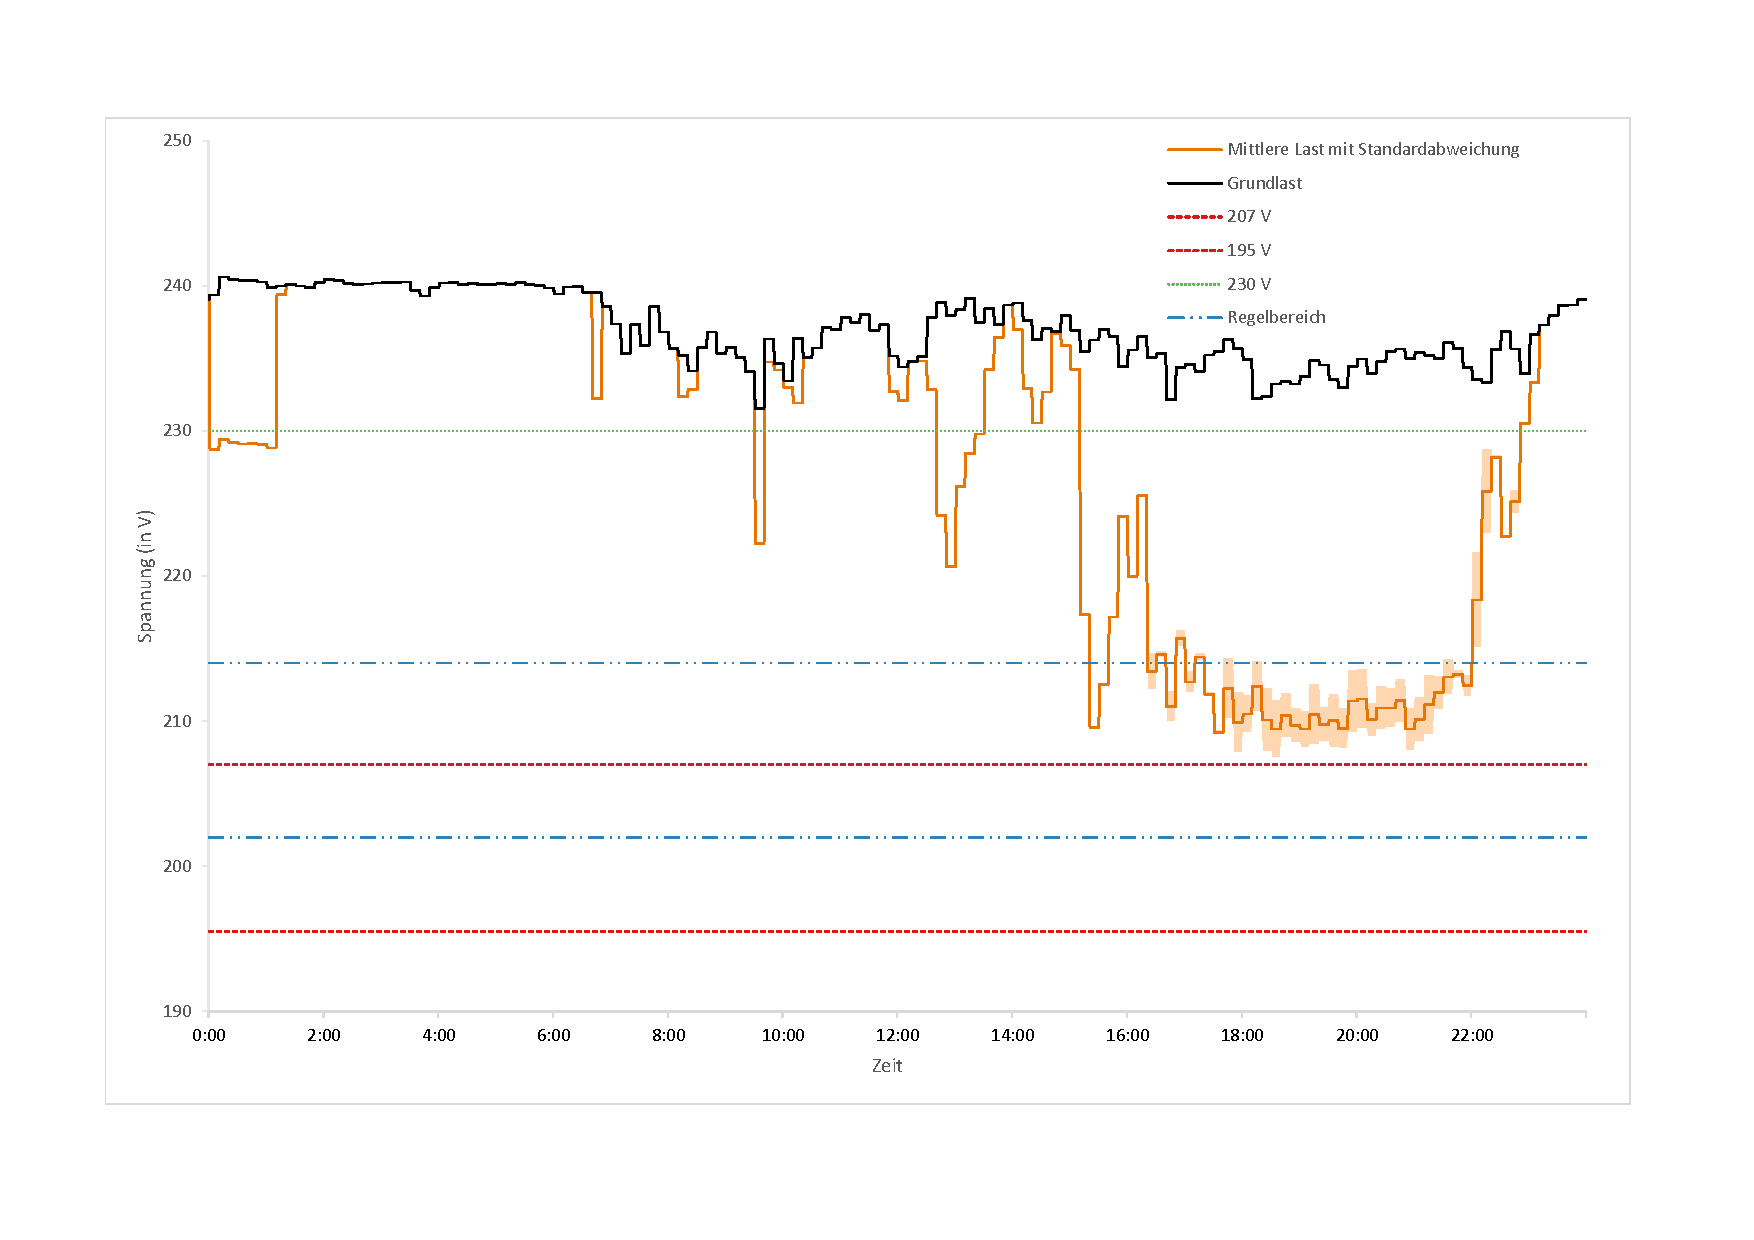
\includegraphics[scale=0.5]{img/SA_par/Voltage2.pdf}
		\caption{Spannungsverlauf mit 10 Minuten Mittelwerten bei Verwendung des VDE Spannungs-Controllers}
		\label{Abb_SAparSpannung}
	\end{subfigure}
\end{figure}

In der Abbildung \ref{Abb_SAparTrafoLast} ist die vom Transformator ans Niederspannungsnetz abgegebene Scheinleistung in kVA über den Verlauf eines Tages abgebildet. Der Regelbereich des Controllers ist im Falle der Transformatorlast nicht relevant, da der VDE Controller lediglich die Spannung berücksichtigt.\\
Abbildung \ref{Abb_SAparSpannung} zeigt den Verlauf der minimalen Spannung über das gesamte Niederspannungsnetz hinweg. Auch hier werden die Mittelwerte von 10 Minuten Intervallen zur Überprüfung der Norm DIN EN 50160 abgebildet.
\begin{figure}[htb]
\centering
	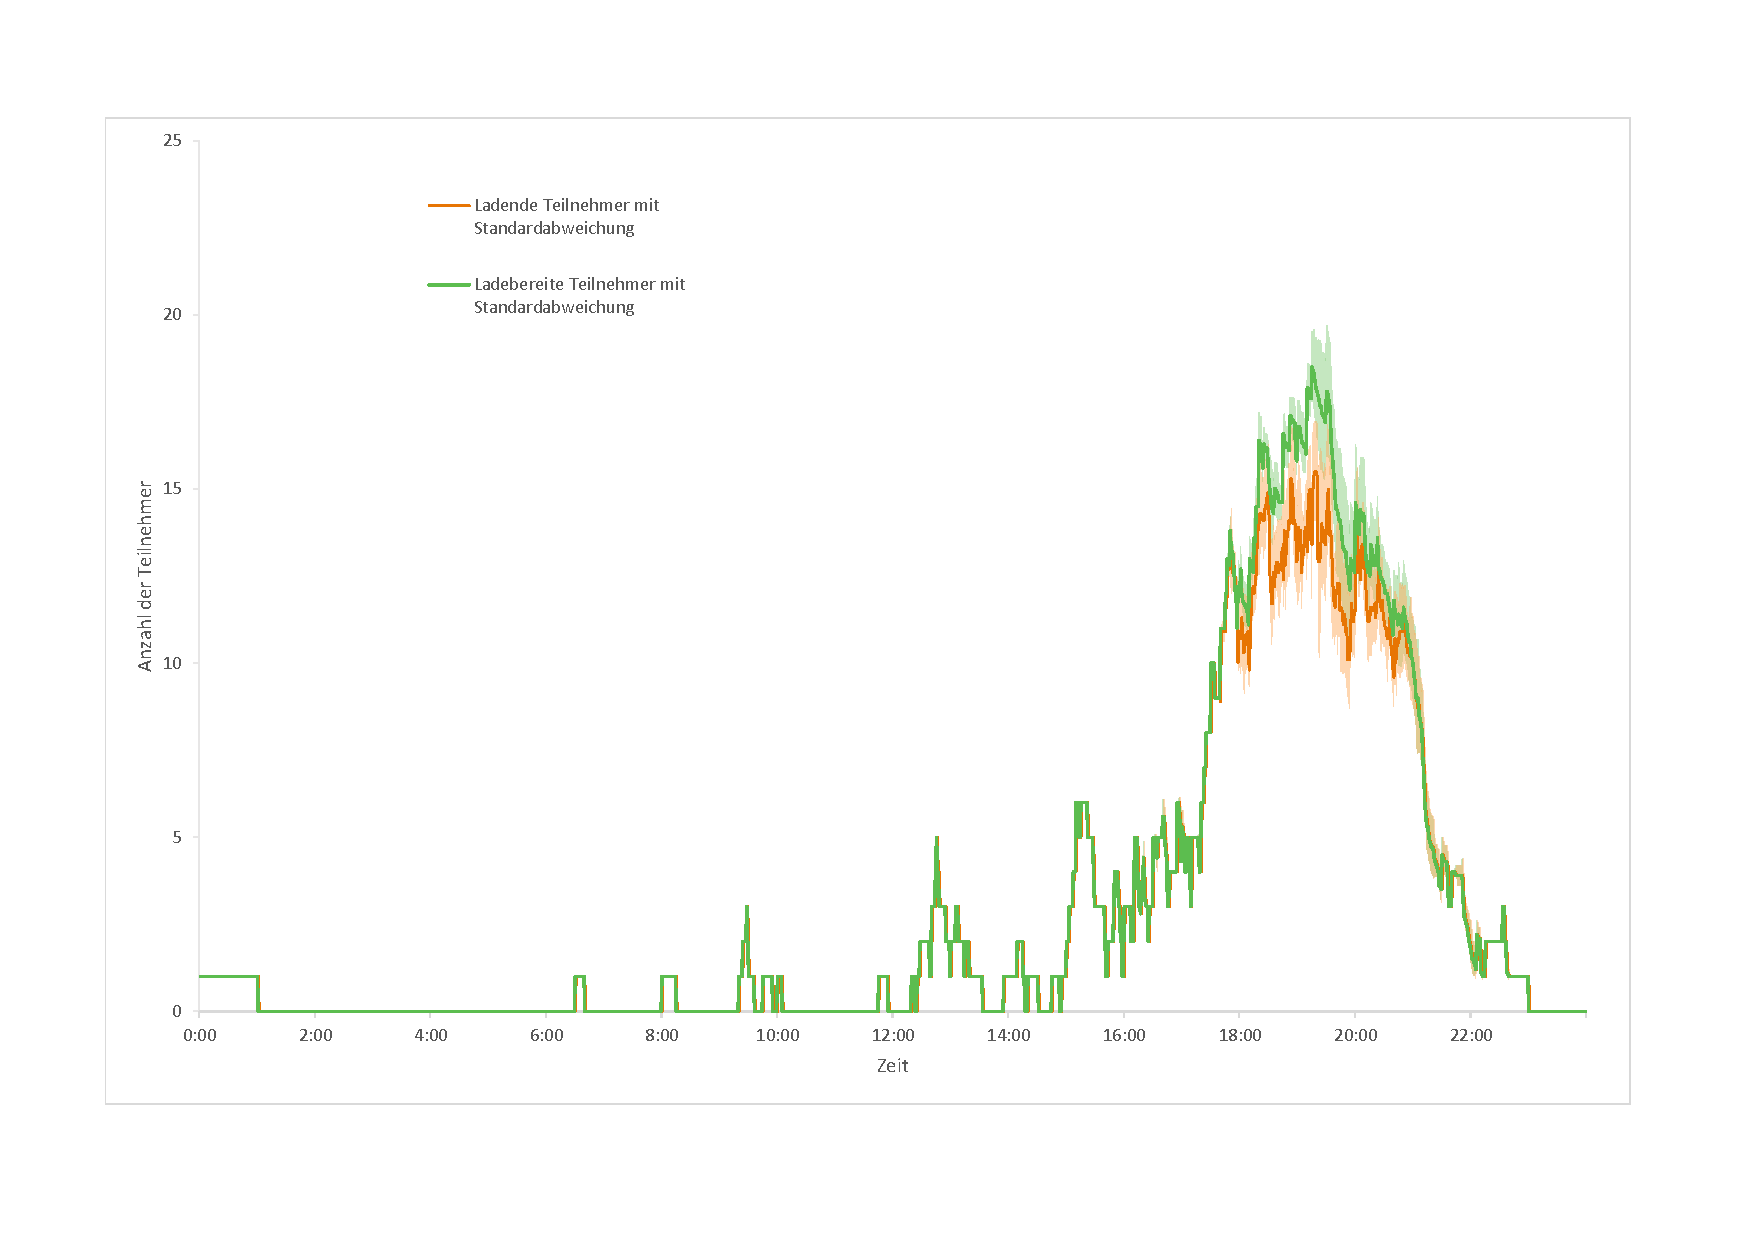
\includegraphics[scale=0.5]{img/SA_par/Teilnehmer_full.pdf}
	\caption{Teilnehmerzahlen über den Verlauf eines Tages}
	\label{Abb_SAparTeilnehmer}
\end{figure}
In der Abbildung \ref{Abb_SAparTeilnehmer} ist die Anzahl an Controllern abgebildet, welche Leistung für das Laden von Elektrofahrzeugen aus dem Netz beziehen. Leistungsbezieher, welche zwar Leistung beziehen, mit dieser aber kein Elektrofahrzeug laden, werden nicht dargestellt. \\
Bis etwa 16:00 steigt sowohl die Grundlast und somit auch die Transformatorlast als ganzes zwar mehrmals an, jedoch fällt die Spannung dadurch nie bis zum Regelbereich hin ab. Um etwa 16:00 fällt die Spannung erstmals in den Regelbereich ab, steigt dann allerdings wieder an. Dieser Spannungsfall lässt sich auf einen erhöhten Leistungsbedarf von der steigenden Anzahl an Teilnehmern zurückführen. Da die Anzahl an Teilnehmer nur kurz ansteigt, steigt auch die Spannung wieder an. Nach 16:00 fällt der Minimalwert der Spannung für etwa 6 Stunden bis in den Regelbereich ab. Im selben Zeitraum kommt es auch zu einem erhöhten Leistungsabgabe am Transformator, und auch die Anzahl der Teilnehmer steigt an auf bis zu 18 Teilnehmer. Innerhalb der Zeitspanne in der sich die Spannungswerte im Regelbereich des Spannungscontrollers befinden schwanken die minimalen Werte nur gering, sie bewegen sich von 215 V bis 209 V, also innerhalb einer Spanne von 6 Volt. Diese geringe Schwankung lässt den Schluss zu das diese Variante des Controllers in der Lage ist die Spannung im Niederspannungsnetz effektiv zu regeln und auf einem ausreichenden Niveau zu halten. \\
Im gesamten betrachteten Zeitraum von einer Woche kommt es zu keiner Unterschreitung der 195 Voltmarke sowie zu lediglich im Durchschnitt etwa 0,4 Unterschreitungen der 207 Volt Marke. Die Norm DIN EN 50160 wird folglich erfüllt, da die betrachteten Grenzwerte innerhalb der erlaubten Bereiche liegen.\\
Über den Simulationszeitraum hinweg wurden im Schnitt 668,7 Situationen (+- 6,7\%) festgestellt, in denen Spannungswerte gemessen wurden, welche eine Spannungskollision verursachen könnten. In 553,9 dieser 668,7 Situationen (+- 5,9\%) trat tatsächlich eine Spannungskollision auf und eine Wartezeit wurde berechnet. Der Simulationszeitraum umfasst 10080 Zeitschritte für 110 Teilnehmer, folglich wurden 1108800 Situationen betrachtet. Die 553,9 Situationen stellen also 0,04\% der insgesamt betrachteten Situationen dar. Die hier verwendete Methodik reagiert nur auf Spannungskollisionen, die Menge von Situationen in denen eine Transformatorkollision auftreten könnte wurde dennoch erfasst. In durchschnittlich 7514,5 (+- 2,0\%) der betrachteten Situationen wurde ein Verstoß gegen den Grenzwert der Transformatorlast festgestellt, was etwa 0,67\% aller Situation entspricht.\\
\begin{figure}
	\begin{subfigure}{0.49\linewidth}
		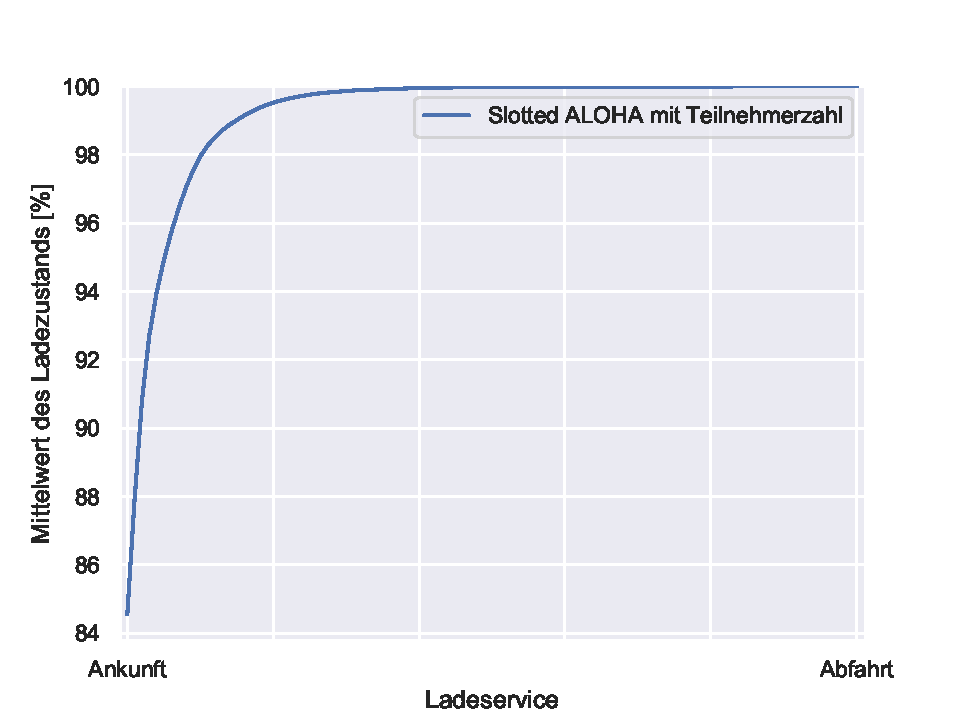
\includegraphics[width=\linewidth]{img/SA_par/SlottedAloha_participants_VDE_tau_10_soc_mean.pdf}
        \subcaption{Durchschnittlicher Ladezustand eines Elektrofahrzeuges über den Verlauf eines Ladeservices}
        \label{ABB_SAparSocMEAN}
	\end{subfigure}
	\begin{subfigure}{0.49\linewidth}
		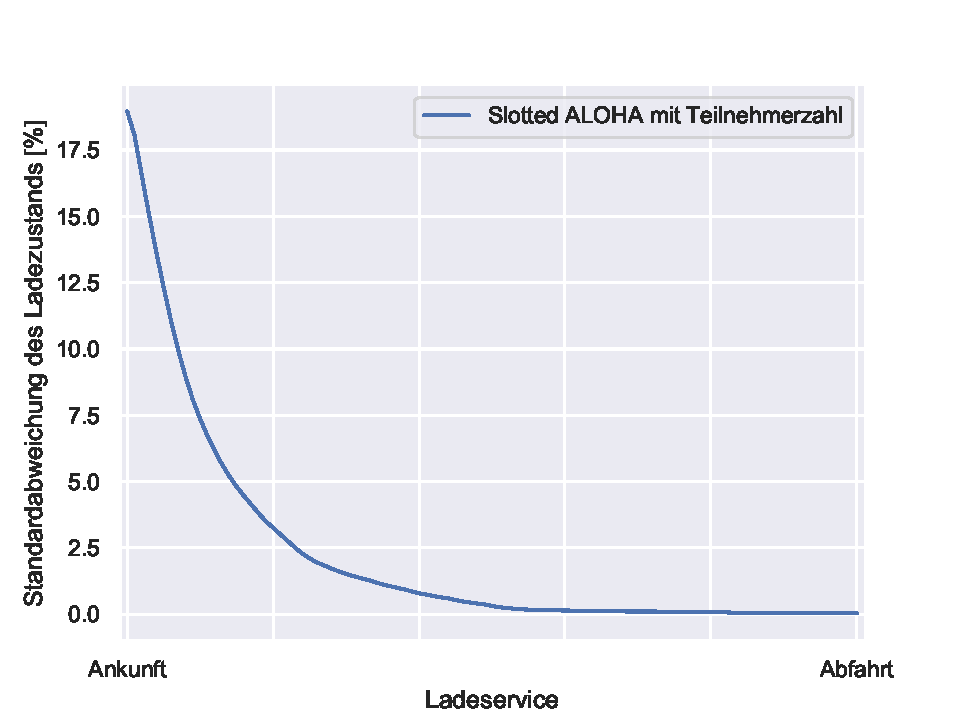
\includegraphics[width=\linewidth]{img/SA_par/SlottedAloha_participants_VDE_tau_10_soc_std.pdf}
        \subcaption{Durschschnittliche Standardabweichung des Ladezustandes über den Verlauf eines Ladeservices}
        \label{ABB_SAparSocSTD}
	\end{subfigure}
\end{figure}
Alle 557 gestarteten Ladeservices wurden erfolgreich abgeschlossen, somit ist die Qualitätserfahrung aller Ladevorgänge maximal. Abbildung \ref{ABB_SAparSocMEAN} zeigt den durchschnittlichen Ladezustand über den Verlauf eines Ladeservices hinweg, Abbildung \ref{ABB_SAparSocSTD} zeigt die zugehörige Standardabweichung. Ein schneller Anstieg des mittleren Ladezustands zeigt das Fahrzeuge bereits zu Beginn des jeweiligen Ladeservices mit dem Laden beginnen. Nach etwa 20\% der Zeit hat sich der mittlere Ladestand von etwa 85\% auf etwa 99\% erhöht und hat damit den Zielwert von 100\% fast erreicht. Die zu diesem Zeitpunkt mit etwas über 2,5\% ebenfalls bereits gesunkene Standardabweichung weist auf eine Angleichung der jeweiligen Werte hin.
\begin{figure}[htb]
\centering
	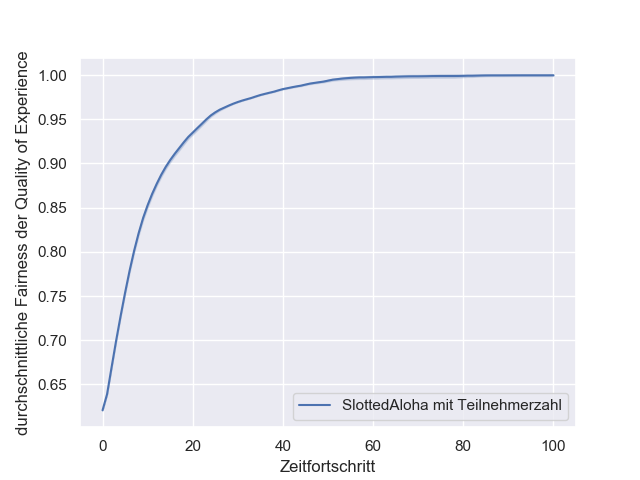
\includegraphics[scale=0.6]{img/SA_par/SlottedAloha_participants_VDE_tau_10_qoe.png}
	\caption{Durchschnittlicher Qualitätserfahrung eines Elektrofahrzeuges über den Verlauf eines Ladeservices}
	\label{Abb_SAparFairness}
\end{figure}
Abbildung \ref{Abb_SAparFairness} zeigt die Fairness der jeweiligen Qualitätserfahrung über den Zeitverlauf der Ladeservices. Die Qualität des Ladeservices hängt von der Standardabweichung des Ladezustandes ab. Der schnelle Anstieg des Graphen, in den ersten 20\% der Zeit er höht sich der Wert von etwa 0,65 um etwa 0,3 auf ca. 0,95 und liegt so nach nur 20\% schon nahe am Idealwert von 1. Der Idealwert wird nach etwa 50\% der Zeit erreicht, ab diesem Zeitpunkt herrscht höchstmögliche Fairness zwischen den Teilnehmern.

\subsection{Slotted Aloha mit Teilnehmerzahl und Fahrzeugparametern}
\label{chap_SAwt}
Die Verwendung des Spannungskontrolles, welcher mit Slotted Aloha erweitert wurde und die Teilnehmeranzahl und die Fahrzeugparameter miteinbezieht. Diese Variante des Controller bestimmt mögliche Wartezeiten unter anderem mit der Hilfe von Zufallszahlen. Die Simulation wurde mit 10 verschieden Startwerten für die Bestimmung dieser Zufallszahlen durchgeführt. Dargestellt werden die Ergebnisse eines einzelnen Werktages, allerdings nicht die Ergebnisse eines einzelnen Durchlaufes, sondern der Mittelwert aller Durchläufe samt der zugehörigen Standartabweichung. Es wird der selbe Werktag wie bereits in Kapitel .. verwendet, um die Vergleichbarkeit der Ergebnisse zu gewährleisten. Dargestellt wird die Transformatorlast, die minimalen Werte der Spannung sowie die Anzahl der Teilnehmer, welche Leistung aus dem Netz beziehen. 
\begin{figure}
	\begin{subfigure}{\linewidth}
		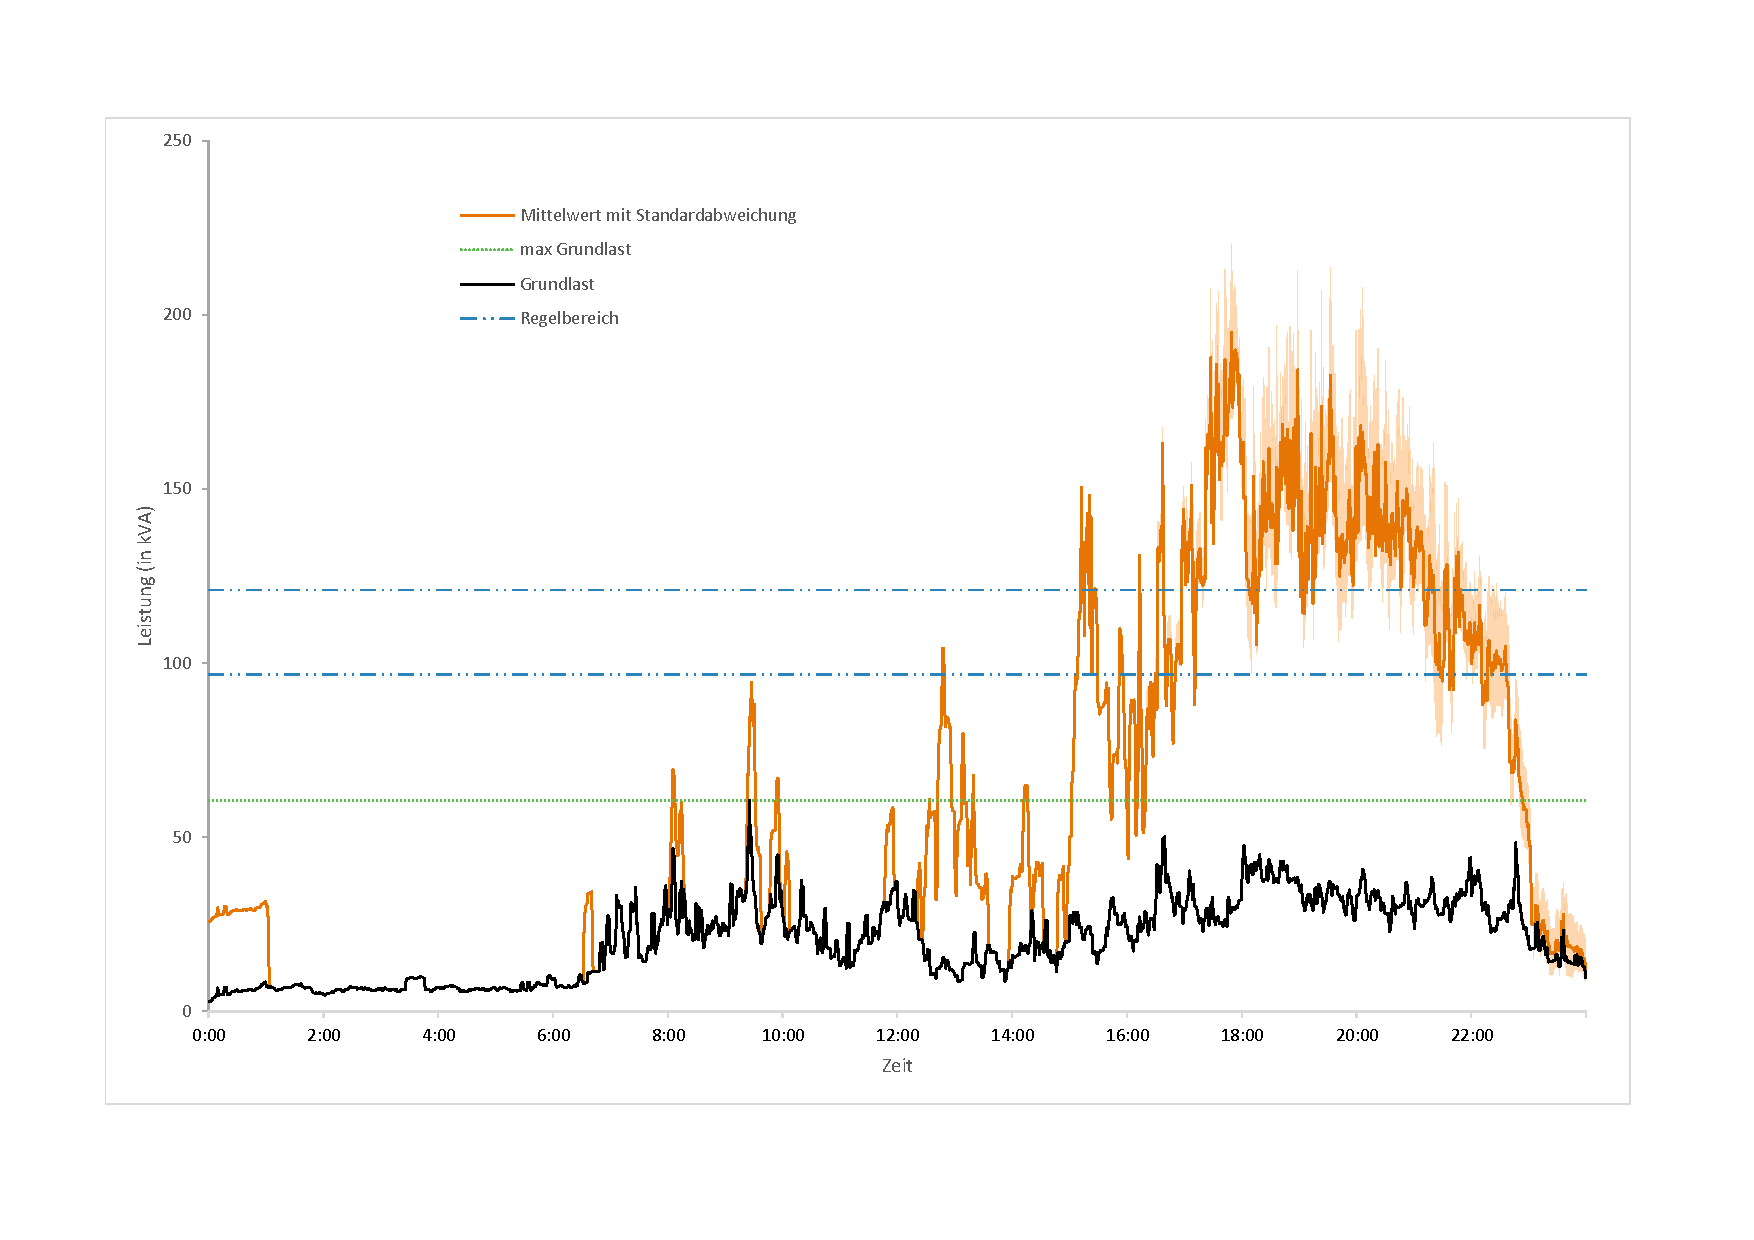
\includegraphics[scale=0.5]{img/SA_wT/TrafoLast4.pdf}
		\caption{Transformatorlast über den Verlauf eines Tages}
		\label{Abb_SAwtTrafoLast}
	\end{subfigure}
	\begin{subfigure}{\linewidth}
		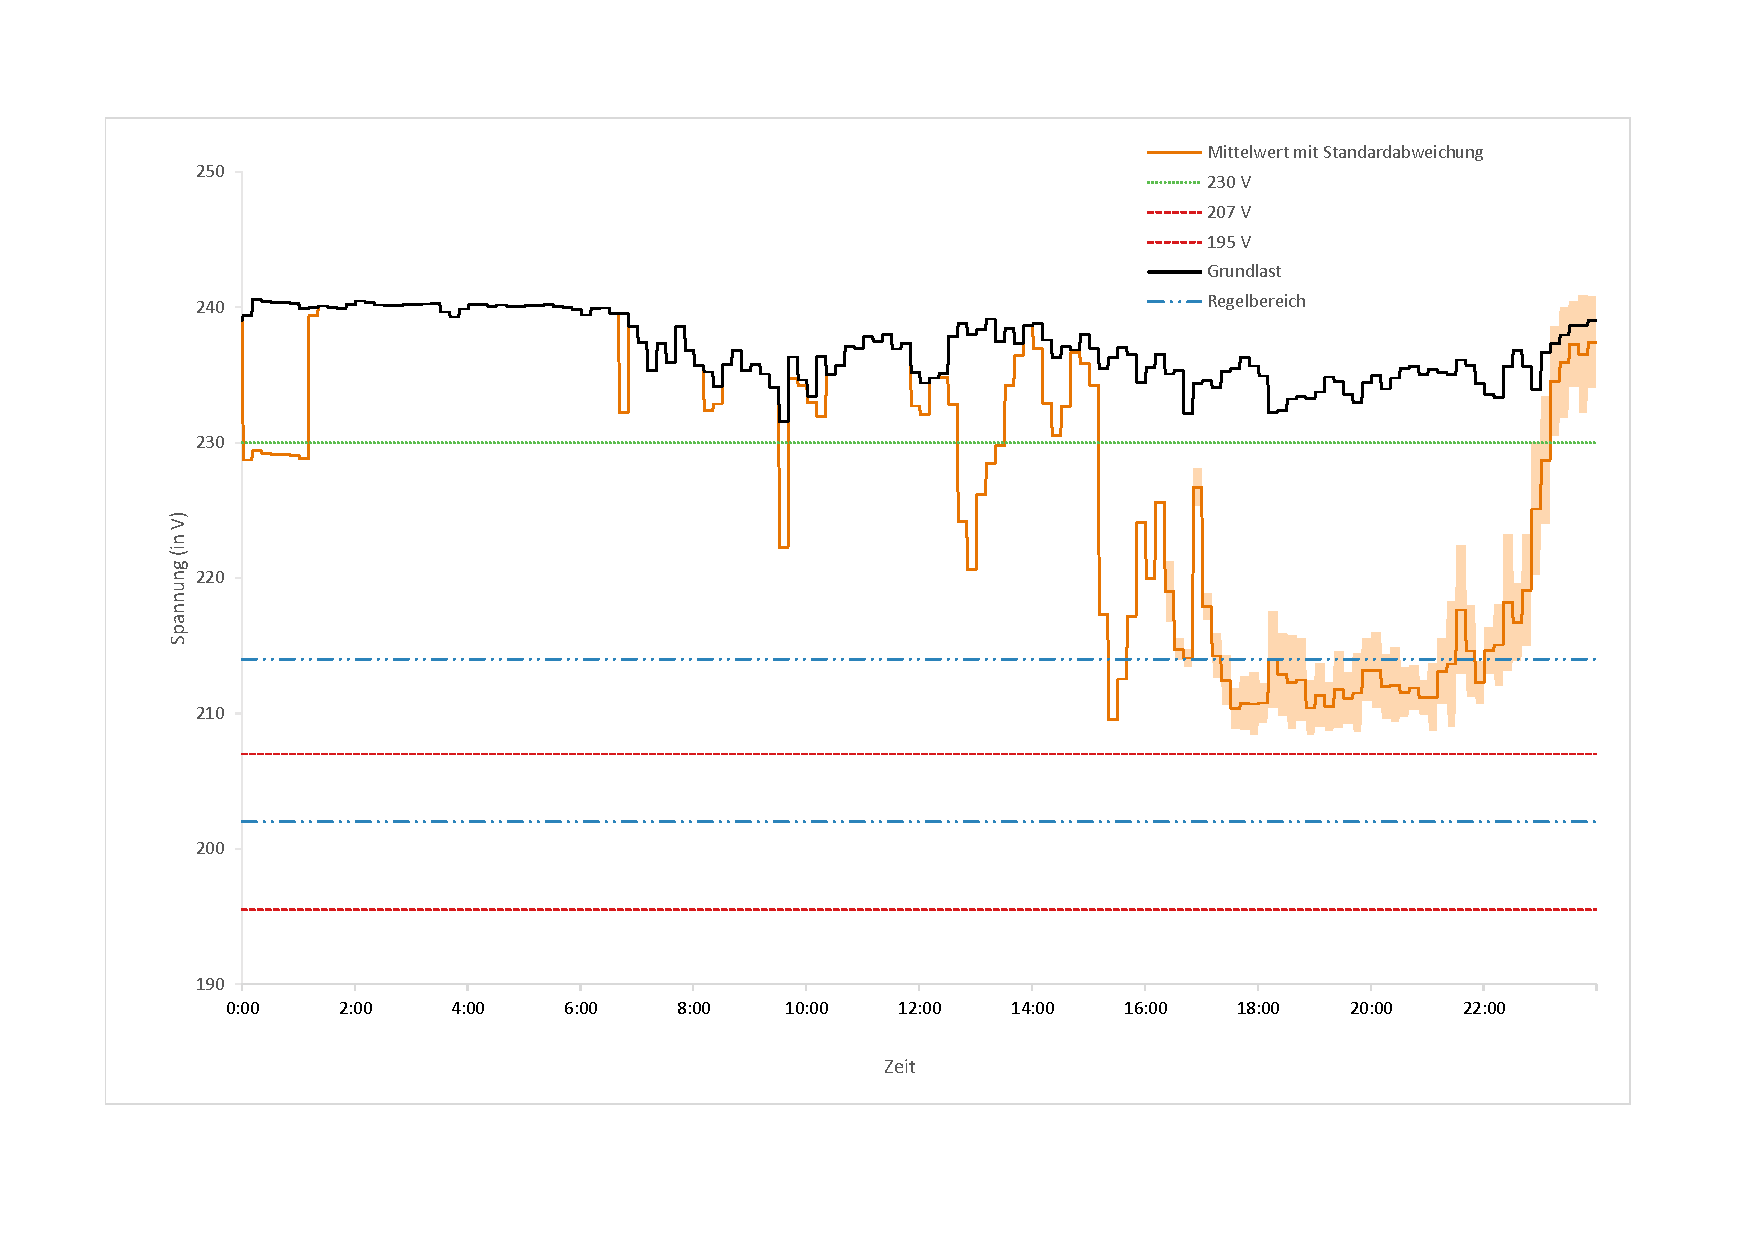
\includegraphics[scale=0.5]{img/SA_wT/Voltage.pdf}
		\caption{Spannungsverlauf in 10 Minuten Intervallen über den Verlauf eines Tages}
		\label{Abb_SAwtSpannung}
	\end{subfigure}
\end{figure}

In der Abbildung \ref{Abb_SAwtTrafoLast} ist die vom Transformator ans Niederspannungsnetz abgegeben Scheinleistung in kVA über den Verlauf eines Tages abgebildet. Der Regelbereich des Controllers ist im Falle der Transformatorlast nicht relevant, der VDE Controller lediglich die Spannung berücksichtigt.\\
Abbildung \ref{Abb_SAwtSpannung} zeigt den Verlauf der minimalen Spannung über das gesamte Niederspannungsnetz hinweg. Auch hier werden die Mittelwerte von 10 Minuten Intervallen zur Überprüfung der Norm DIN EN 50160 abgebildet.
\begin{figure}[htb]
\centering
	\includegraphics[scale=0.5]{img/SA_wT/Teilnehmer2.pdf}
	\caption{Teilnehmerzahl über den Verlauf eines Tages}
	\label{Abb_SAwtTeilnehmer}
\end{figure}

In der Abbildung \ref{Abb_SAwtTeilnehmer} ist die Anzahl an Controllern abgebildet, welche Leistung für das Laden von Elektrofahrzeugen aus dem Netz beziehen. Leistungsbezieher, welche zwar Leistung beziehen, mit dieser aber kein Elektrofahrzeug laden, werden nicht dargestellt. \\
Die Aktivitäten bis etwa 16:00 führen zwar immer wieder zu einem Absinken der Spannung, jedoch erreichen die Werte dabei den Regelbereich des Controllers nicht. Um etwa 16:00 fällt der Spannungswert das erste Mal bis in den Regelbereich hinein ab, erholt sich dann aber wieder. Dieser kurze Abfall lässt sich auf eine kurzfristig ansteigende Anzahl an Teilnehmer und so auch steigende Transformatorlast zurückführen. Von etwa 17:00 bis 21:00 befinden sich die Mittelwerte der Minimalspannung durchgängig im Regelungsbereich des Controllers. Die Werte bewegen sich im Bereich von 217 V bis 210 V, schwanken in diesem Zeitraum also nur um etwa 7 V. Die geringe Schwankung der Werte sowie fehlende Unterschreitungen des Regelbereiches lässt den Schluss zu das diese variante des Controllers dazu in der Lage ist die Spannung effektiv zu regeln und sie auf einem ausreichenden Niveau zu halten.
Im gesamten betrachteten Zeitraum von einer Woche kommt es zu keiner Unterschreitung der 195 Voltmarke sowie zu lediglich im Durchschnitt etwa 0,4 Unterschreitungen der 207 Volt Marke. Die Norm DIN EN 50160 wird folglich erfüllt, da die betrachteten Grenzwerte innerhalb der erlaubten Bereiche liegen.\\
Über den Simulationszeitraum hinweg wurden im Schnitt 392,6 Situationen (+- 12,2\%) festgestellt, in denen Spannungswerte gemessen wurden, welche eine Spannungskollision verursachen könnten. In 246,9 dieser 392,6 Situationen (+- 9,2\%) trat tatsächlich eine Spannungskollision auf und eine Wartezeit wurde berechnet. Der Simulationszeitraum umfasst 10080 Zeitschritte für 110 Teilnehmer, folglich wurden 1108800 Situationen betrachtet. Die 246,9 Situationen stellen also 0,02\% der insgesamt betrachteten Situationen dar. Die hier verwendete Methodik reagiert nur auf Spannungskollisionen, die Menge von Situationen in denen eine Transformatorkollision auftreten könnte wurde dennoch erfasst. In durchschnittlich 9271,5 (+- 3,3\%) der betrachteten Situationen wurde ein Verstoß gegen den Grenzwert der Transformatorlast festgestellt, was etwa 0,83\% aller Situationen entspricht.\\
\begin{figure}
	\begin{subfigure}{0.49\linewidth}
		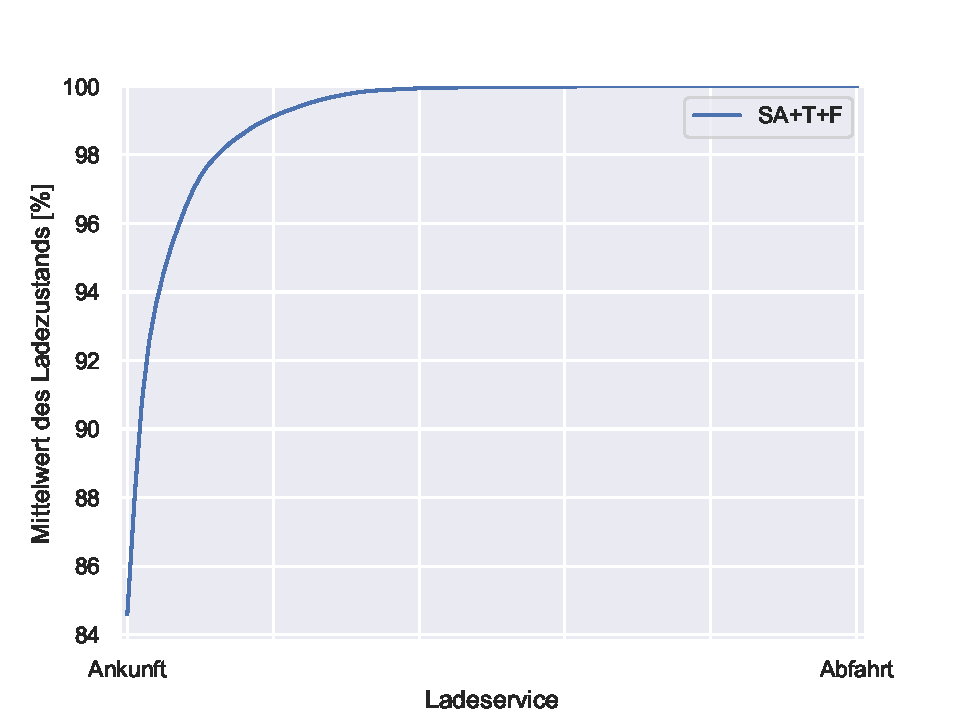
\includegraphics[width=\linewidth]{img/SA_wT/SlottedAloha_waitingTime_VDE_tau_6_soc_mean.pdf}
        \subcaption{Durchschnittlicher Ladezustand eines Elektrofahrzeuges über den Verlauf eines Ladeservices}
        \label{ABB_SAwtSocMEAN}
	\end{subfigure}
	\begin{subfigure}{0.49\linewidth}
		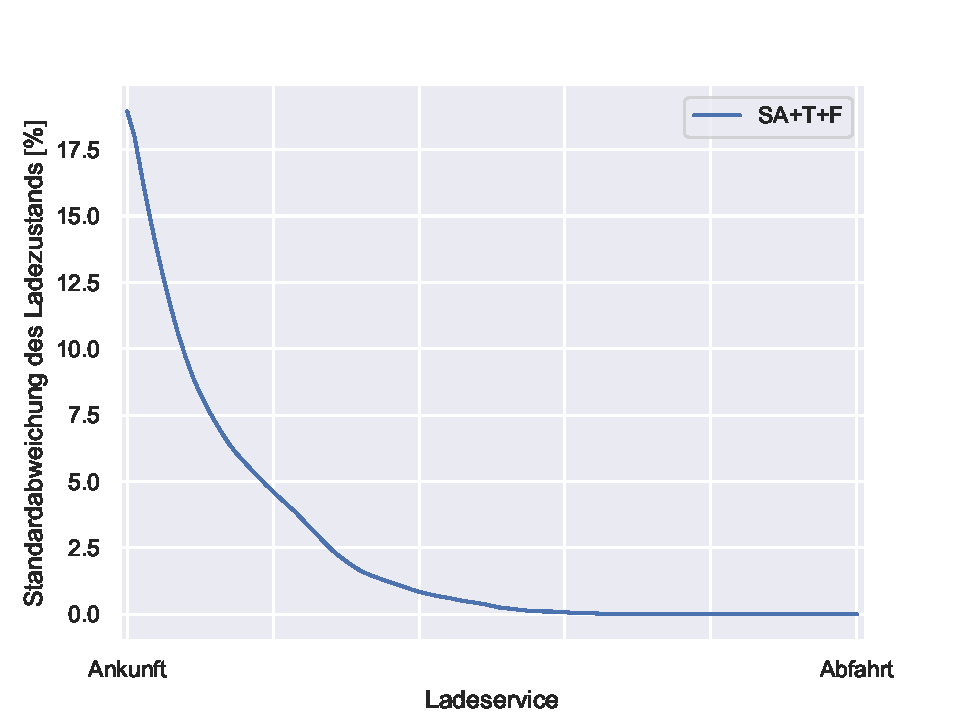
\includegraphics[width=\linewidth]{img/SA_wT/SlottedAloha_waitingTime_VDE_tau_6_soc_std.pdf}
        \subcaption{Durschschnittliche Standardabweichung des Ladezustandes über den Verlauf eines Ladeservices}
        \label{ABB_SAwtSocSTD}
	\end{subfigure}
	\caption{ganz unten}
\end{figure}

Alle 557 gestarteten Ladeservices wurden erfolgreich abgeschlossen, somit ist die Qualitätserfahrung aller Ladevorgänge maximal. Abbildung \ref{ABB_SAwtSocMEAN} zeigt den durchschnittlichen Ladezustand über den Verlauf eines Ladeservices hinweg, Abbildung \ref{ABB_SAwtSocSTD} zeigt die zugehörige Standardabweichung. Ein schneller Anstieg des mittleren Ladezustands zeigt das Fahrzeuge bereits zu Beginn des jeweiligen Ladeservices mit dem Laden beginnen. Nach etwa 20\% der Zeit hat sich der mittlere Ladestand von etwa 85\% auf etwa 99\% erhöht und hat damit den Zielwert von 100\% fast erreicht. Die zu diesem Zeitpunkt mit etwas unter 5\% ebenfalls bereits gesunkene Standardabweichung weist auf eine Angleichung der jeweiligen Werte hin.\\
\begin{figure}[htb]
\centering
	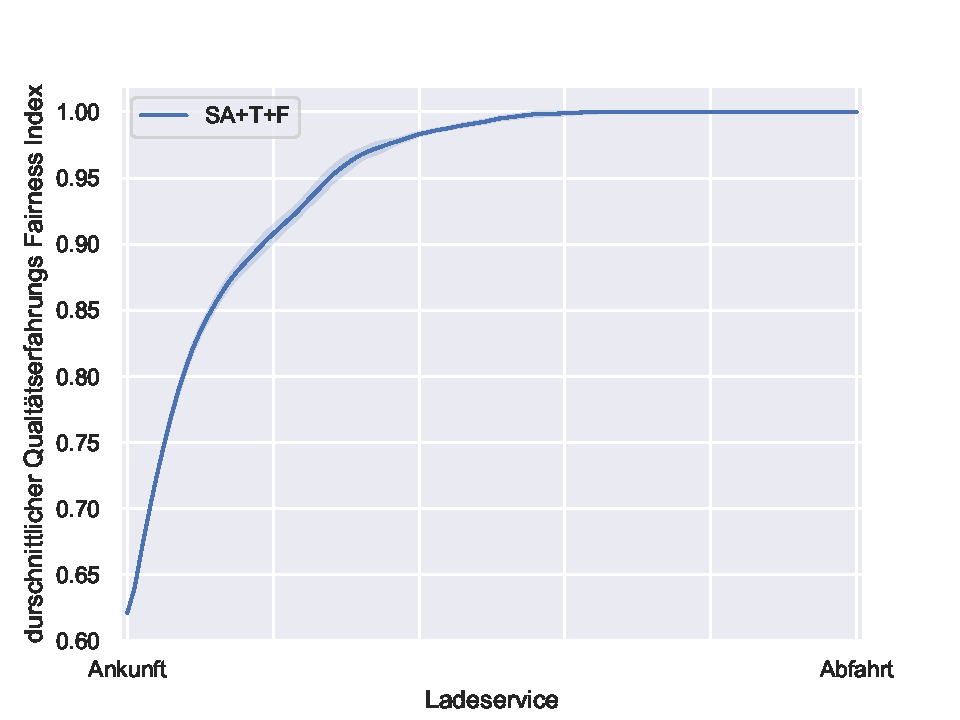
\includegraphics[scale=0.6]{img/SA_wT/SlottedAloha_waitingTime_VDE_tau_6_qoe.pdf}
	\caption{Durchschnittlicher Qualitätserfahrung eines Elektrofahrzeuges über den Verlauf eines Ladeservices}
	\label{Abb_SAwTFairness}
\end{figure}

Abbildung \ref{Abb_SAwTFairness} zeigt die Fairness der jeweiligen Qualitätserfahrung über den Zeitverlauf der Ladeservices. Die Qualität des Ladeservices hängt ab von der Standardabweichung des Ladezustandes ab. Der schnelle Anstieg des Graphen, in den ersten 20\% der Zeit er höht sich der Wert von etwa 0,65 um etwa 0,25 auf ca. 0,9 und liegt so nach nur 20\% schon nahe am Idealwert von 1. Der Idealwert wird nach etwa 50\% der Zeit erreicht, ab diesem Zeitpunkt herrscht höchstmögliche Fairness zwischen den Teilnehmern.

\subsection{VDE-Controller mit Transformatorkontroller}
\label{chap_VDE_t}
Eine weitere betrachtete Methodik ist der VDE-Controller, welcher an sich nur ein Spannungscontroller ist, hier aber um den in dieser Arbeit entwickelten Transformatorkontroller erweitert wurde. Für diese Kombination musste der eigentlich mit dem Transformatorkontroller veränderte lag-Filter nochmals geändert werden. Diese erneute Änderung war nötig, da bei Verwendung des angedachten Lag-Filters  die Werte der Spannung an einem Punkt im simulierten Zeitraum so stark gefallen sind, das PyPower nicht mehr in der Lage war diese Werte zu berechnen und die Simulation vorzeigt beendet werden musste. Bei der Verwendung des Lag-Filters, wie er ursprünglich in Kapitel .. eingeführt wurde, trat dieses Problem nicht auf und die Simulation konnte erfolgreich beendet werden. Die Simulation umfasst auch hier den Zeitraum von einer Woche und wird ebenfalls gemäß der Transformatorlast, der Spannung, der Teilnehmerzahl, der Kollisionsanzahl, der Quality of Experince und der Fairness untersucht. Bei der Transformatorlast, der Spannung, der Teilnehmerzahl wird erneut nur ein Werktag aus der durchlaufenen Woche dargestellt, um eine bessere Übersichtlichkeit der Graphen zu erreichen. \\
\begin{figure}
	\begin{subfigure}{\linewidth}
		\includegraphics[scale=0.5]{img/VDE_tau_trafo/TrafoLast2.pdf}
		\caption{Transformatorlast über den Verlauf eines Tages}
		\label{Abb_VDETrafo_TrafoLast}
	\end{subfigure}
	\begin{subfigure}{\linewidth}
		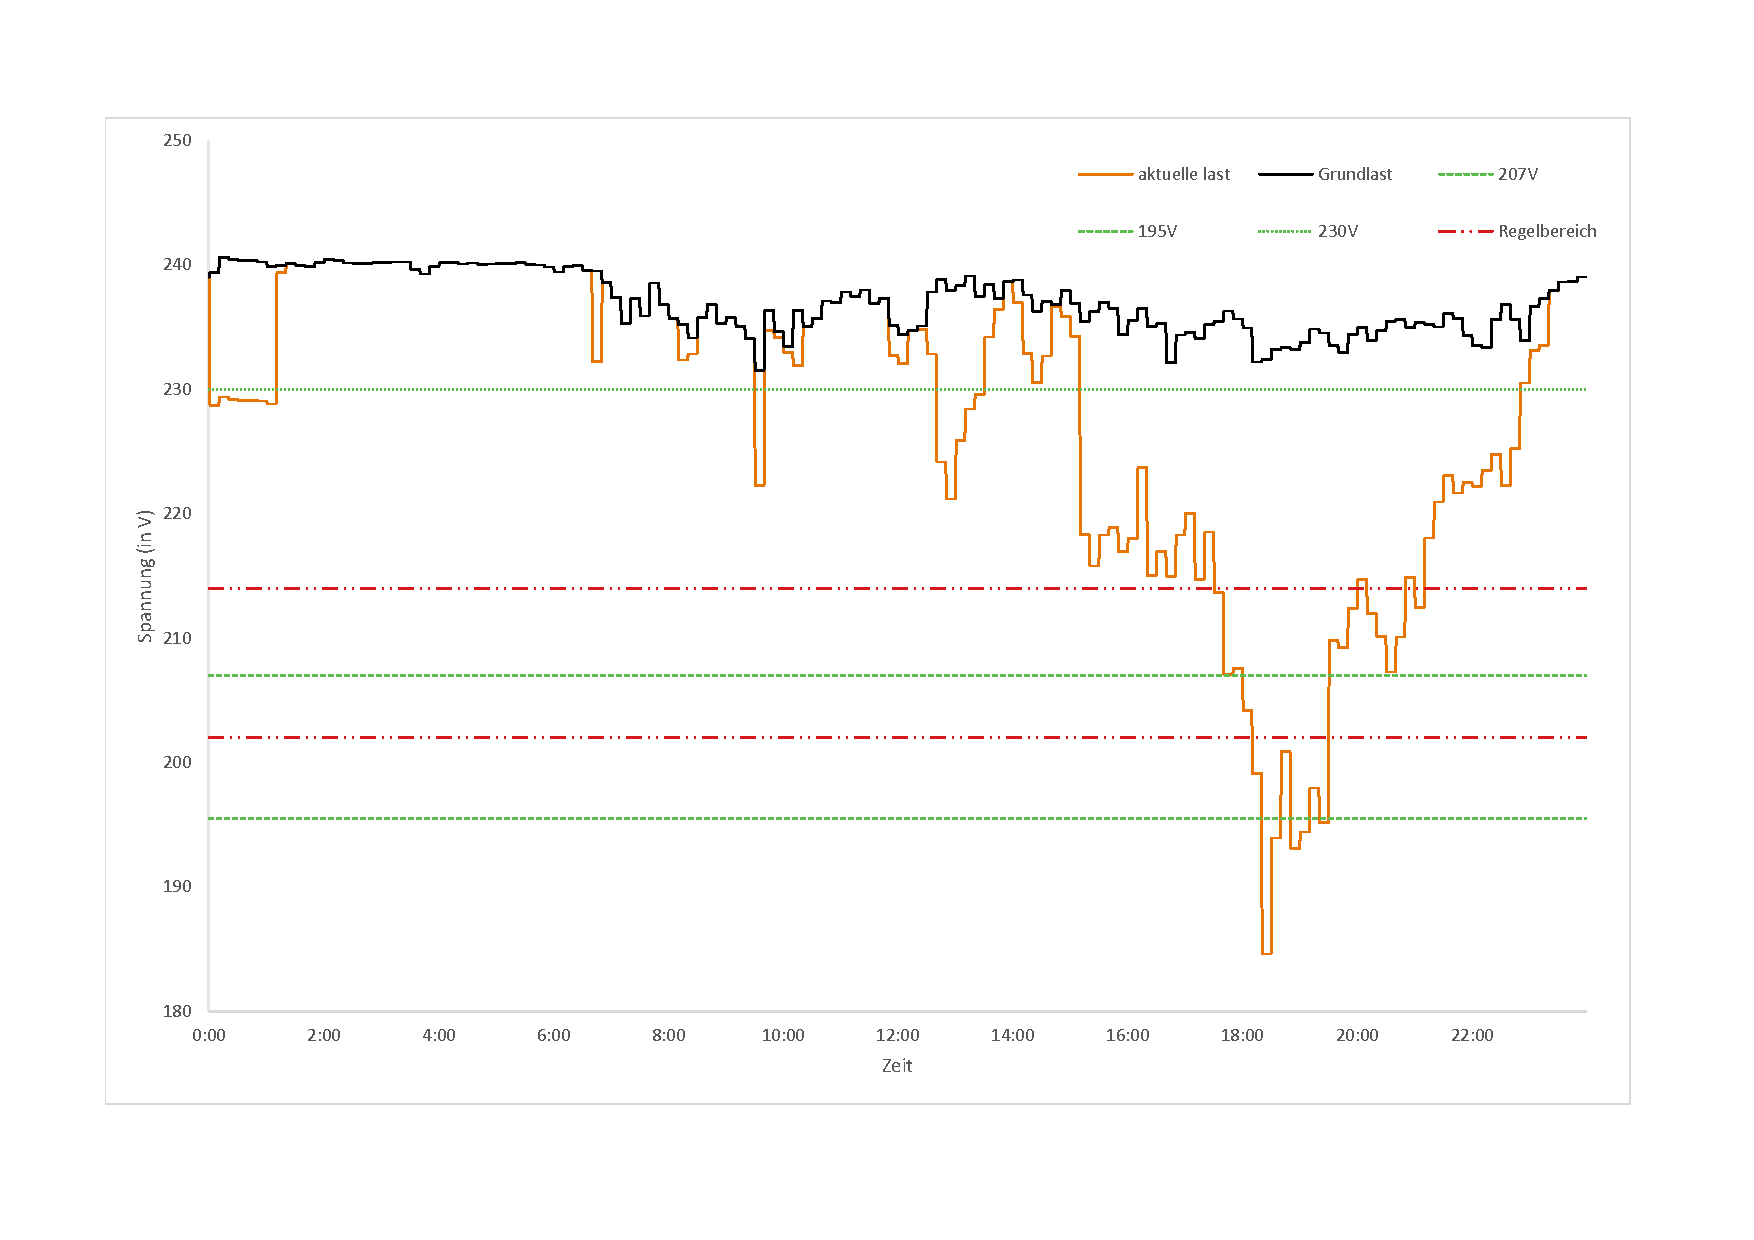
\includegraphics[scale=0.5]{img/VDE_tau_trafo/Spannung2.pdf}
		\caption{10 Minuten Mittelwerte der Spannung über den Verlauf eines Tages}
		\label{Abb_VDETrafo_Spannung}
	\end{subfigure}
\end{figure}

In Abbildung \ref{Abb_VDETrafo_TrafoLast} ist die Menge der Scheinleistung dargestellt, welche vom Transformator ans Niederspannungsnetz abgegeben wird. Bei dieser Methodik werden keine Wartezeiten bestimmt, somit waren bei dieser Methodik keine mehrfachen Durchläufe nötig, somit gibt es auch keine Standardabweichung, da es auch keinen Mittelwert gibt. Der Verlauf des Graphen zeigt, dass der verwendet Transformatorkontroller nur bedingt bzw. nicht den angedachten Zweck erfüllt. Auch nach der Veränderung des Lag-Filters ist bei dieser Methodik nicht gelungen, die Transformatorlast zu kontrollieren und so zu limitieren. Der Graphen hat große Ähnlichkeit mit dem Ergebnis des VDE-Kontrollers ohne die Erweiterung des Transformatorkontrollers, auch das weist daraufhin das der Transformatorkontroller seinen Zweck nicht erfüllen kann. \\
In Abbildung \ref{Abb_VDETrafo_Spannung} sind die Mittelwerte der minimalen 10 Minuten Mittelwerte der Spannung angetragen. Auch in dieser Abbildung ist der Regelbereich des Spannungscontrollers abgebildet. Ebenso wie bereits beim Transformatorkontroller muss hier allerdings festgestellt werden, das der Spannungskontroller nicht ordentlich arbeitet, da die Werte nicht im oder über dem Regelbereich gehalten werden können. Das schnelle Absinken der Spannungswerte zeigt auch eine Überforderung des verwendeten Kontrollers an, da innerhalb nur weniger Messwerte der komplette Regelbereich durchlaufen wurde.\\
\begin{figure}[htb]
\centering
	\includegraphics[scale=0.5]{img/VDE_tau_trafo/Teilnehmer2.pdf}
	\caption{Anzahl der ladebereiten und tatsächlich ladenen Teilnehmer am Niederspannungsnetz über den Verlauf eines Tages}
	\label{Abb_VDETrafo_Teilnehmer}
\end{figure}

Abbildung \ref{Abb_VDETrafo_Teilnehmer} zeigt die Anzahl der ladebereiten und tatsächlich ladenden Teilnehmer an. Der geringe Abstand der beiden Kurven liegt an dem Fehlen von Wartezeiten bei dieser Methodik, welche Teilnehmer vom laden abhalten würden. Die Abweichungen der Graphen, welche trotzdem vorkommen, sind der Funktionsweise der Kontroller geschuldet, welche bei Unter- bzw. Überschreitung des Regelbereichs den Leistungsbezug unterbinden, dies allerdings nur für das jeweils aktuelle Zeitintervall. 
In dem Zeitraum von 0:00 bis etwa 15:00 befinden sich die Werte der Transformatorauslastung nur kurz im Regelbereich, die Spannungswerte fallen in dieser Zeitspanne gar nicht in den Regelbereich ab. Ab 15:00 nähern sich die Werte der Transformatorauslastung und der Spannung dem Regelbereich zunächst nur an, was sich auf die steigende Zahl der Teilnehmer zurückführen lässt. Ab ca. 16:00 nimmt die Zahl der Teilnehmer zuerst schnell zu, was in einem starken Abfall der Spannung und einer aufgrund starker Schwankungen nur teils hohen Transformatorlast endet. Mit einem Fallen der Teilnehmerzahl ab etwa 19:00, erholen sich auch die Spannungswerte und die Transformatorauslastung wieder. Zu diesem Zeitpunkt ist allerdings sowohl gegen den Transformatorkontroller und gegen den Spannungskontroller massiv verstoßen worden.
Aufgrund der massiven Verstöße gegen den Spannungskontroller schon an dem einem betrachtetem Tag, konnte die Einhaltung der Norm DIN EN 50160 nicht mehr erreicht werden. Der Schwellenwert von -10 \% p.u. wird bei mindesten einem Teilnehmer bis zu 17 Mal unterschritten, was noch innerhalb des Möglichen liegt, allerdings wird auch der Grenzwert von -15 \% p.u. unterschritten. Aufgrund von Unterschreitungen des Schwellenwerts bei -15 \% p.u. ist die Norm nicht erfüllt.
Bei dieser Methodik wird zwar sowohl der Spannungskontroller, als auch der Transformatorkontroller verwendet, jedoch werden keinerlei Wartezeiten bestimmt, mit denen auf möglicherweise aufgetreten Kollisionen reagiert werden könnte. Es wurden über den simulierten Zeitraum von einer Woche 1882 Situationen festgestellt, in denen eine zu niedrige Spannung gemessen wurde, und 5946 Situationen in denen eine zu hohe Auslastung des Transformators festgestellt wurde. Insgesamt kam es zu 5964 Situationen, in denen eine Wartezeit hätte bestimmt werden können, da dies bei dieser Methodik allerdings nicht vorgesehen ist, wurden keine Wartezeiten berechnet.
Alle im betrachteten Simulationszeitraum gestarteten Ladeservice wurden erfolgreich abgeschlossen, nicht ein Fahrzeug musste die Ladestation mit einem Ladestand von weniger als 100 \% verlassen. Da alle Ladeservice erfolgreich abgeschlossen wurden, ist die Qualität der Ladeservice maximal.
\begin{figure}
	\begin{subfigure}{0.49\linewidth}
		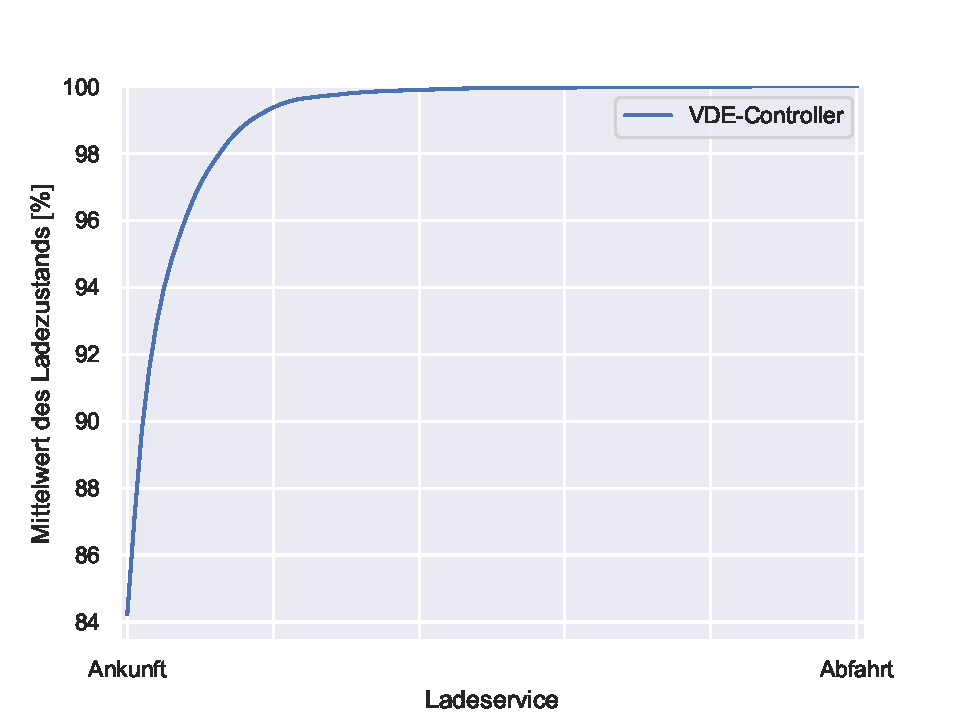
\includegraphics[width=\linewidth]{img/VDE_tau_trafo/tau_VDE_trafo_2_soc_mean.pdf}
        \subcaption{Durchschnittlicher Ladezustand aller Elektrofahrzeuges über den Verlauf eines Ladeservices}
        \label{ABB_VDETrafo_SocMEAN}
	\end{subfigure}
	\begin{subfigure}{0.49\linewidth}
		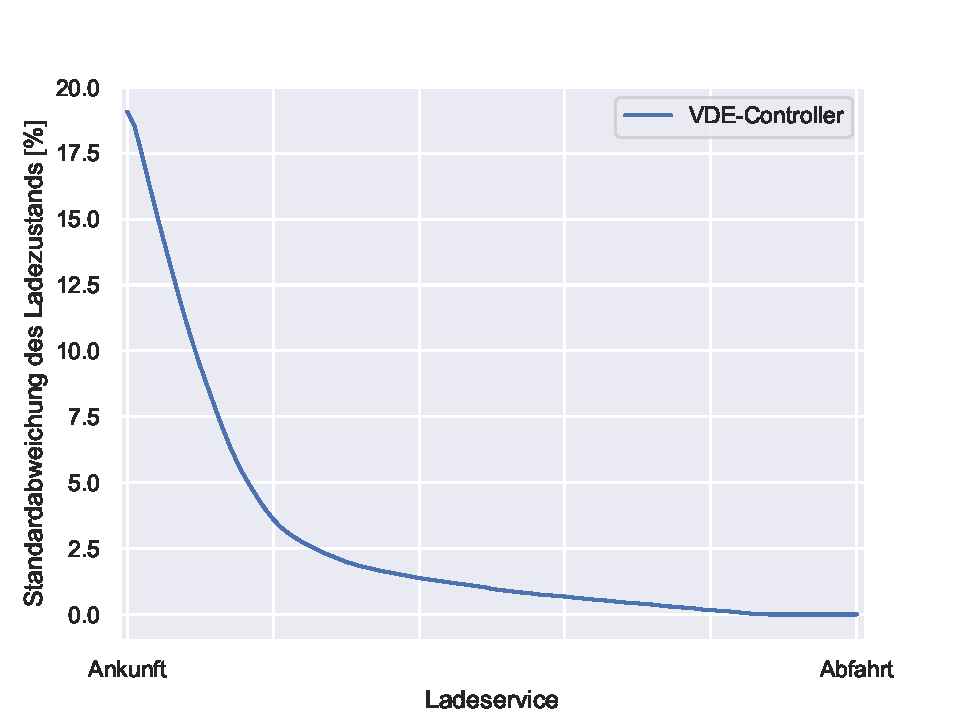
\includegraphics[width=\linewidth]{img/VDE_tau_trafo/tau_VDE_trafo_2_soc_std.pdf}
        \subcaption{Durschschnittliche Standardabweichung des Ladezustandes aller Elektrofahrzeuges über den Verlauf eines Ladeservices}
        \label{ABB_VDETrafo_SocSTD}
	\end{subfigure}
\end{figure}
Abbildung \ref{ABB_VDETrafo_SocMEAN} zeigt dem mittleren Ladestand aller Teilnehmer über den zeitlichen Verlauf der jeweilige Ladeservice. Abbildung \ref{ABB_VDETrafo_SocSTD} zeigt die zugehörige Standardabweichung des Ladestandes ebenfalls über den zeitlichen Verlauf der Ladeservice hinweg. Der schnelle Anstieg des mittleren Ladestandes deutet daraufhin das die Fahrzeuge schnell mit größeren Mengen an Energie versorgt werden können. Die Standardabweichung fällt in ebensolchem Tempo, was den Schluss zulässt, dass viele Fahrzeuge relativ zeitgleich laden können. Die Kurve der Standardabweichung flacht allerdings nach etwa 20 \% des Ladeservices stark ab, in kaum 25 \% der Zeit wird die Standardabweichung um mehr als 15 Prozent reduziert auf etwa 2,5 \%, bis sie jedoch dann auf 0 \% zurückgeht, ist der Ladeservice dann fast abgeschlossen. Diese Tatsache zeigt, dass es trotz der schnellen Abnahme der Standardabweichung dennoch verhältnismäßig lange dauert, bis die Ladeservice als erfolgreich eingestuft werden können.\\
\begin{figure}[htb]
\centering
	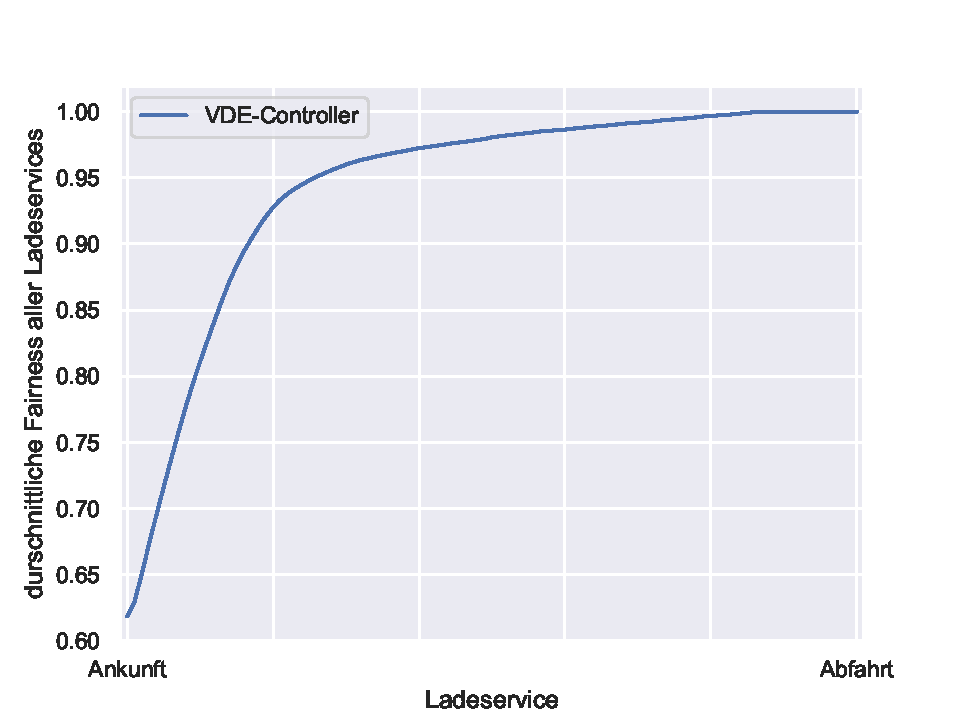
\includegraphics[scale=0.6]{img/VDE_tau_trafo/tau_VDE_trafo_2_qoe.pdf}
	\caption{Durchschnittlicher Qualitätserfahrung aller Elektrofahrzeuges über den Verlauf eines Ladeservices}
	\label{Abb_VDETrafo_Fairness}
\end{figure}

Abbildung \ref{Abb_VDETrafo_Fairness} zeigt die mittlere Fairness der Qualitätserfahrung aller Teilnehmer über den zeitlichen Verlauf ihrer Ladeservice hinweg. Dieser Graph zeigt ein ähnliches Bild wie bereits die Standardabweichung ein schneller Anstieg zu Beginn, dann flacht die Kurve jedoch ab und erst nahe am Ende der Ladeservice wird die Maximale Fairness erreicht. Dieser Verlauf der Kurve weist darauf hin, dass es vielen Teilnehmer gelingt sehr schnell zu Beginn ihres Ladeservices zu laden, es jedoch auch Teilnehmer gibt, welche sehr viel ihrer Zeit nutzen müssen um den Ladeservice erfolgreich abschließen zu können. Dies zeigt wieder Unterschiede zwischen den Fahrzeugen auf.

\subsection{Slotted Aloha mit Teilnehmerzahl mit Transformatorkontroller}
\label{chap_SAparT}
Die Methodik welche den VDE-Controller mit der Teilnehmer basierten Slotted ALOHA Regelung erweitert wurde bereits betrachten, hier werden die Ergebnisse vorgestellt, wird zusätzlich noch der Transformatorkontroller verwendet. Die Methodik wurde ebenfalls über den Zeitraum von einer Woche simuliert. Die Methodik wird hinsichtlich der Transformatorlast, der Spannung, der Teilnehmerzahl, der Kollisionsanzahl, der Quality of Experince und der Fairness untersucht. Bei der Transformatorlast, der Spannung, der Teilnehmerzahl wird nur ein Werktag aus der durchlaufen Woche dargestellt, um eine bessere Übersichtlichkeit der Graphen zu erreichen.\\
\begin{figure}
	\begin{subfigure}{\linewidth}
		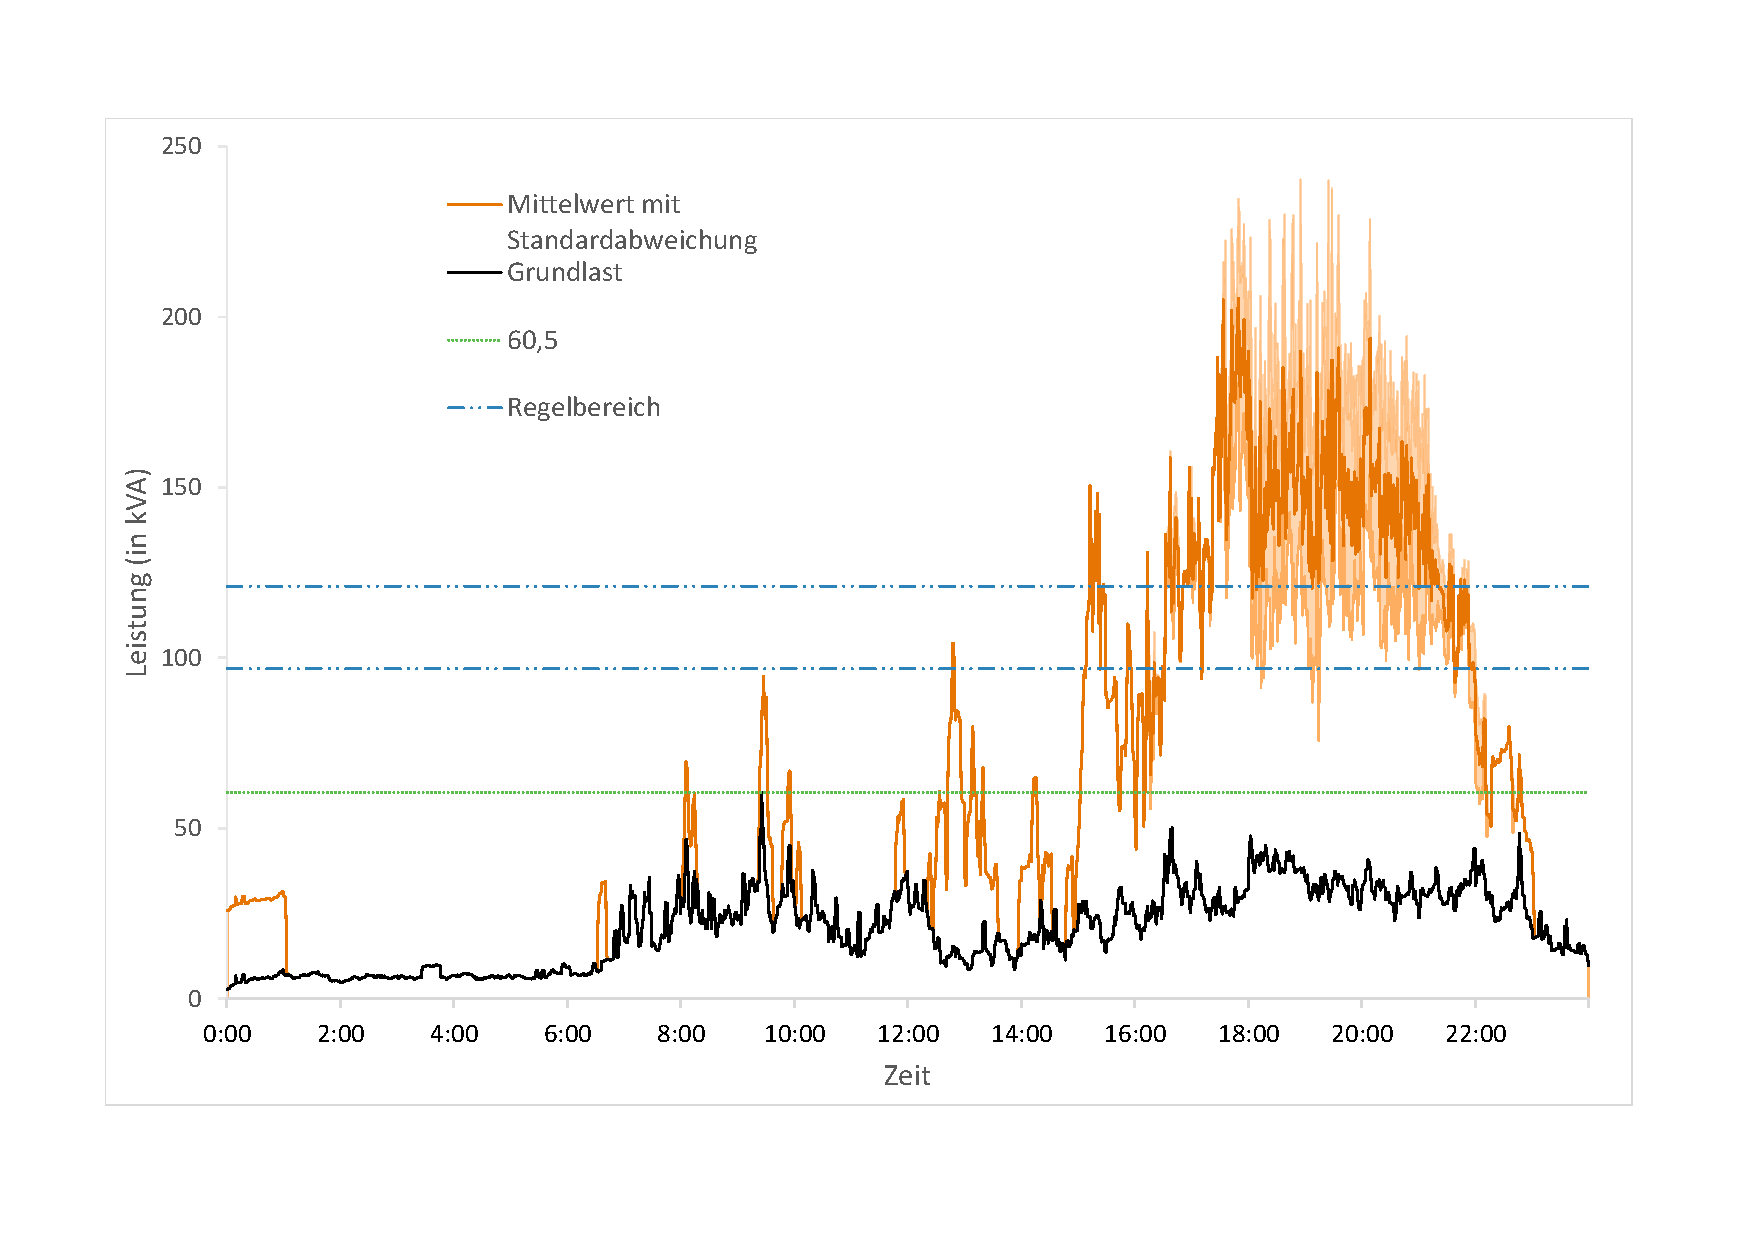
\includegraphics[scale=0.5]{img/SA_par_trafo/TrafoLast3.pdf}
		\caption{Transformatorlast über den Verlauf eines Tages}
		\label{Abb_SAparTrafo_TrafoLast}
	\end{subfigure}
	\begin{subfigure}{\linewidth}
		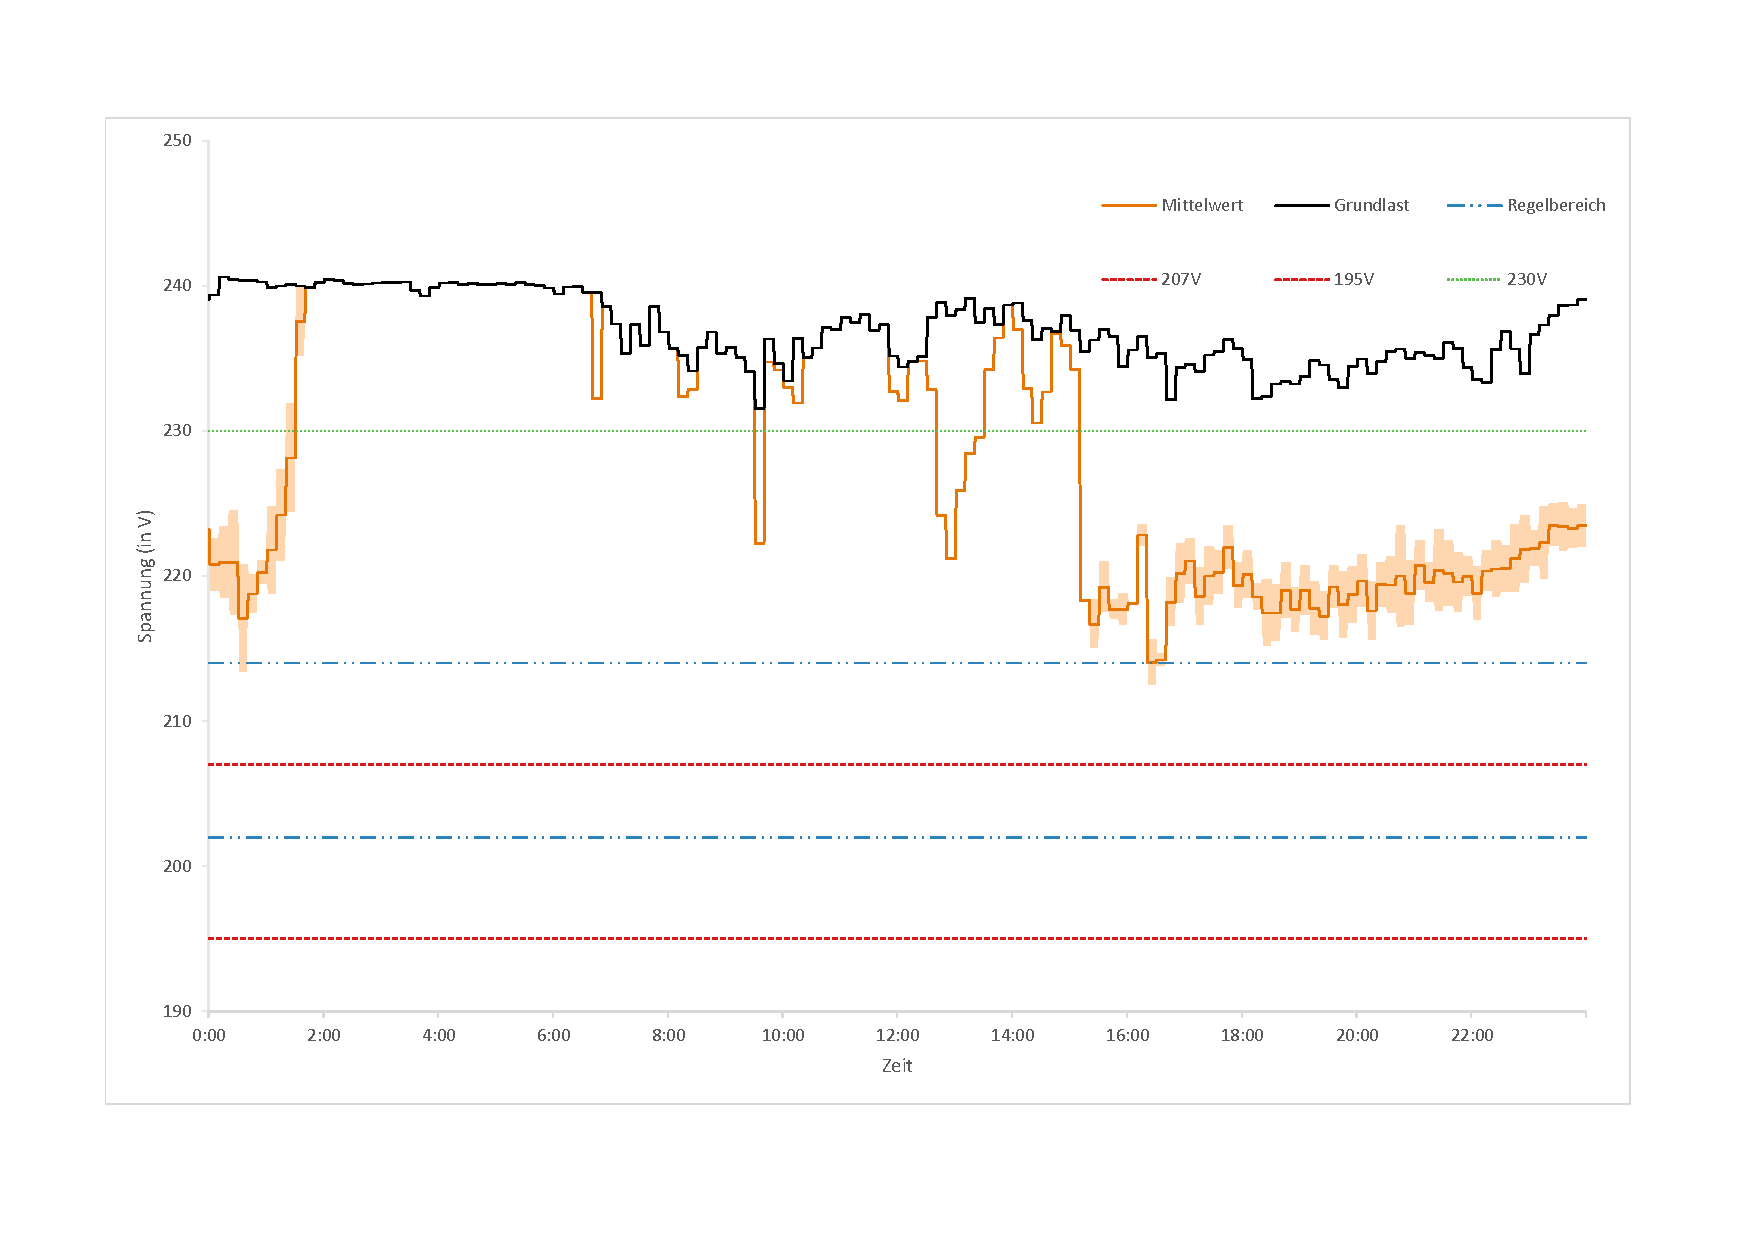
\includegraphics[scale=0.5]{img/SA_par_trafo/Voltage2.pdf}
		\caption{10 Minuten Mittelwerte der Spannung über den Verlauf eines Tages}
		\label{Abb_SaparTrafo_Spannung}
	\end{subfigure}
\end{figure}

Abbildung \ref{Abb_SAparTrafo_TrafoLast} zeigt den Mittelwert der Menge der bezogenen Scheinleistung am Transformator mit der zugehörigen Standardabweichung über den Verlauf eines Tages. Die hier betrachteten Methodik verwendet den Transformatorkontroller, welcher innerhalb der markierten Grenzen arbeitet und bei Messwerten oberhalb des Regelbereiches keinen weiteren Lastbezug zulässt. Am Graphen ist erkennbar wie der Kontroller einen dauerhaften Bezug von mehr als der erlaubten Leistung unterbindet und sich der Mittelwert meist innerhalb des Regelbereiches oder darunter aufhält. Einzelne Spitzen nach oben sind aufgrund der dezentralen Verwendung des Kontrollers nicht zu vermeiden, da die einzelnen Teilnehmer die anderen Teilnehmer nicht berücksichtigen. Die Last bleibt, wenn sie sich im Regelbereich befindet stabil und schwankt verhältnismäßig. Die teils hohe Standardabweichung weist auf große Unterschiede zwischen den absolvierten Durchläufen hin.\\
Abbildung \ref{Abb_SaparTrafo_Spannung} zeigt die Minimalwerte der Mittelwerte der 10 Minuten Intervalle der Spannung über alle Anschlusspunkte hinweg. Neben den eigentlichen Werten wird auch die Standardabweichung über die durchlaufenen Durchgänge mitabgebildet. Die Standardabweichung hier weist auf, im Vergleich zur Transformatorlast, eine höhere Ähnlichkeit der einzelnen Durchläufe hin. Je weiter sich die Messwerte allerdings von der Grundlast entfernen , desto größer wird die Standardabweichung. Anhand des Verlaufs des Graphens ist erkennbar, das die dargestellten Werte nur an wenigen Punkten bis in den Regelbereich des Controllers vordringen. Da nur wenige Werte innerhalb des Regelbereiches liegen, kann der Spannungscontroller auch nur wenig Einfluss nehmen.\\
\begin{figure}[htb]
\centering
	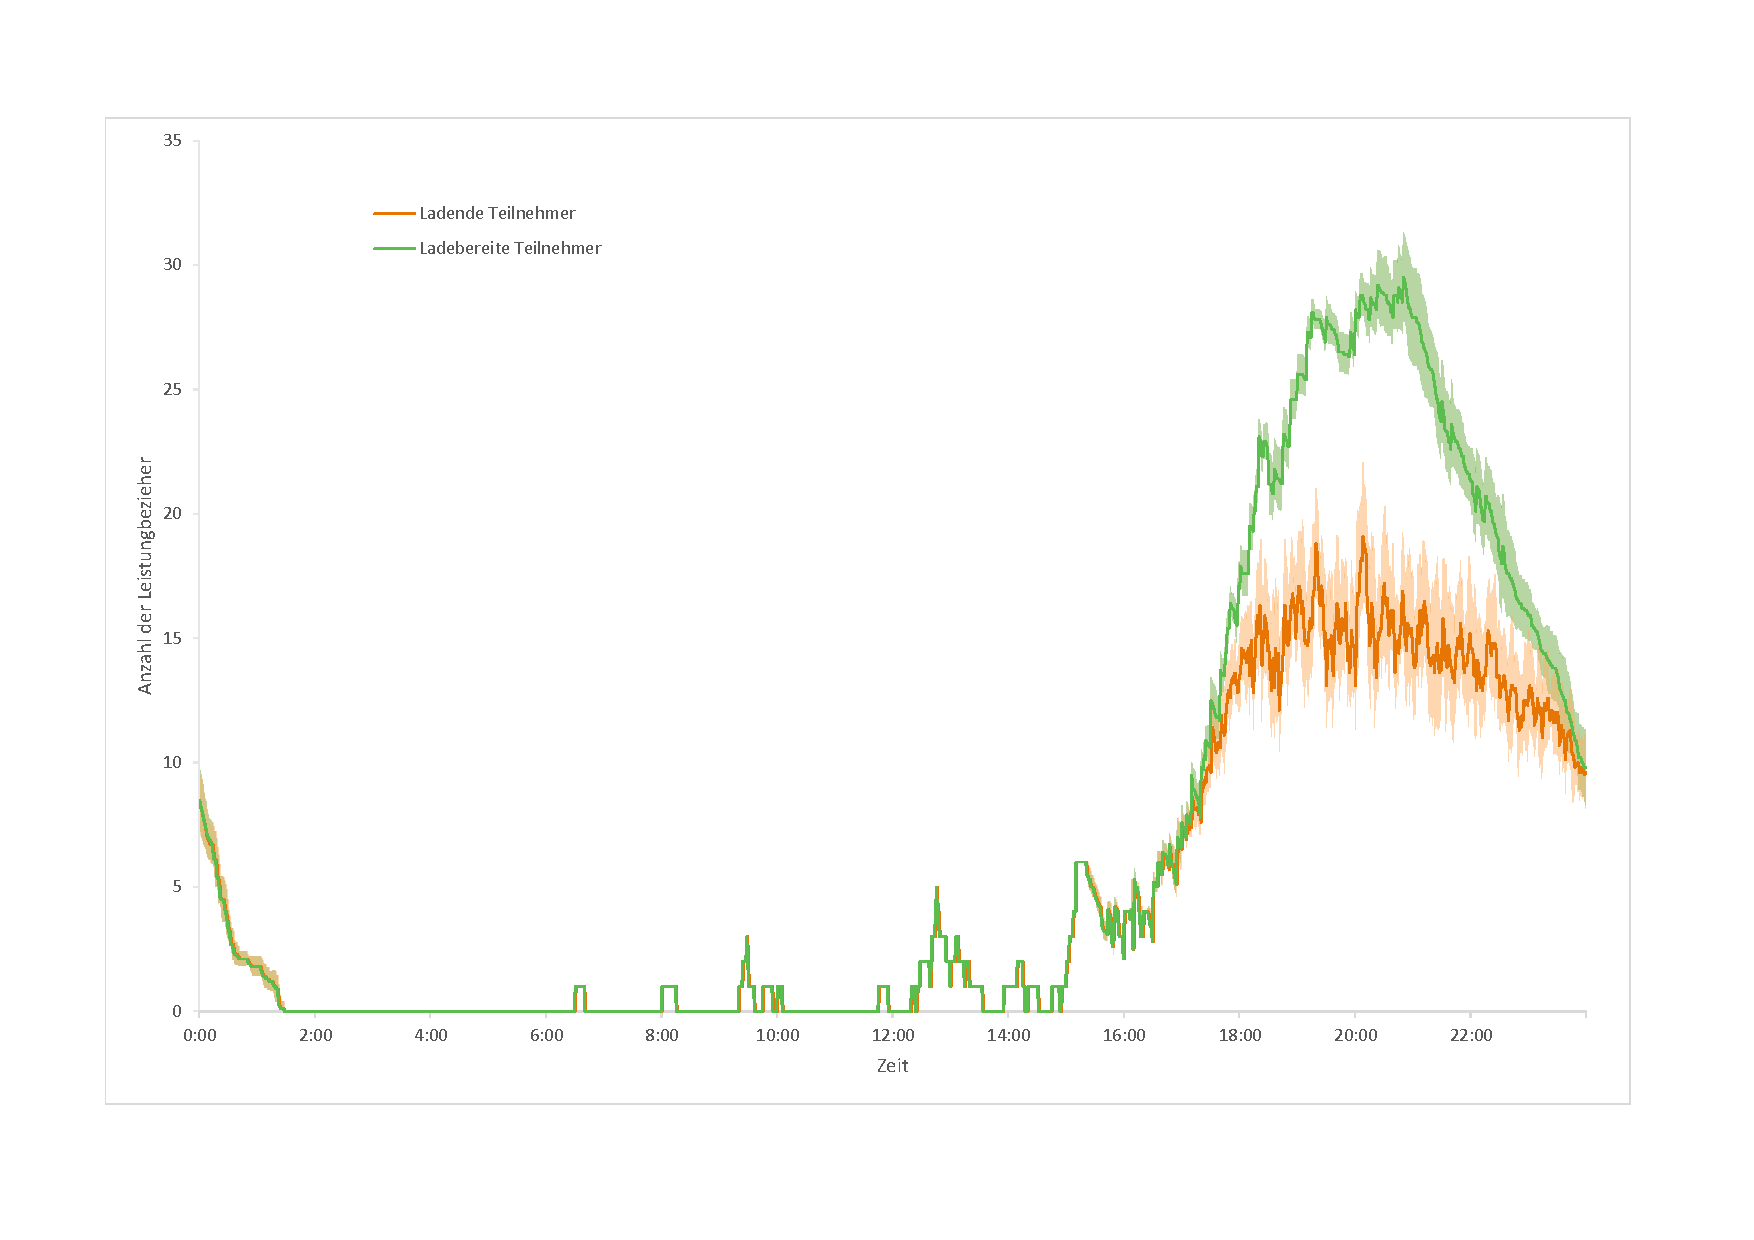
\includegraphics[scale=0.5]{img/SA_par_trafo/Teilnehmer3.pdf}
	\caption{Anzahl der ladebereiten und tatsächlich ladenen Teilnehmer am Niederspannungsnetz über den Verlauf eines Tages}
	\label{Abb_SAparTrafo_Teilnehmer}
\end{figure}
In Abbildung \ref{Abb_SAparTrafo_Teilnehmer} sind die Mittelwerte der Anzahl der ladebereiten und der tatsächlich ladenden Teilnehmer abgebildet. Zu den Graphen selbst wird jeweils noch die jeweils dazugehörige Standardabweichung abgebildet. Die Differenz zwischen der Anzahl an ladebereiten und tatsächlich ladenden Teilnehmern kommt durch das Einhalten der nach einer Kollision berechneten Wartezeit zustande. Die teils schnellen Anstiege der Zahl der ladenden Teilnehmer ohne denselben Anstieg in der Zahl der ladebereiten Teilnehmer weist auf zu ähnliche Wartezeiten hin. Diese zu ähnlichen Wartezeiten helfen der Lastverteilung, die durch das Warten erreicht werden soll, nur bedingt und sollten eigentlich vermieden werden. Da bei dieser Methodik zur Bestimmung der Wartezeit allerdings nur die Zahl der ladebereiten Teilnehmer verwendet wird, gibt es nur sehr beschränkte Auswahlmöglichkeiten und damit auch Überscheidungen bei der Auswahl.\\
Bei zu Beginn des betrachteten Zeitraumes befinden sich bereits Teilnehmer in ihren Ladeservices, was auch die Transformatorauslastung und die Spannungswerte erklärt. Die Teilnehmer schließen die Ladeservice allerdings schnell ab, was die Transformatorlast und die Spannung, auf die Grundlast zurückkommen lasst. In dem Zeitraum von 02:00 bis etwa 15:00 steigen die Werte zwar gelegentlich an, allerdings ist weder das Eingreifen des TransformatorKontrollers noch das des Spannungscontrollers erforderlich. Ab etwa 15:00 steigt die Zahl der ladebereiten Teilnehmer schnell an, was sich auch an der Höher der Transformatorlast und dem Fallen der Spannung erkennen lässt. Ab etwa 18:00 beginnt sich ein deutlicher Unterschied zwischen der Anzahl an ladebereiten Teilnehmer und tatsächlich ladenden Teilnehmern zu zeigen. Die Anzahl der ladenden Teilnehmer hört bei etwa 20 Teilnehmer auf zu steigen, während die Anzahl der ladebereiten Teilnehmer auf mehr als 30 ansteigt. Die eher stabile Zahl an ladenden Teilnehmer zeigt sich auch an der stabilen Transformatorauslastung und den stabilen Messwerten der Spannung. Zum Ende des betrachteten Zeitraumes sinkt Anzahl der Teilnehmer und so sinkt auch die Transformatorlast und die Spannung nähert sich wieder der Grundlast an.\\
Auch für diese Methodik wird die Einhaltung der Norm DIN EN 50160 in Hinsicht auf die Spannungsqualität an Anschlusspunkten des Niederspannungsnetzes untersucht. Im Schnitt über alle Durchgänge mit dieser Methodik wurden keine Unterschreitungen von -10 \% p.u. und keine Unterschreitungen der -15 \% p.u. Marke festgestellt. Somit wurde die Norm erfüllt.
Da hier sowohl der Transformator- als auch der Spannungskontroller verwendet wurde, wird bei dieser Methodik auch auf beide Arten von Kollisionen reagiert. Im Schnitt kam es zu 461,8 (+- 10,4 \%) Spannungskollisionen und zu 6588,7 (+- 1,6 \%) Transformatorkollisionen. Da die Kollisionen auch gemeinsam auftreten können, kam es nur in 6589,3 (+- 1,6 \%) Fällen zu einer Situation in der eine oder beide Kollisionsarten vorlagen. Unterbrechungen von Ladevorgängen durch Kollisionen gab es lediglich in 3084,0 (+- 0,7 \%) Fällen. Das bedeutet in weniger als der Hälfte der Fälle; wo eine Kollision aufgetreten ist, musste auch darauf reagiert werden.\\
In dem betrachteten Simulationszeitraum von einer Woche wurden 557 Ladeservices gestartet, es konnten allerdings im Schnitt nur 554,1 Services erfolgreich abgeschlossen werden, also mussten durchschnittlich 2,9 Mal (+- 42 \%) Ladeservices beendet werden, bevor die Batterie des Fahrzeuges auf 100 \% geladen werden konnte. Die Standardabweichung des Ladestandes beim Verlassen der Ladestation lag nur bei etwa 0,43 \% (+- 39,5 \%), der Mittelwert des Ladezustandes bleibt davon allerdings unverändert bei 100 \% wenn die Ladestation verlassen wird. Der Mittelwert und die Standardabweichung des Ladestandes sind in Abbildung \ref{ABB_SAparTrafo_SocMEAN} bzw. \ref{ABB_SAparTrafo_SocSTD} angetragen.\\
\begin{figure}
	\begin{subfigure}{0.49\linewidth}
		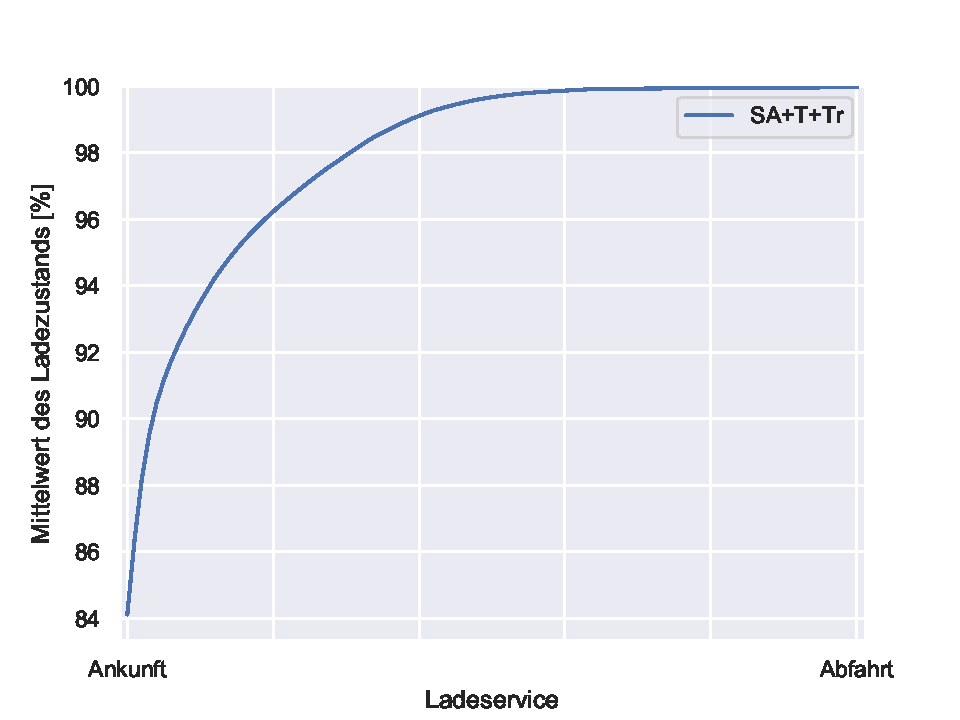
\includegraphics[width=\linewidth]{img/SA_par_trafo/SlottedAloha_participants_VDE_tau_trafo_15_soc_mean.pdf}
        \subcaption{Durchschnittlicher Ladezustand aller Elektrofahrzeuges über den Verlauf eines Ladeservices}
        \label{ABB_SAparTrafo_SocMEAN}
	\end{subfigure}
	\begin{subfigure}{0.49\linewidth}
		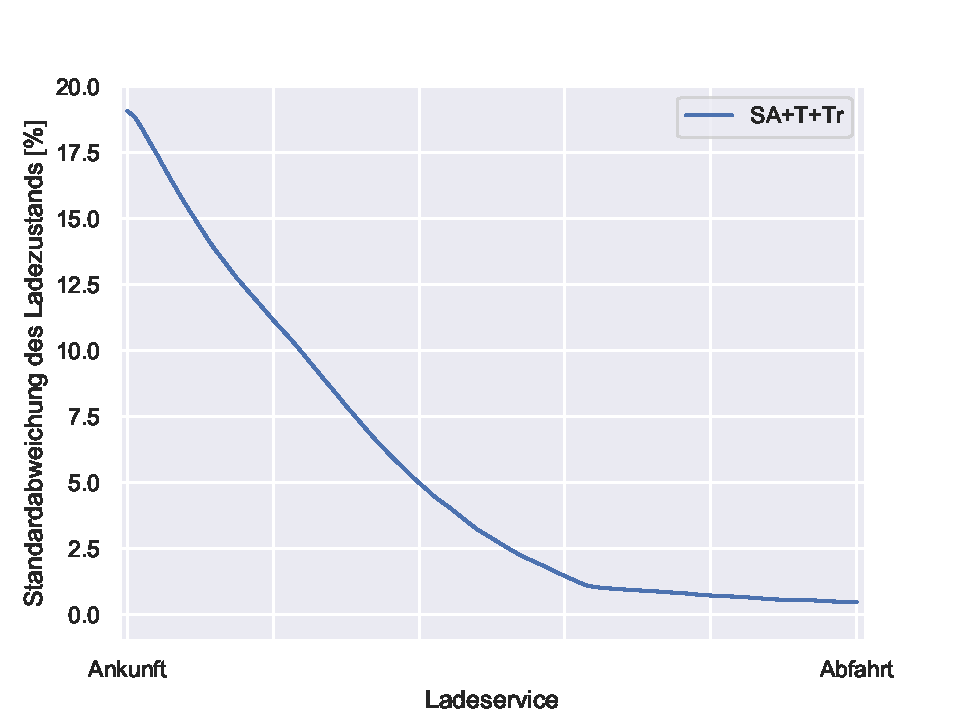
\includegraphics[width=\linewidth]{img/SA_par_trafo/SlottedAloha_participants_VDE_tau_trafo_15_soc_std.pdf}
        \subcaption{Durschschnittliche Standardabweichung des Ladezustandes aller Elektrofahrzeuges über den Verlauf eines Ladeservices}
        \label{ABB_SAparTrafo_SocSTD}
	\end{subfigure}
\end{figure}
Abbildung \ref{ABB_SAparTrafo_SocMEAN} Zeigt den mittleren Ladestand aller Fahrzeuge über den zeitlichen Verlauf der Ladeservice hinweg. Abbildung \ref{ABB_SAparTrafo_SocSTD} zeigt die gemittelte Höhe der Standardabweichung des Ladezustandes über alle Ladeservices im zeitlichen Verlauf. Trotz der verbleibenden Standardabweichung zum Ende der Ladeservice hin, zeigt Abbildung \ref{ABB_SAparTrafo_SocMEAN} 100 \% mittleren Ladezustand an. Der Wechsel der  Abnahme der Standardabweichung bei etwa 60 \% der Zeit weisen daraufhin, das viele Ladevorgänge bis dahin abgeschlossen sind, die die es nicht sind allerdings nur noch sehr langsam ihren Ladestand erhöhen können. \\
\begin{figure}[htb]
\centering
	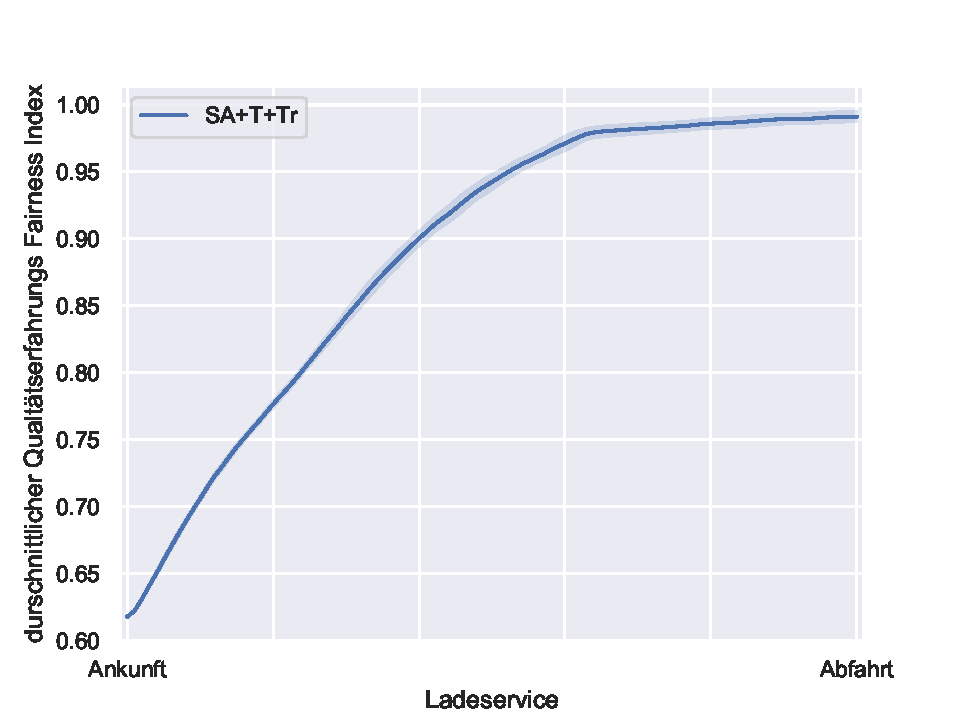
\includegraphics[scale=0.6]{img/Sa_par_trafo/SlottedAloha_participants_VDE_tau_trafo_15_qoe.pdf}
	\caption{Durchschnittlicher Qualitätserfahrung aller Elektrofahrzeuges über den Verlauf eines Ladeservices}
	\label{Abb_SAparTrafo_Fairness}
\end{figure}
Abbildung \ref{Abb_SAparTrafo_Fairness} zeigt den Mittelwert der Fairness über alle Teilnehmer hinweg. Die Fairness bestimmt sich über die Standardabweichung, da diese hier nicht 0 wird, wird auch die Fairness nicht maximal. Da nicht alle Teilnehmer in der Lage waren ihre Ladeservice erfolgreich abzuschließen, erreicht auch der Wert der Qualitätserfahrung nicht das Maximum, im Mittel über alle Durchläufe konnte eine Qualitätserfahrung von 0,99 von 1 erreicht werden. Die Fehlende Qualitätserfahrung spiegelt sich auch in der Fairness wider, welch zwar hoch wird, jedoch wird auch hier das Maximum nicht erreicht. Auch am Graphen der Fairness zeigt sich ein Bild wie bei der Standardabweichung des Ladestandes. Bis etwa 60 \% durch die Ladeservice steigt der Graph gleichmäßig an, ab dann steigt der Graph allerdings nur noch sehr gering weiter an. 

\subsection{Slotted Aloha mit Teilnehmerzahl und Fahrzeugparametern mit Transformatorkontroller}
\label{chap_SAwtT}
Die Methodik, welche bei der Erweiterung des VDE-Controllers um die Slotted Aloha Regelung neben der Teilnehmerzahl auch Fahrzeugparameter verwendet wurde ebenfalls noch um den Transformatorkontroller erweitert. Auch diese Konfiguration wurde über den Zeitraum von einer Woche hinweg simuliert. Sie wird hinsichtlich der Transformatorlast, der Spannung, der Teilnehmerzahl, der Kollisionsanzahl, der Quality of Experince und der Fairness untersucht. Bei der Transformatorlast, der Spannung, der Teilnehmerzahl wird erneut nur ein Werktag aus der durchlaufenen Woche dargestellt, um eine bessere Übersichtlichkeit der Graphen zu erreichen.\\
\begin{figure}
	\begin{subfigure}{\linewidth}
		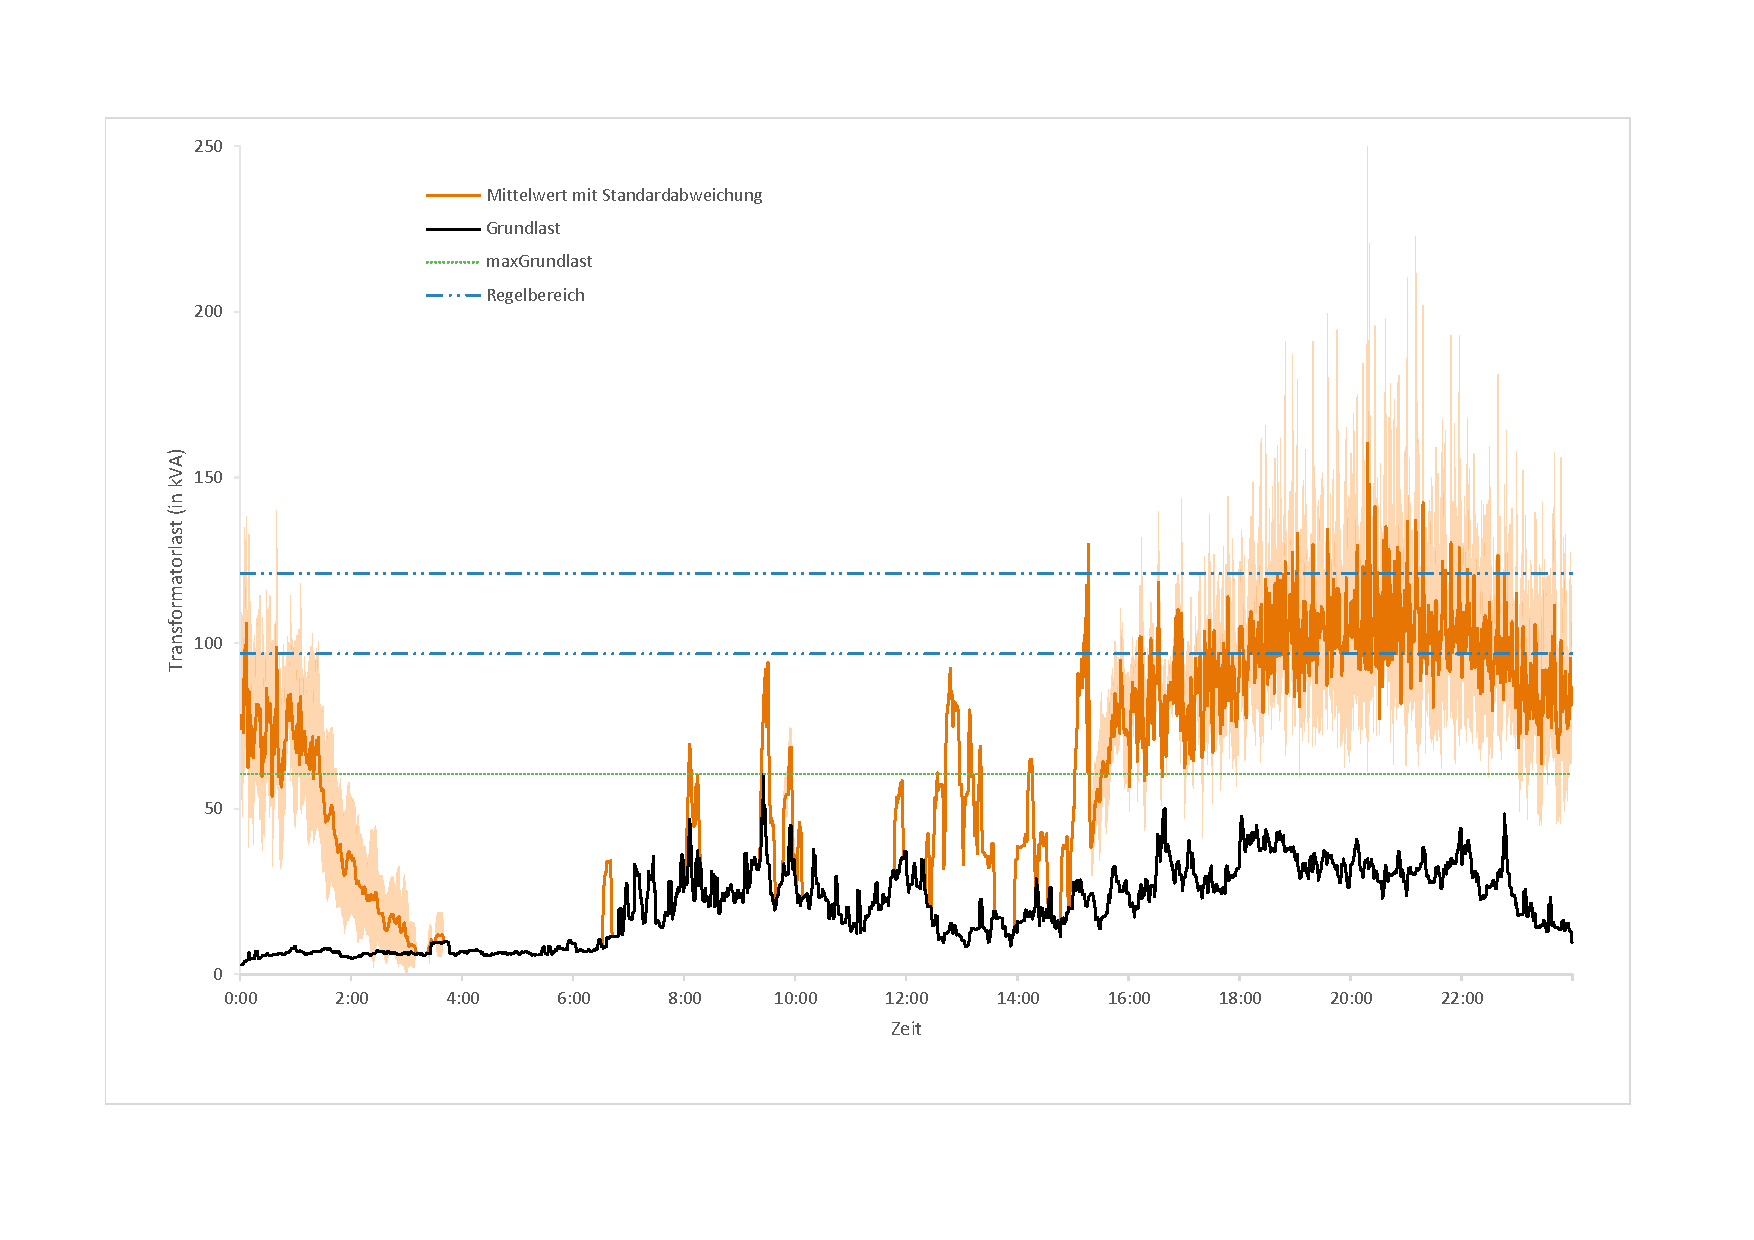
\includegraphics[scale=0.5]{img/SA_wT_trafo/TrafoLast.pdf}
		\caption{Transformatorlast über den Verlauf eines Tages}
		\label{Abb_SAwtTrafo_TrafoLast}
	\end{subfigure}
	\begin{subfigure}{\linewidth}
		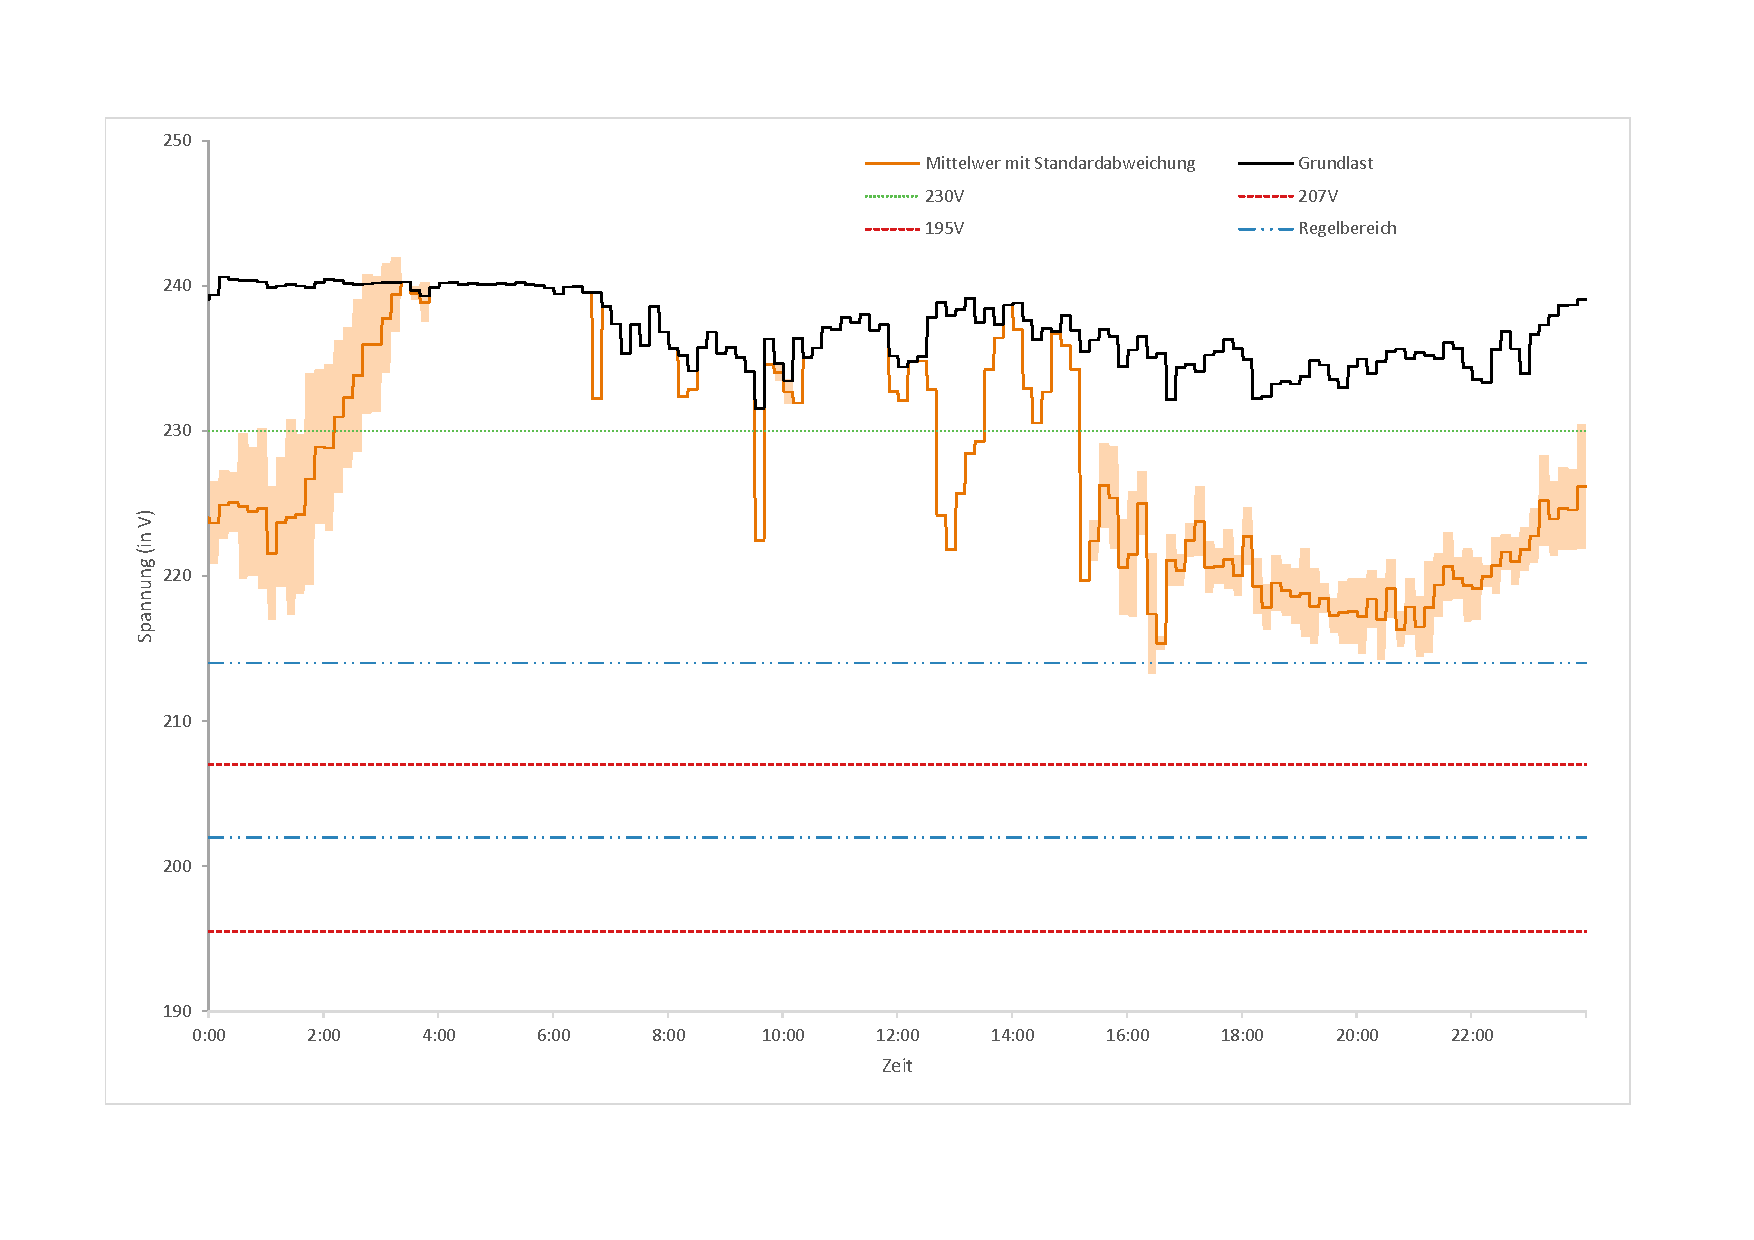
\includegraphics[scale=0.5]{img/SA_wT_trafo/Spannung.pdf}
		\caption{10 Minuten Mittelwerte der Spannung über den Verlauf eines Tages}
		\label{Abb_SAwtTrafo_Spannung}
	\end{subfigure}
\end{figure}
Abbildung \ref{Abb_SAwtTrafo_TrafoLast} zeigt den Mittelwert der Scheinleistung, welche am Transformator ins Niederspannungsnetz abgegeben wurde, mit der dazugehörigen Standardabweichung über den Verlauf eines Tages. Auch hier wird der Transformatorkontroller verwendet, welcher innerhalb der markierten Grenzen arbeitet und bei Messwerten oberhalb des Regelbereiches keinen weiteren Lastbezug zulässt. Die teils hohe Standardabweichung deutet auf unterschiedliche Ergebnisse der einzelnen Durchläufe hin. Bis auf einige Ausbrüche nach oben, welche sich aufgrund des dezentralen Verhaltens des Kontrollers nicht vermeiden lassen, bleiben die Werte des Graphen im oder unter dem Regelbereich des Kontrollers. Wenn sich die Menge der bezogenen Leistung am oder im Lastbereich befindet, schwanken die Werte zwar, allerdings in einem vertretbaren den Umständen entsprechenden Rahmen.\\
In Abbildung \ref{Abb_SAwtTrafo_Spannung} sind die Mittelwerte der minimalen 10 Minuten Mittelwerte der Spannung angetragen, ebenso wie die zugehörige Standardabweichung. Die Werte weisen teils eine hohe Standardabweichung auf, was auf größere Unterschiede zwischen den einzelnen Durchläufen hindeutet. Wie bereits bei der vorhergehenden Methodik, welche ebenfalls den Trafokontroller verwendet, liegen kaum Werte innerhalb des Regelbereiches des Spannungskontrollers. Somit lässt auch hier feststellen, wenn wenig Werte im Regelbereich des Kontrollers liegen, kann der Kontroller auch nur bedingt eingreifen und hat somit bei dieser Methodik wenig Einfluss auf das Ergebnis.\\
\begin{figure}[htb]
\centering
	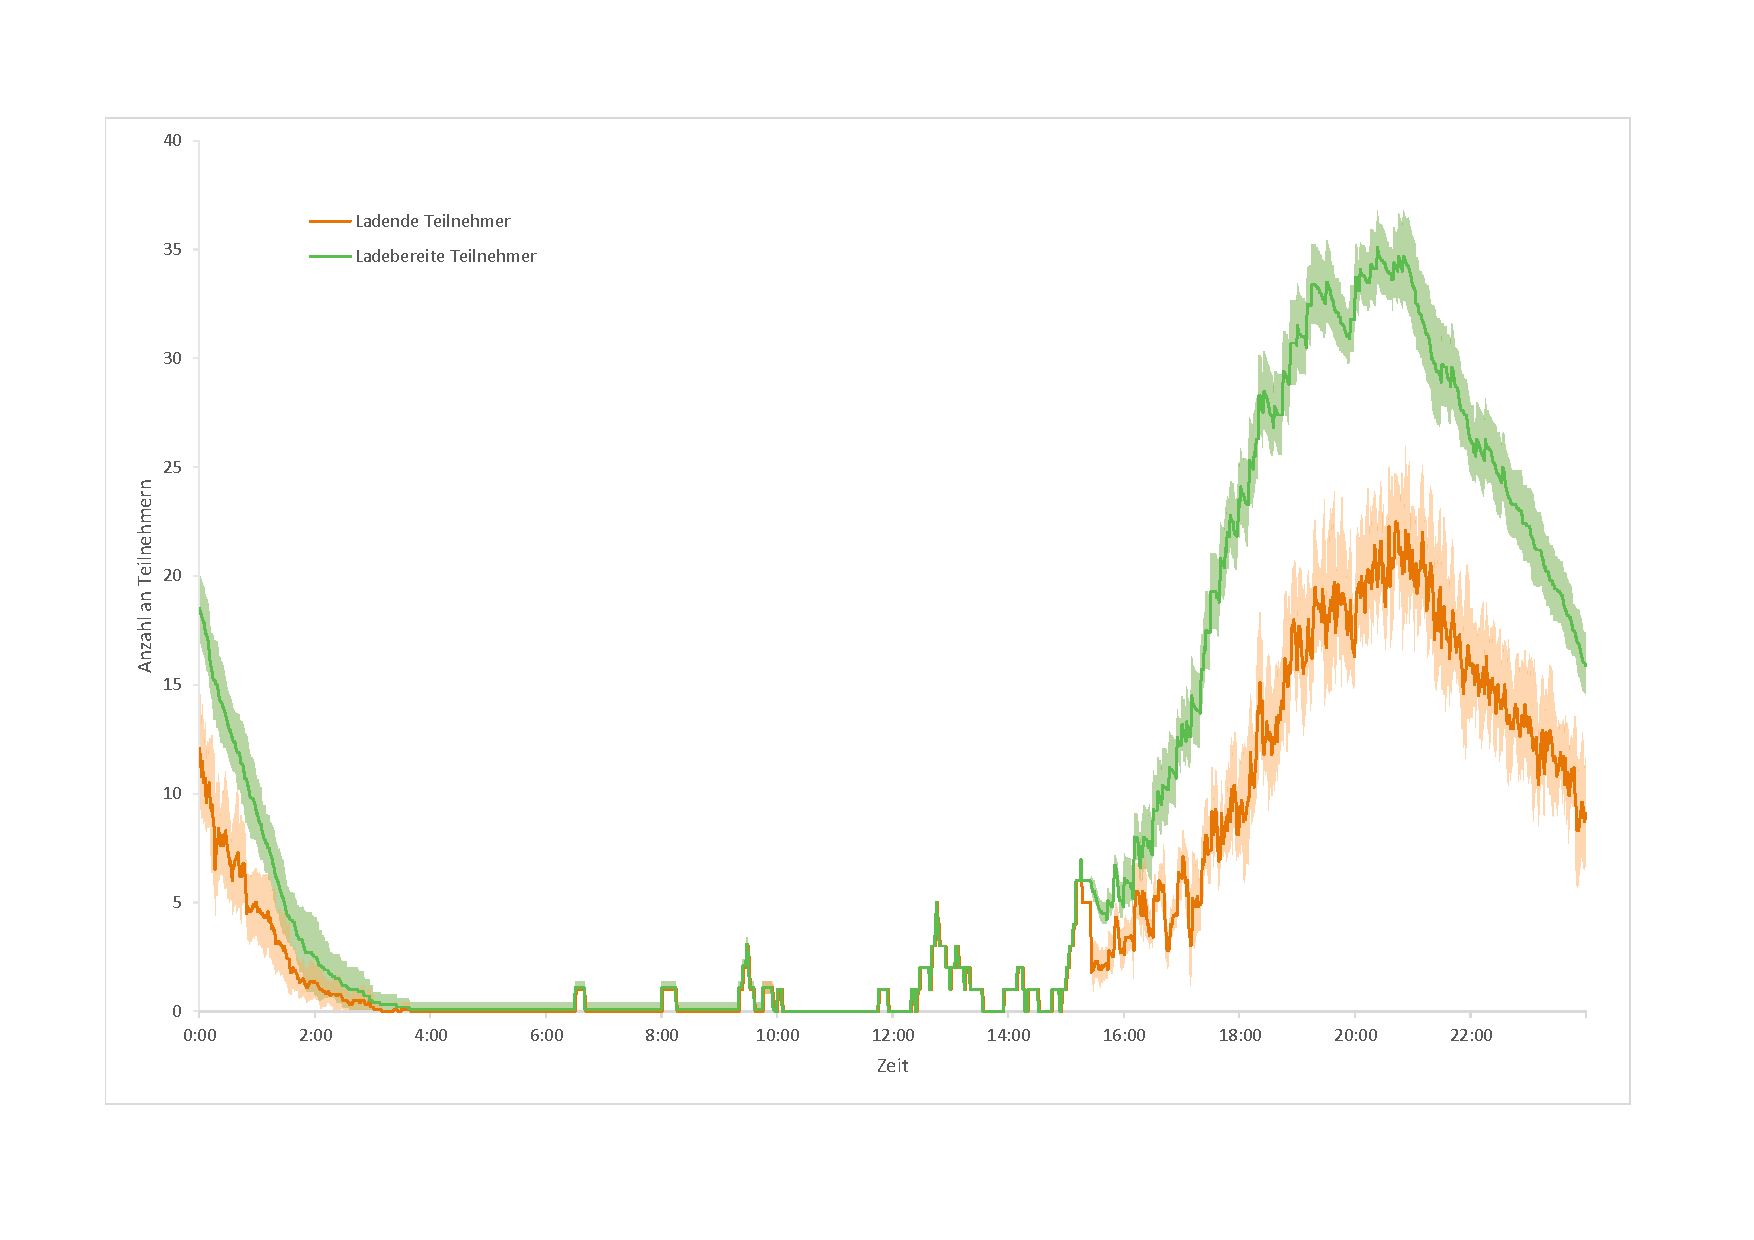
\includegraphics[scale=0.5]{img/SA_wT_trafo/Teilnehmer.pdf}
	\caption{Anzahl der ladebereiten und tatsächlich ladenen Teilnehmer am Niederspannungsnetz über den Verlauf eines Tages}
	\label{Abb_SAwtTrafo_Teilnehmer}
\end{figure}

Abbildung \ref{Abb_SAparTrafo_Teilnehmer} zeigt die mittlere Anzahl der ladebereiten und tatsächlich ladenden Teilnehmer am Niederspannungsnetz mit den zugehörigen Standardabweichungen. Der Unterschied zwischen den beiden Kurven kommt durch die Vergabe von Wartezeiten zustande, in denen nicht geladen werden kann. Die beiden Kurven haben dieselbe grundlegende Form, während des Verlauf, der beiden Kurven, schwanken die Kurven nur in kleinen Intervallen um die Form der Kurve herum. Je kleiner die Standardabweichung der einzelnen Kurven wird, desto näherer kommen sich die beiden Kurven, allerdings werden dabei auch die Werte an sich geringer. Dadurch lässt sich nur schließen, dass die Ergebnisse der Wartezeitbestimmung starken Einfluss auf das Aussehen dieser Kurven haben.\\
Wie bereits bei der andern Methodik mit dem Transformatorkontroller befinden sich zu Beginn des Tages noch Teilnehmer in Ladeservices, diese werden allerdings zügig abgeschlossen und ab etwa 03:00 habe all diese Teilnehmer ihre Ladeservices abgeschlossen. In dem Zeitraum von etwa 03:00 bis etwa 15:00 treten weder Spannungswerte noch Transformatorwerte, welche in dem jeweiligen Regelbereich liegen, folglich wird in diesem Zeitraum keiner der beiden Kontroller aktiv. Nach 15:00 beginnt die Anzahl der ladebereiten Teilnehmer zu steigen, so steigt auch die Anzahl der ladenden Teilnehmer mit an, wodurch die Transformatorlast steigt und die Spannungswerte zu sinken beginnen. Die Transformatorlast steigt mit der wachsenden Anzahl an ladenden Teilnehmern zunächst immer weiter an, wird allerdings durch den Transformatorkontroller begrenzt und dadurch steigt auch die Anzahl an ladenden Fahrzeug nur bis zu einem gewissen Punkt. An allen drei Graphen ist der Punkt der stärksten Auslastung erkennbar, ab etwa 21:00 beginnen sich die Werte wieder zu bessern. An der Höhe der Kurven ist allerdings erkennbar, dass Ladeservices über das Ende des betrachteten Tages hinaus noch andauern. Zu diesem Zeitpunkt befinden sich allerdings weder Transformatorlast noch Spannung noch Im jeweiligen Regelbereich.\\
Auch die Ergebnisse dieser Methodik wurden gemäß der Einhaltung der Norm DIN EN 50160 betrachtet. Es wurden über alle absolvierten Durchläufe hinweg keinerlei Unterschreitungen der Grenzwerte festgestellt, der Grenzwert von -10 \% p.u. wurde zu keinem Zeitpunkt verletzt, somit wurde auch der Grenzwert bei -15 \% p.u. nicht verletzt. Da keinerlei Verletzungen der Grenzwerte Festgestellt wurden, wurde die Norm erfüllt.\\
Bei der hier betrachteten Methodik wird sowohl auf Spannungskollisionen und auch auf Transformatorkollisionen reagiert. Im Schnitt traten 573,8 (+- 15,5 \%) Situation ein, wo ein zu niedrige Spannung gemessen wurde und durchschnittlich 7076,1 (+- 4,3 \%) Situationen, wo eine zu hohe Transformatorlast gemessen wurde. Da beide Arten dieser Situation zeitgleich auftreten können, kam es im Schnitt zu 7077 (+- 4,3 \%)Situationen in denen eine Kollision auftreten könnte. Tatsächlich ist jedoch nur in durchschnittlich 2482,3 (+- 2,5 \%) eine Kollision aufgetreten und eine Wartezeit wurde berechnet. Bei 1108800 betrachteten Situation traten im Schnitt lediglich 2482,5 Kollisionen auf, was einem Anteil von 0,22 \% der betrachteten Situationen entspricht. Dir geringe Anzahl an berechneten Wartezeiten bedeutet, das die berechneten Wartezeiten effektiv bestimmt wurden und ihren angedachten Zweck, nämlich weitere Kollisionen zu verhindern, erfüllt haben.\\
Alle im Simulationszeitraum von einer Woche gestarteten Ladeservice wurden erfolgreich abgeschlossen, somit ist die Qualität der Ladeservice maximal. Abbildung \ref{ABB_SAwtTrafo_SocMEAN} zeigt den mittleren Ladestand aller Fahrzeuge über Verlauf der jeweiligen Ladeservice hinweg, Abbildung \ref{ABB_SAwtTrafo_SocSTD} zeigt die dazugehörige Standardabweichung.\\
\begin{figure}
	\begin{subfigure}{0.49\linewidth}
		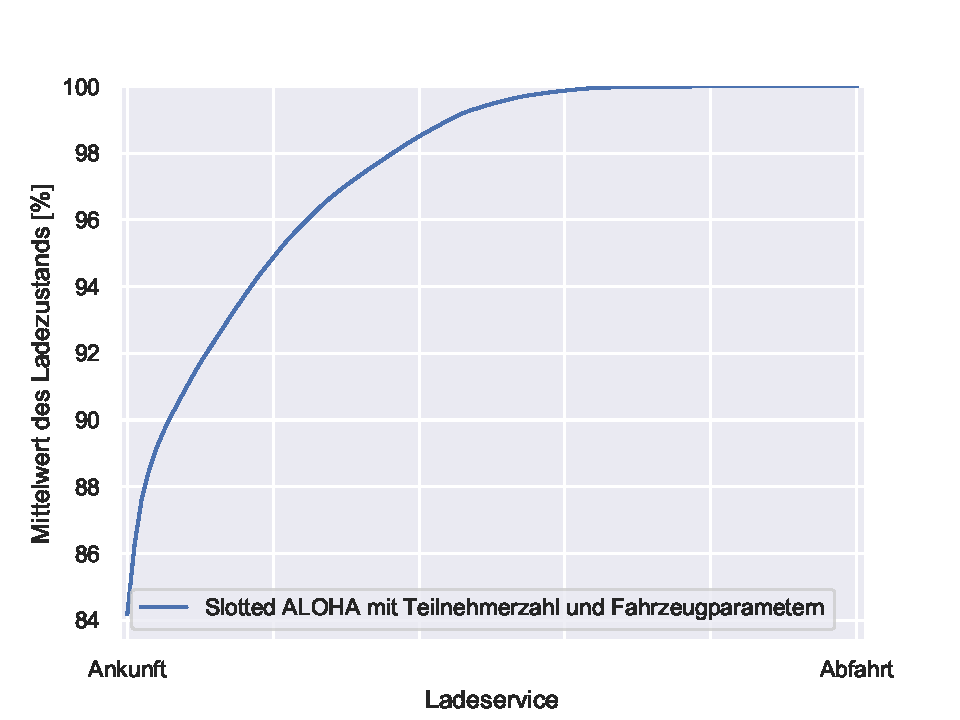
\includegraphics[width=\linewidth]{img/SA_wt_trafo/SlottedAloha_waitingTime_VDE_tau_trafo_13_soc_mean.pdf}
        \subcaption{Durchschnittlicher Ladezustand aller Elektrofahrzeuges über den Verlauf eines Ladeservices}
        \label{ABB_SAwtTrafo_SocMEAN}
	\end{subfigure}
	\begin{subfigure}{0.49\linewidth}
		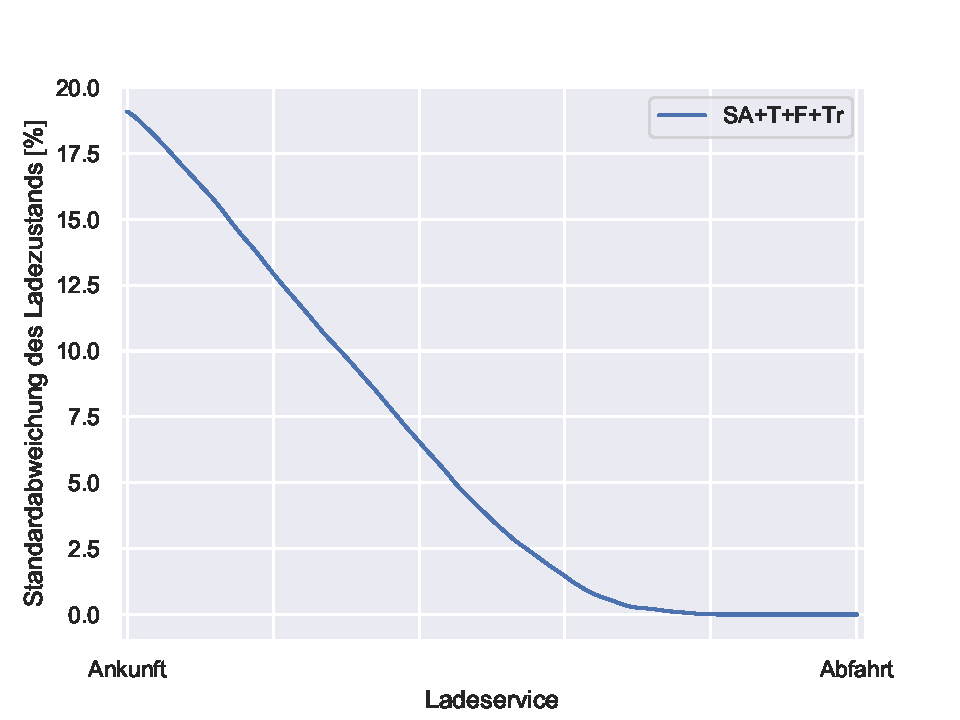
\includegraphics[width=\linewidth]{img/SA_wT_trafo/SlottedAloha_waitingTime_VDE_tau_trafo_13_soc_std.pdf}
        \subcaption{Durschschnittliche Standardabweichung des Ladezustandes aller Elektrofahrzeuges über den Verlauf eines Ladeservices}
        \label{ABB_SAwtTrafo_SocSTD}
	\end{subfigure}
\end{figure}
Den beiden Abbildungen ist zu entnehmen, dass in Schnitt nach 70 \% der Zeit eines Ladeservices der Ladeservice als erfolgreich eingestuft werden kann, da der Ladestand auf 100 \% angestiegen ist und die Standardabweichung des Ladestandes auf 0 \% gefallen ist. Die Standardabweichung sinkt langsamer als der Ladestand steigt, was darauf hindeutet, dass durch die besser gewählten Wartezeiten, die Fahrzeuge besser zeitlich verteilt werden, wodurch die Unterschiede im Ladestand länger bestehen bleiben.\\
\begin{figure}[htb]
\centering
	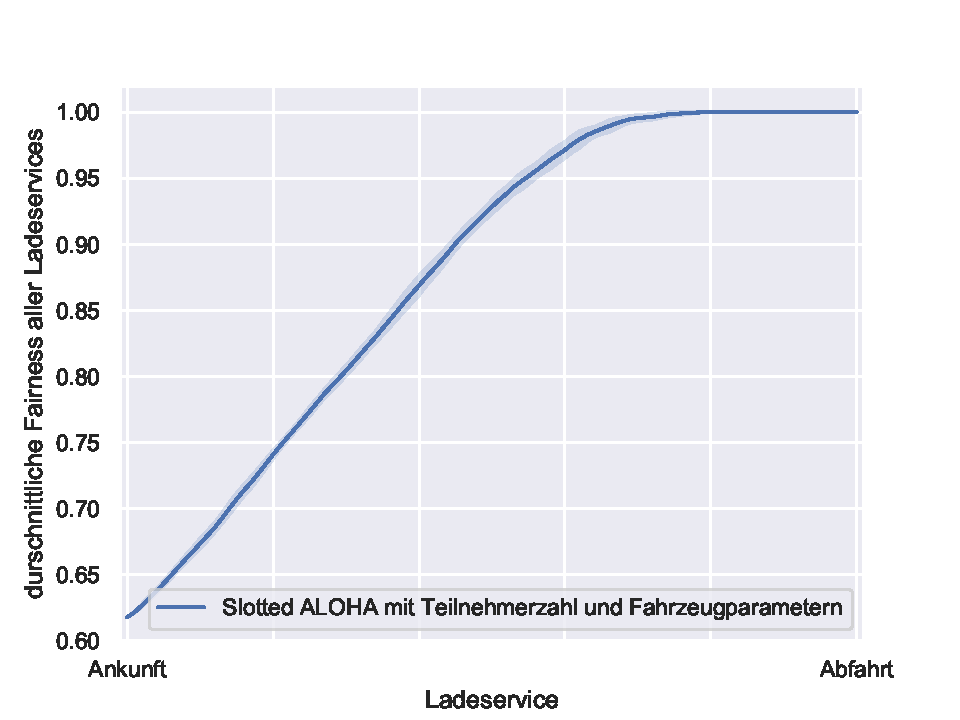
\includegraphics[scale=0.6]{img/Sa_wT_trafo/SlottedAloha_waitingTime_VDE_tau_trafo_13_qoe.pdf}
	\caption{Durchschnittlicher Qualitätserfahrung aller Elektrofahrzeuges über den Verlauf eines Ladeservices}
	\label{Abb_SAwtTrafo_Fairness}
\end{figure}
Abbildung \ref{Abb_SAwtTrafo_Fairness} zeigt die gemittelte Fairness aller Teilnehmer über den zeitlichen Verlauf der Ladeservice hinweg mit der zugehörigen Standardabweichung. Die geringe Standardabweichung weist auf ähnliche Werte, über alle Durchläufe hinweg, hin. Die Fairness steigt an wie die Standardabweichung des Ladestandes fällt. Die Fairness steigt beständig an, bis der Wert bei nach etwa 75 \% der Zeit der Ladeservices maximal wird und auf diesem Niveau bleibt. Die Fairness steigt hier langsamer als bei anderen Methoden, erreicht jedoch trotzdem den maximal möglichen Wert.

\section{Analyse und Auswertung}
\subsection{Vergleich der Varianten ohne Transformatorkontroller}
Es werden nun die drei Methodiken miteinander verglichen, welche keinen Transformatorkontroller verwenden. Diese drei Techniken wurden in den Kapiteln \ref{chap_VDE}, \ref{chap_SApar}, \ref{chap_SAwt} jeweils einzeln für sich analysiert, nun folgt ein Vergleich und eine Analyse über alle drei Varianten hinweg. Betrachtet werden dieselben Parameter wie bei den Einzelanalysen, die Transformatorlast, die Mittelwerte von 10 Minuten Intervallen der Spannung, sowie die Teilnehmerzahl. Auch die Qualität der Ladevorgänge und die Fairness wird über alle drei Methodiken verglichen.
Bei der Transformatorlast, dem Spannungsverlauf und der Anzahl der Teilnehmer wird, wie bereits bei den Einzelanalysen, nur ein Tag des Simulationszeitraums von einer Woche dargestellt, verwendet wird derselbe Werktag wie bisher.
\begin{figure}
	\begin{subfigure}{\linewidth}
		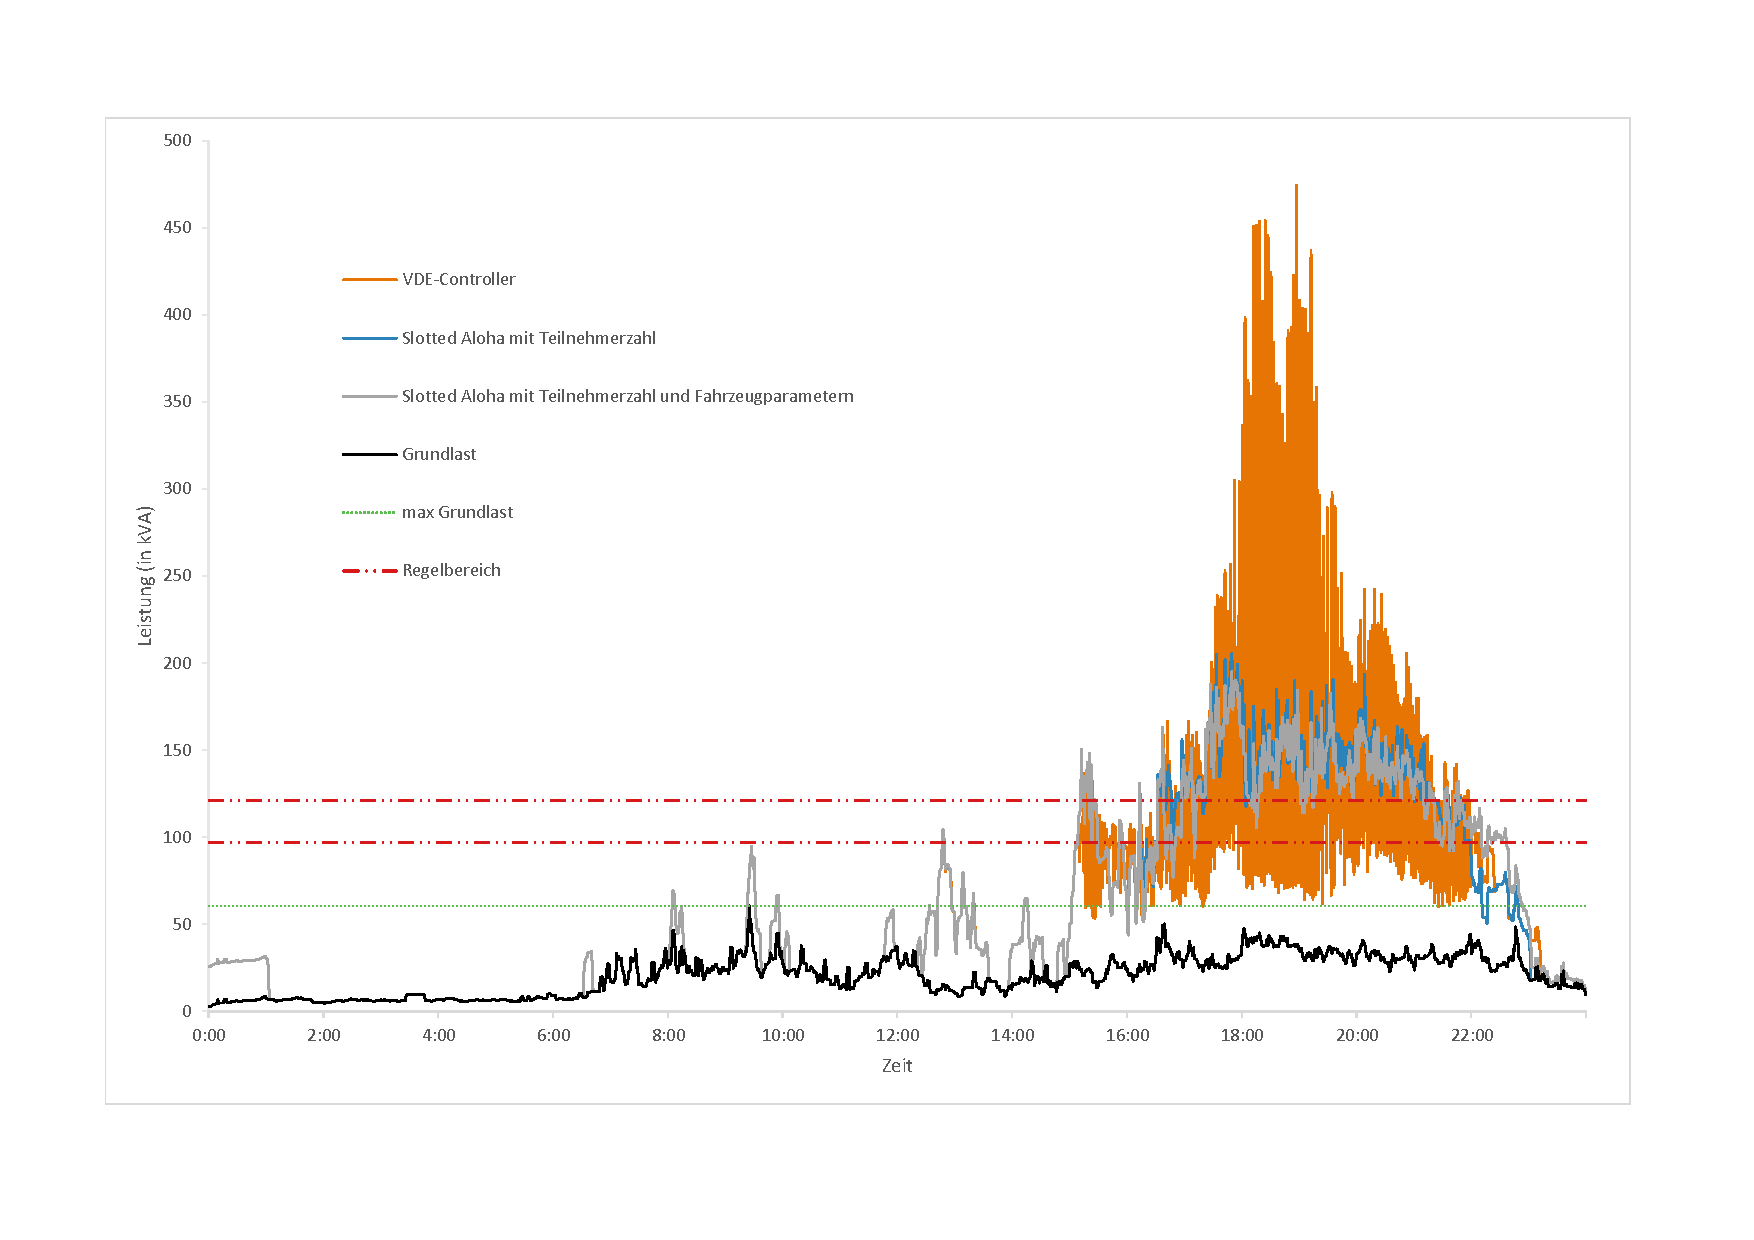
\includegraphics[scale=0.5]{img/ohneTrafo/TrafoLast4.pdf}
		\caption{Transformatorlast über den Verlauf eines Tages}
		\label{Abb_oT_TrafoLast}
	\end{subfigure}
	\begin{subfigure}{\linewidth}
		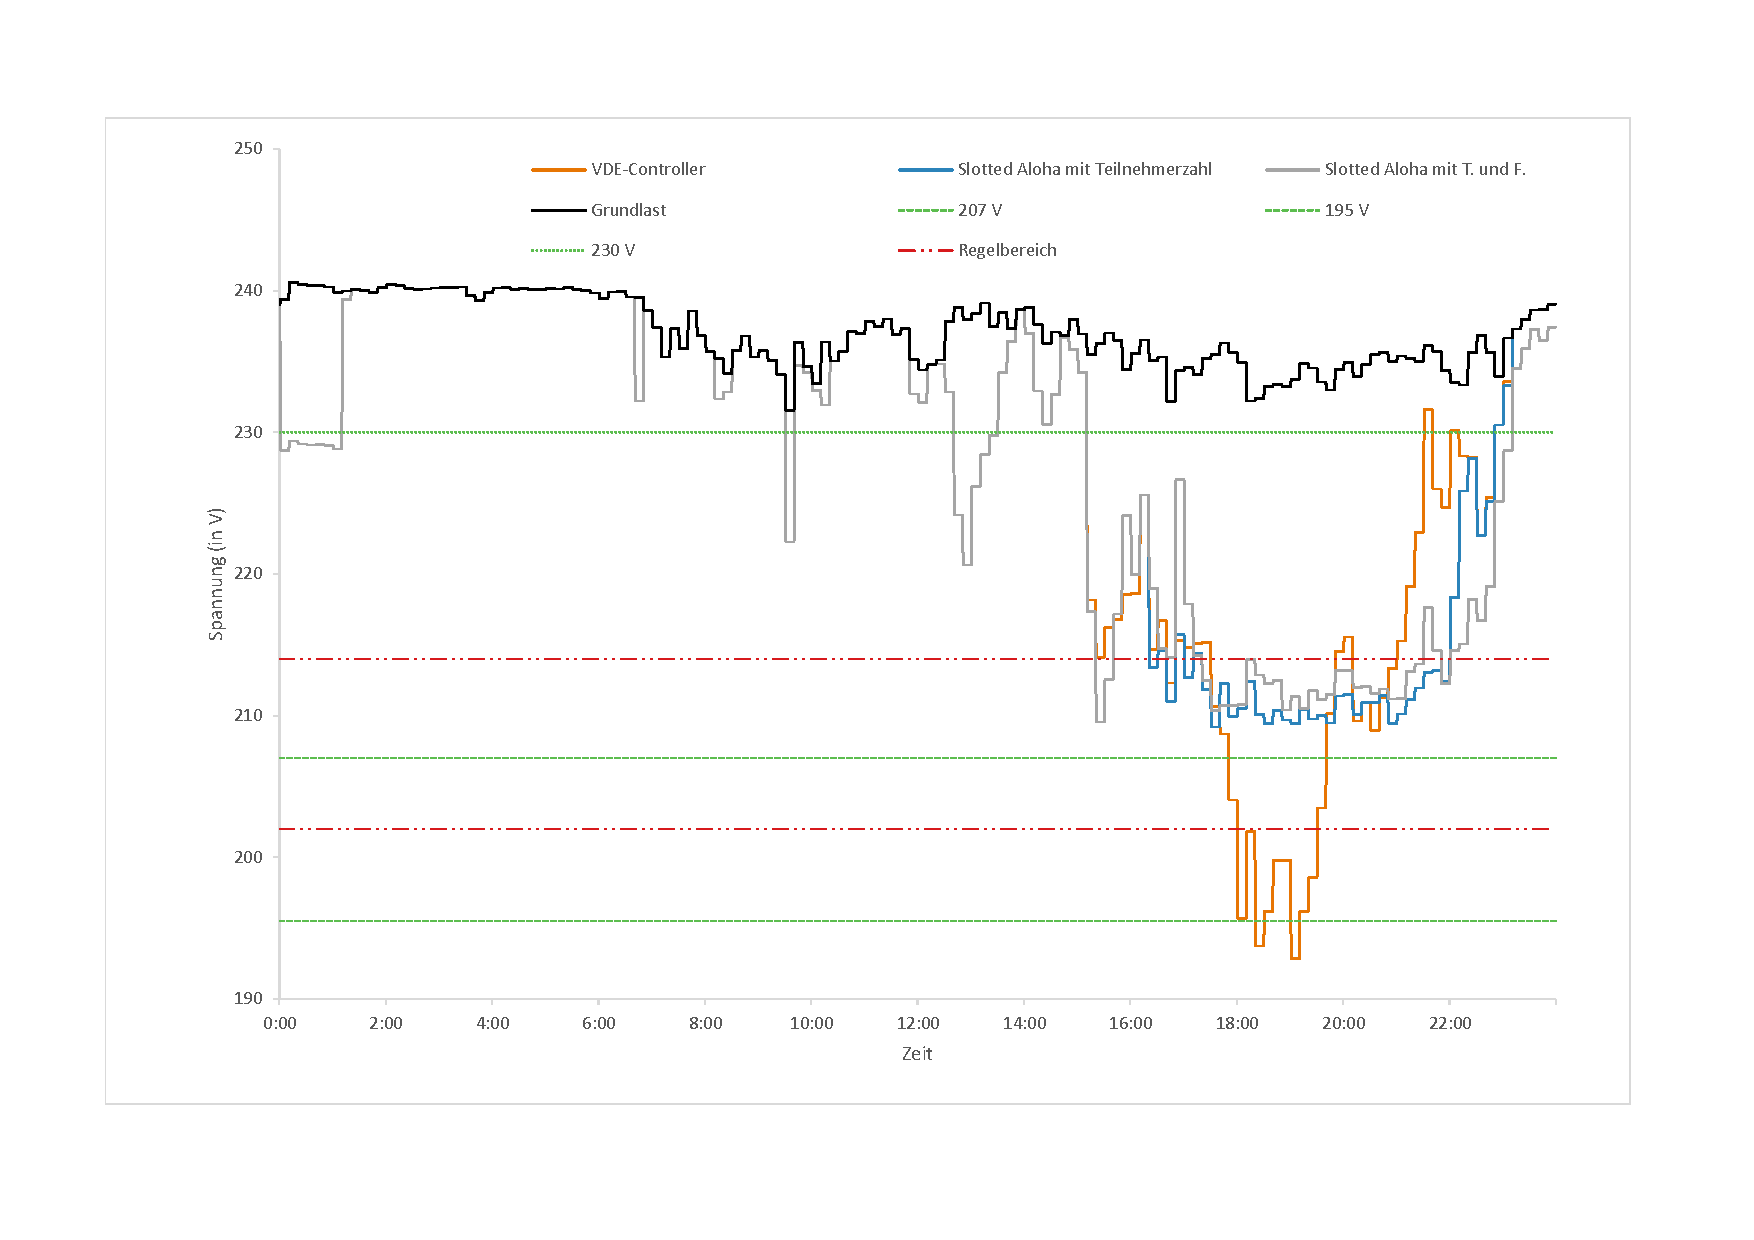
\includegraphics[scale=0.5]{img/ohneTrafo/Spannung3.pdf}
		\caption{10 Minuten Mittelwerte der Spannung über den Verlauf eines Tages}
		\label{Abb_oT_Spannung}
	\end{subfigure}
\end{figure}
In Abbildung \ref{Abb_oT_TrafoLast} wird der Leistungsbezug am Transformator, welcher von jeder der drei Methodiken verursacht wurde, abgebildet. Der Regelbereich ist hier zwar angetragen, jedoch verfügt keine der hier dargestellten Techniken über den entsprechenden Controller. Anders als bei den Einzelanalysen wird hier auf das abbilden der Standardabweichung verzichtet, um eine bessere Übersichtlichkeit zu erhalten. An den Graphen wird der Effekt der Verwendung des Slotted Aloha Protokolls deutlich. Die Transformatorlast, wenn nur der VDE-Controller verwendet wird, schwankt stärker und erreicht höhere Werte als die beiden Varianten, welche das Slotted Aloha Protokoll verwenden. Die beiden Varianten, welche das Protokoll verwenden, weisen ähnliche Werte auf, beider Arten der Bestimmung der Wartezeiten zeigen hier, dass das Konzept funktioniert und zu einer Besserung der Werte beitragen kann. Diese Besserung stellt ein unabhängig von der Art der Bestimmung der Wartezeit. Das spätere Sinken der Last, wenn die Variante verwendet wurde, welche die Fahrzeugparameter mitbetrachtet, zeigt diese Die Ladevorgänge bei dieser Variante auf längere Zeit verteilt wurden, dies ist auch an dem gelegentlich niedrigeren werten bereits ablesbar.\\
Abbildung \ref{Abb_oT_Spannung} zeigt die minimalen 10 Minuten Mittelwerte aller Anschlusspunkte des Niederspannungsnetzes. Der angetragene Regelbereich kennzeichnet den Bereich, in dem der Spannungskontroller aktiv wird und den möglichen Lastbezug regelt. Auch in dieser Abbildung werden die jeweiligen Standardabweichungen zur besseren Übersichtlichkeit nicht dargestellt. Im Vergleich über die drei hier dargestellten Methodiken zeigt sich, wie bereits bei der Transformatorlast, dass der VDE-Kontroller ohne Slotted Aloha nicht in der Lage ist die Werte ausreichend zu kontrollieren. Die beiden Methodiken, welche das Slotted Aloha Protokoll mitverwenden, zeigen anhand ihrer Graphen, wie der Spannungskontroller seinen angedachten Zweck erfüllt. Die Werte fallen zwar auch in den Regelbereich ab, bleiben allerdings oberhalb der unteren Grenze des Regelbereiches. Der Verlauf der beiden Graphen, währenddessen sie im Regelbereich liegen, zeigt einen ähnlichen Verlauf ohne zu große Schwankungen. Auch bei der Spannung erholen sich die Werte, bei der Variante, welche nur die Teilnehmeranzahl verwendet, schneller als bei der anderen Variante, welche das Slotted Aloha Protokoll mitverwendet. Allerdings ist am Verlauf des Graphen auch erkennbar, dass die Werte, wenn die Variante mit Teilnehmeranzahl und Fahrzeugparameter verwendet wird im Regelbereich des Kontrollers noch am höchsten sind und nur die Rückkehr zur Grundlast etwas länger dauert.
\begin{figure}
	\begin{subfigure}{\linewidth}
		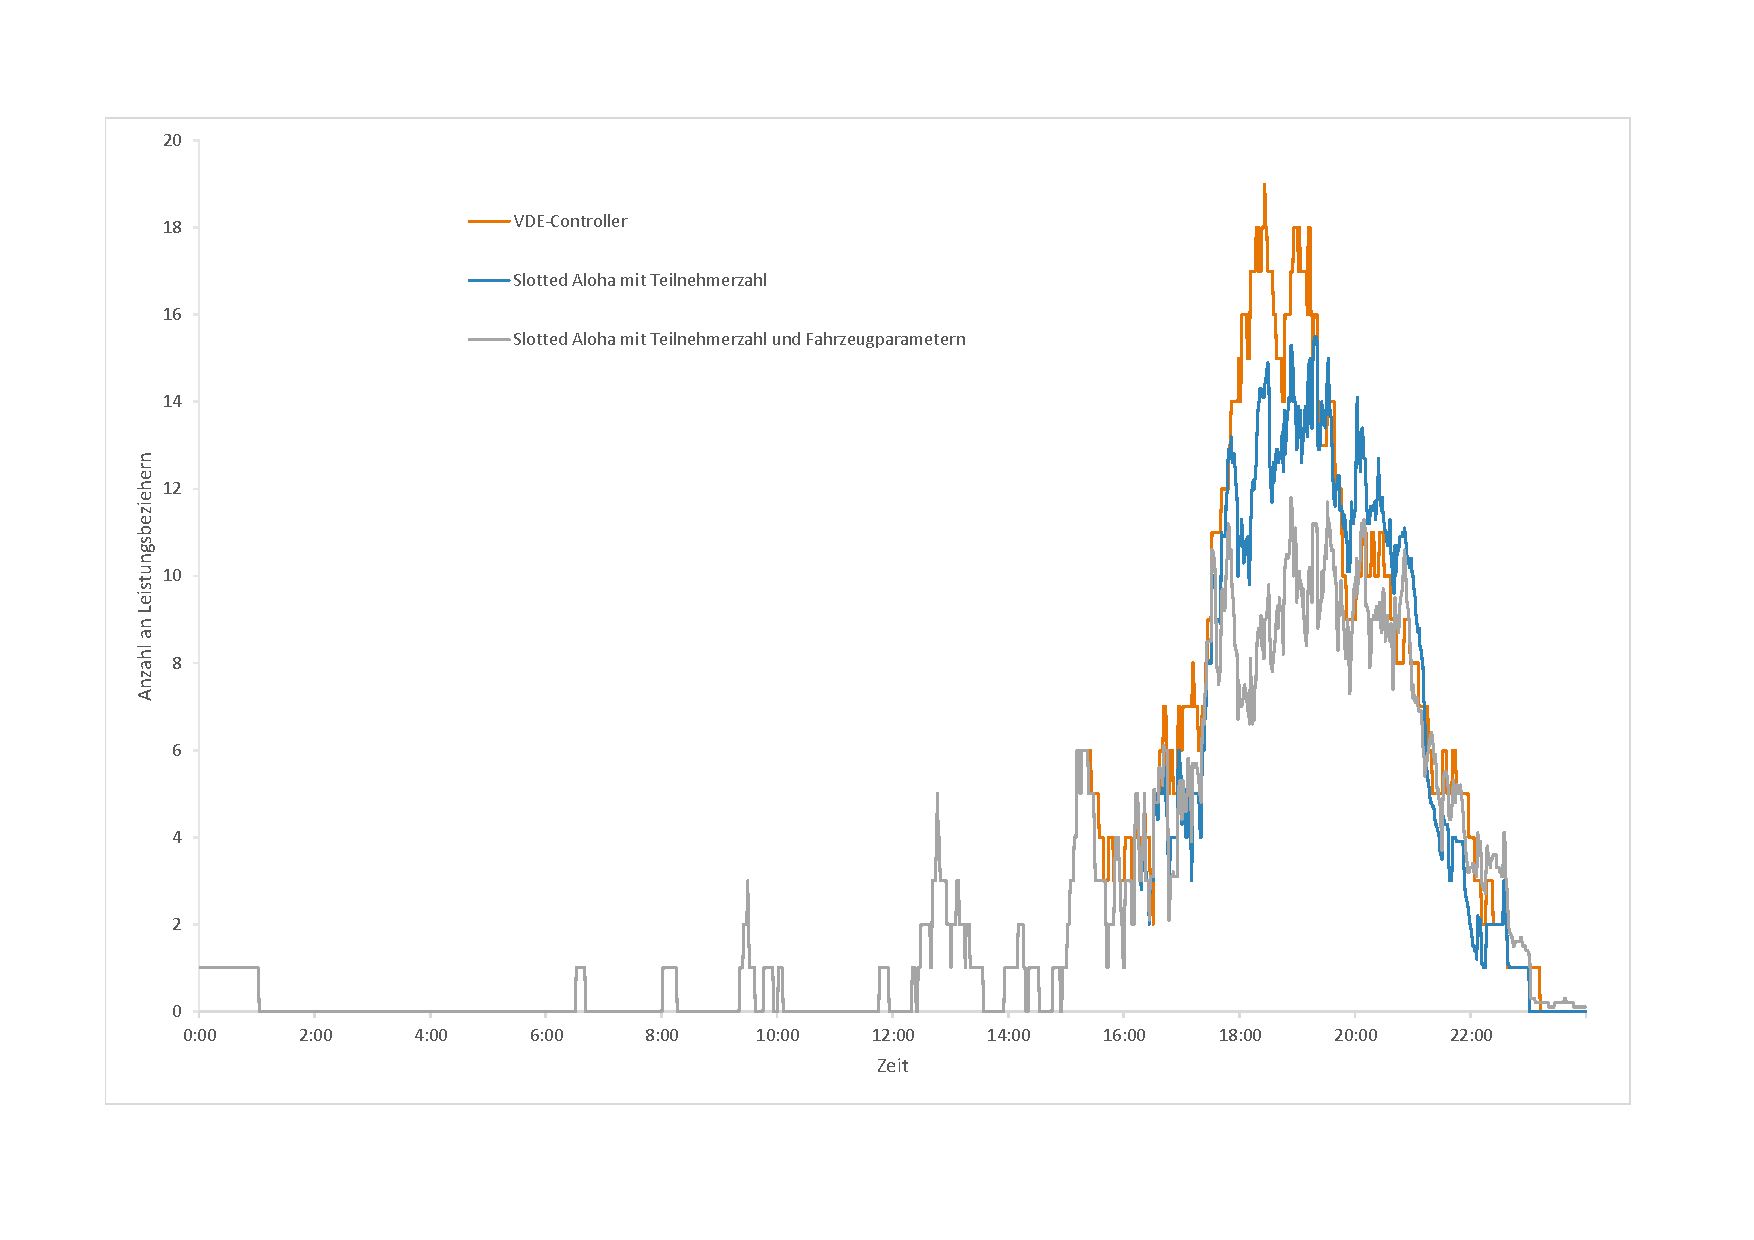
\includegraphics[scale=0.5]{img/ohneTrafo/Teilnehmer2.pdf}
        \subcaption{Anzahl der ladenden Teilnehmer über den Verlauf eines Tages}
        \label{ABB_oT_Teil1}
	\end{subfigure}
	\begin{subfigure}{\linewidth}
		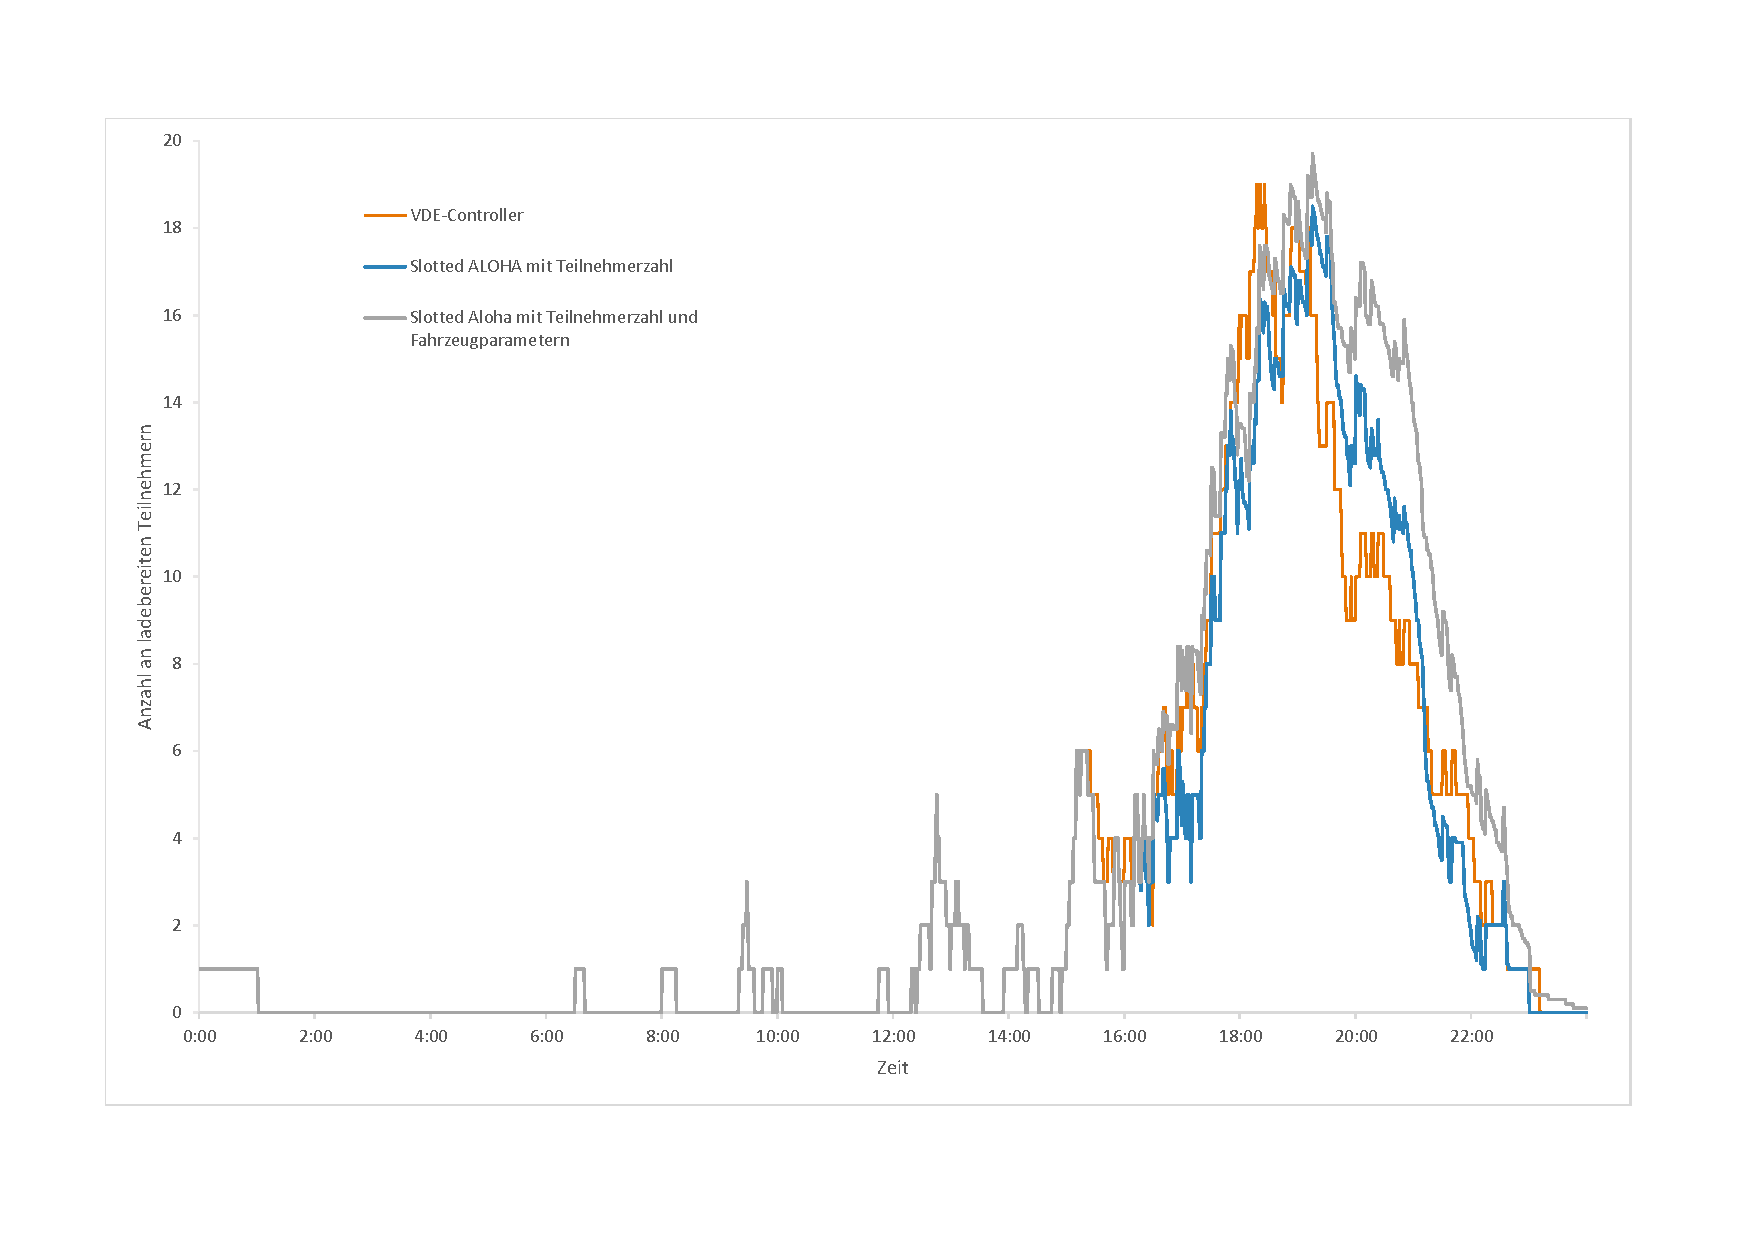
\includegraphics[scale=0.5]{img/ohneTrafo/Teilnehmer3.pdf}
        \subcaption{Anzahl der ladendbereiten Teilnehmer über den Verlauf eines Tages}
        \label{ABB_oT_teil2}
	\end{subfigure}
\end{figure}
In Abbildung \ref{ABB_oT_Teil1} sind die jeweiligen Anzahlen der ladenden Teilnehmer und in Abbildung \ref{ABB_oT_teil2} die jeweiligen Anzahlen der ladebereiten Teilnehmer dargestellt. An der Zahl der Teilnehmer ist erkennbar, dass die über alle drei Methoden hinweg die zahl der ladebereiten Teilnehmer immer relativ ähnlich ist, während sich bei der Anzahl der ladenden Teilnehmer teils sichtbare Unterschiede einstellen. Bei der Methode, wo sowohl Teilnehmerzahl als auch Fahrzeugparameter verwendet werden, laden meist weniger Teilnehmer gleichzeitig, dafür gibt es über einen längeren Zeitraum mehr lade Bereite Teilnehmer. Bei der Anzahl der ladenden Teilnehmer zeigt sich der Unterschied in der Bestimmung der Ladezeiten, durch die Möglichkeit längere Wartezeit zu bestimmen, da durch die Verwendung der Fahrzeugparameter die Ergebnismenge nicht mehr durch die Anzahl an Ladebereiten Teilnehmern beschränkt ist. Die hier sichtbare unterschiedliche Verteilung der ladenden Teilnehmer zeigte sich bereits bei der Transformatorlast und den Spannungswerten.
Beim Vergleich über die Transformatorlast, den Spannungsverlauf und die Teilnehmerzahlen zeigt sich, dass die beiden Varianten, die das Aloha Protokoll mitverwenden dem VDE-Controller ohne Erweiterung überlegen sind. Die Transformatorlasten sind deutlich kontrollierter und die Spannungswerte liegen höher. Diese Muster setzt sich bei der Betrachtung der Einhaltung der Norm DIN EN 50160 fort, von den drei betrachteten Methoden ist lediglich der VDE-Controller nicht in der Lage diese Norm zu erfüllen.
Für alle drei Methoden wurde die Anzahl an Situation bestimmt, in denen eine Spannungskollision auftreten könnte.
\begin{table}[]
\centering
\begin{tabular}{l|l|l|l|}
\cline{2-4}
                                                                                       & Variante       &                                                                             &                                                                        \\ \hline
\multicolumn{1}{|l|}{}                                                                 & VDE-Kontroller & \begin{tabular}[c]{@{}l@{}}Slotted ALOHA \\ mit Teilnehmerzahl\end{tabular} & \begin{tabular}[c]{@{}l@{}}Slotted Aloha \\ mit T. und F.\end{tabular} \\ \hline
\multicolumn{1}{|l|}{\begin{tabular}[c]{@{}l@{}}mögliche \\ Situationen\end{tabular}}  & 1535           & 668,7 (+-)                                                                 & 392,6 (+-)                                                            \\ \hline
\multicolumn{1}{|l|}{\begin{tabular}[c]{@{}l@{}}Anzahl an \\ Wartezeiten\end{tabular}} & 0              & 553,9 (+-)                                                                   & 246,9 (+-)                                                            \\ \hline
\end{tabular}
\caption{Anzahl der möglichen und tatsächlich aufgetreten Kollisionen}
\label{tab:my-table3}
\end{table}

Anhand Tabelle \ref{tab:my-table3} zeigt sich erneut die Verbesserung die erzielt wird, wird eine Variante verwendet, welche mit Teilen des Netzwerkprotokolls erweitert wurde. Je nach verwendeter Variante treten nur noch halb bzw. ein Viertel so viele Situationen ein, wo eine Spannungskollision auftreten könnte. Jedoch zeigt sich auch beim Vergleich der beiden Varianten, welche das Protokoll mitverwenden, wie sich die Arten der Wartezeitbestimmung unterscheiden, da auch hier, wenn Teilnehmerzahl und Fahrzeugparameter verwendet werden, die Anzahl an Situationen um mehr als ein Drittel reduziert werden kann. Mit der Anzahl der möglichen Kollisionen sinkt auch die Zahl der aufgetretenen Kollisionen. Beim Verhältnis zwischen möglichen und tatsächlich aufgetretenen Kollisionen, zeigt sich, dass wenn die Fahrzeugparameter mitberücksichtigt werden, in weniger Situationen wo eine Kollision auftreten kann auch eine Kollision auftritt. Wird nur die Teilnehmerzahl verwendet wird in etwa 80 \% der möglichen Situationen auch eine Wartezeit bestimmt, werden nun zusätzlich die Fahrzeugparameter berücksichtigt sinkt dieser Wert auf etwa 60 \% ab. 
\begin{figure}
	\begin{subfigure}{0.49\linewidth}
		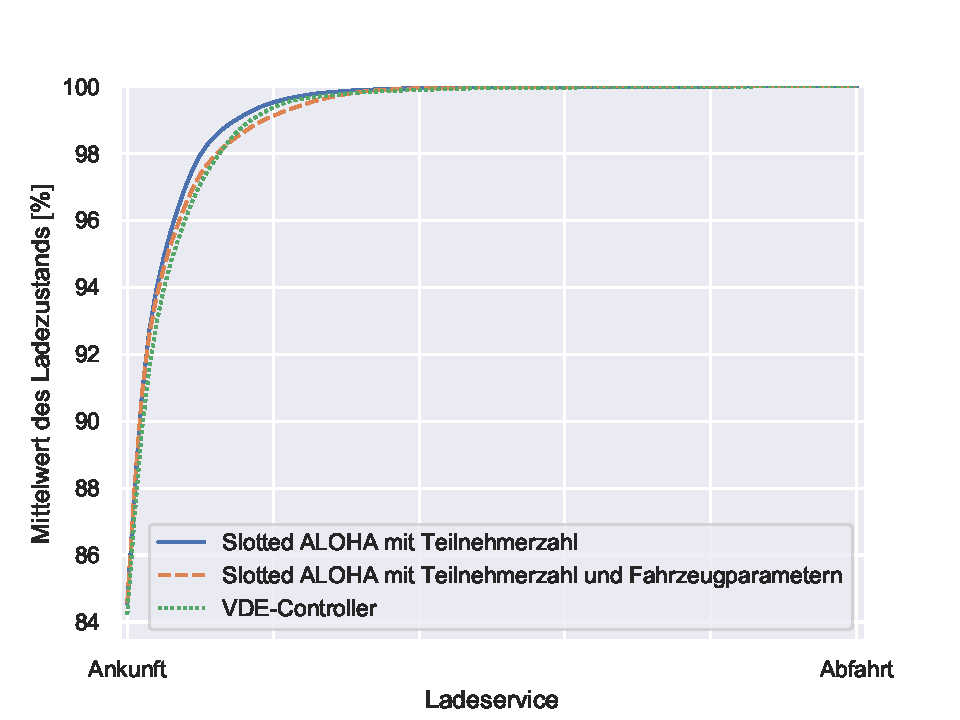
\includegraphics[width=\linewidth]{img/ohneTrafo/SlottedAloha_participants_VDE_tau_15_soc_mean.pdf}
        \subcaption{Durchschnittlicher Ladezustand aller Elektrofahrzeuges über den Verlauf eines Ladeservices}
        \label{ABB_ot_SocMEAN}
	\end{subfigure}
	\begin{subfigure}{0.49\linewidth}
		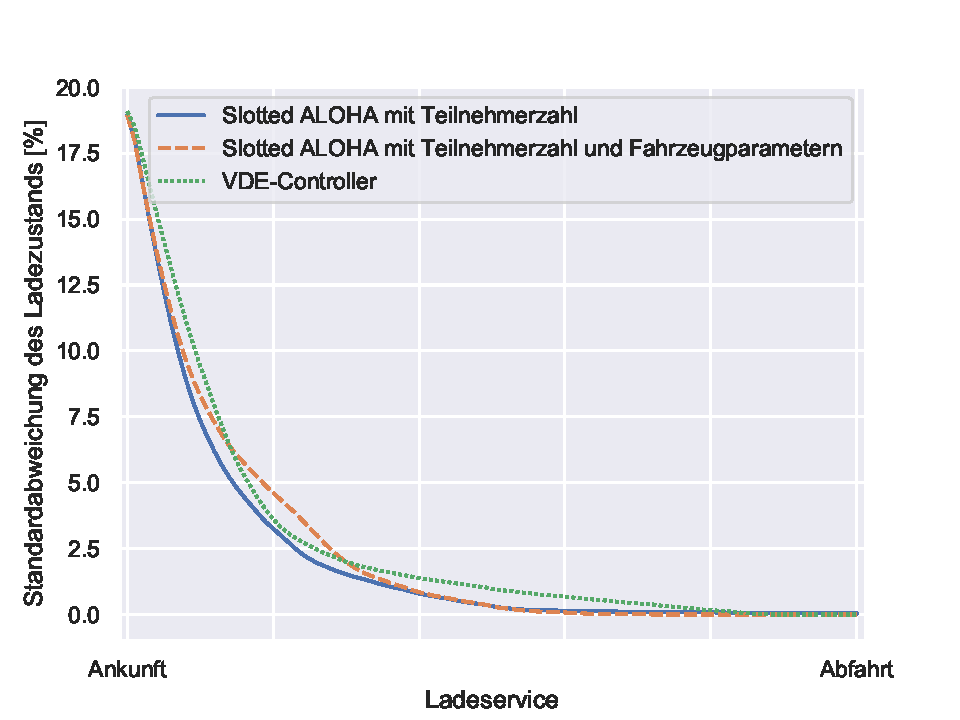
\includegraphics[width=\linewidth]{img/ohneTrafo/SlottedAloha_participants_VDE_tau_15_soc_std.pdf}
        \subcaption{Durschschnittliche Standardabweichung des Ladezustandes aller Elektrofahrzeuges über den Verlauf eines Ladeservices}
        \label{ABB_oT_SocSTD}
	\end{subfigure}
\end{figure}

In Abbildung \ref{ABB_ot_SocMEAN} sind die jeweiligen mittleren Ladestände aller Fahrzeugen über den Verlauf der Ladeservice hinweg dargestellt, Abbildung \ref{ABB_oT_SocSTD} zeigt die zugehörige Standardabweichung. Abbildung \ref{ABB_ot_SocMEAN} zeigt einen ähnlichen Verlauf der Kurven für alle drei Varianten, wird allerdings zusätzlich die dazugehörige Standardabweichung betrachtet zeigen sich Unterschiede. Diese Unterschiede weisen erneut auf das bekannte Verhältnis zwischen den Varianten hin. Sichtbar wird auch die Ähnlichkeit der beiden Varianten, welche Wartezeiten verwenden.
\begin{figure}[htb]
\centering
	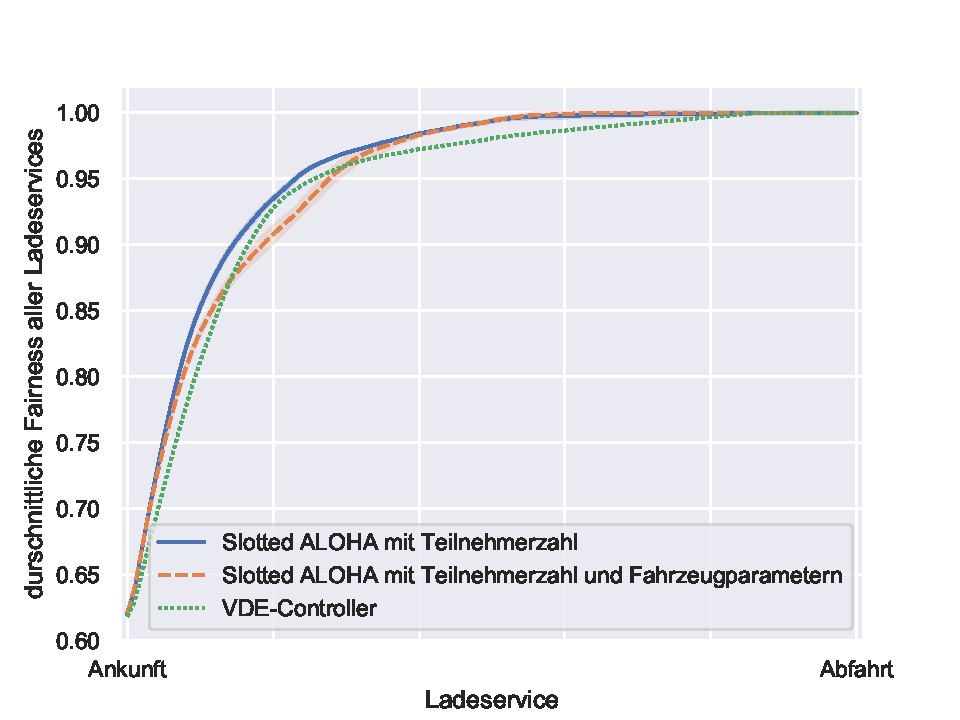
\includegraphics[scale=0.6]{img/ohneTrafo/SlottedAloha_participants_VDE_tau_15_qoe.pdf}
	\caption{Durchschnittlicher Qualitätserfahrung aller Elektrofahrzeuges über den Verlauf eines Ladeservices}
	\label{Abb_oT_Fairness}
\end{figure}
Abbildung \ref{Abb_oT_Fairness} zeigt die mittlere Fairness aller Fahrzeuge über den Verlauf der Ladeservice hinweg mit der zugehörigen Standardabweichung für alle drei betrachteten Varianten. Der Verlauf der drei Kurven weist auch hier wieder große Ähnlichkeiten auf. Allerdings erreichen die beiden Varianten, welche Teile des Aloha Netzwerkprotokolls verwenden, den maximalen Wert deutlich früher als der VDE-Kontroller. Die beiden Varianten mit dem Netzwerkprotokoll erreichen den maximal Wert nahezu gleichzeitig, im Verlauf der Graphen zeigen sich dennoch Unterschiede. Der teils langsamere Anstieg kann auf die bessere Verteilung der Ladevorgänge über die Zeit zurückgeführt werden. Diese bessere Verteilung hat sich bei der Betrachtung bisher als positive Eigenschaft herausgestellt und mindert auch hier das eigentlich erreichte Ergebnis nicht.
Nach Betrachtung der Eigenschaften über alle drei Varianten hat sich herausgestellt, dass die Varianten, welche teile des Aloha Protokolls verwenden, bessere Ergebnisse geliefert haben als der VDE-Kontroller ohne Erweiterung. Aus dem Vergleich ging des Weiteren hervor, dass die Variante, welche die Teilnehmerzahl und die Fahrzeugparameter verwendet, das optimalste Ergebnis liefert. Diese Variante sorgt für höhere Spannungen, niedrige Transformatorlasten, es kommen am wenigsten Situationen vor, in denen eine Spannungskollision auftreten könnte und all das wird erreicht während zudem der Zeitpunkt, an dem maximal mögliche Fairness zwischen den Teilnehmern erreicht wird, nach vorne verlegt wird.

\subsection{Vergleich der Varianten mit Transformatorkontroller}
Die Ergebnisse der drei Varianten, welche den Transformatorkontroller verwenden, wurden bereits jeweils für sich analysiert, nun folgt der Vergleich über die drei Varianten hinweg. Wie bereits bei der Analyse des VDE-Controllers mit dem Transformatorkontroller erwähnt wurde, musste bei dieser Variante der verwendete Lag-Filter geändert werden, um einen erfolgreichen und vollständigen Durchlauf zu erhaltenen. Diese Änderung beeinflusst auch das Ergebnis dieses Vergleichs, da sie nur bei einer Methodik notwendig war und die anderen beiden Varianten, einen anderen Lag-Filter verwenden.\\
Die drei Varianten werden dennoch anhand der Transformatorlast, den 10 Minuten Mittelwerten der Spannung, der Teilnehmerzahl verglichen. Ebenso betrachtet wird die Qualität der Ladevorgänge und die Fairness wird über alle drei Methodiken. Wie bei den einzelnen Analysen wird auch hier, bei der Transformatorlast, den Spannungswerten und der Teilnehmerzahl, wieder ein Werktag aus dem simulierten Zeitraum von einer Woche dargestellt.\\
\begin{figure}
	\begin{subfigure}{\linewidth}
		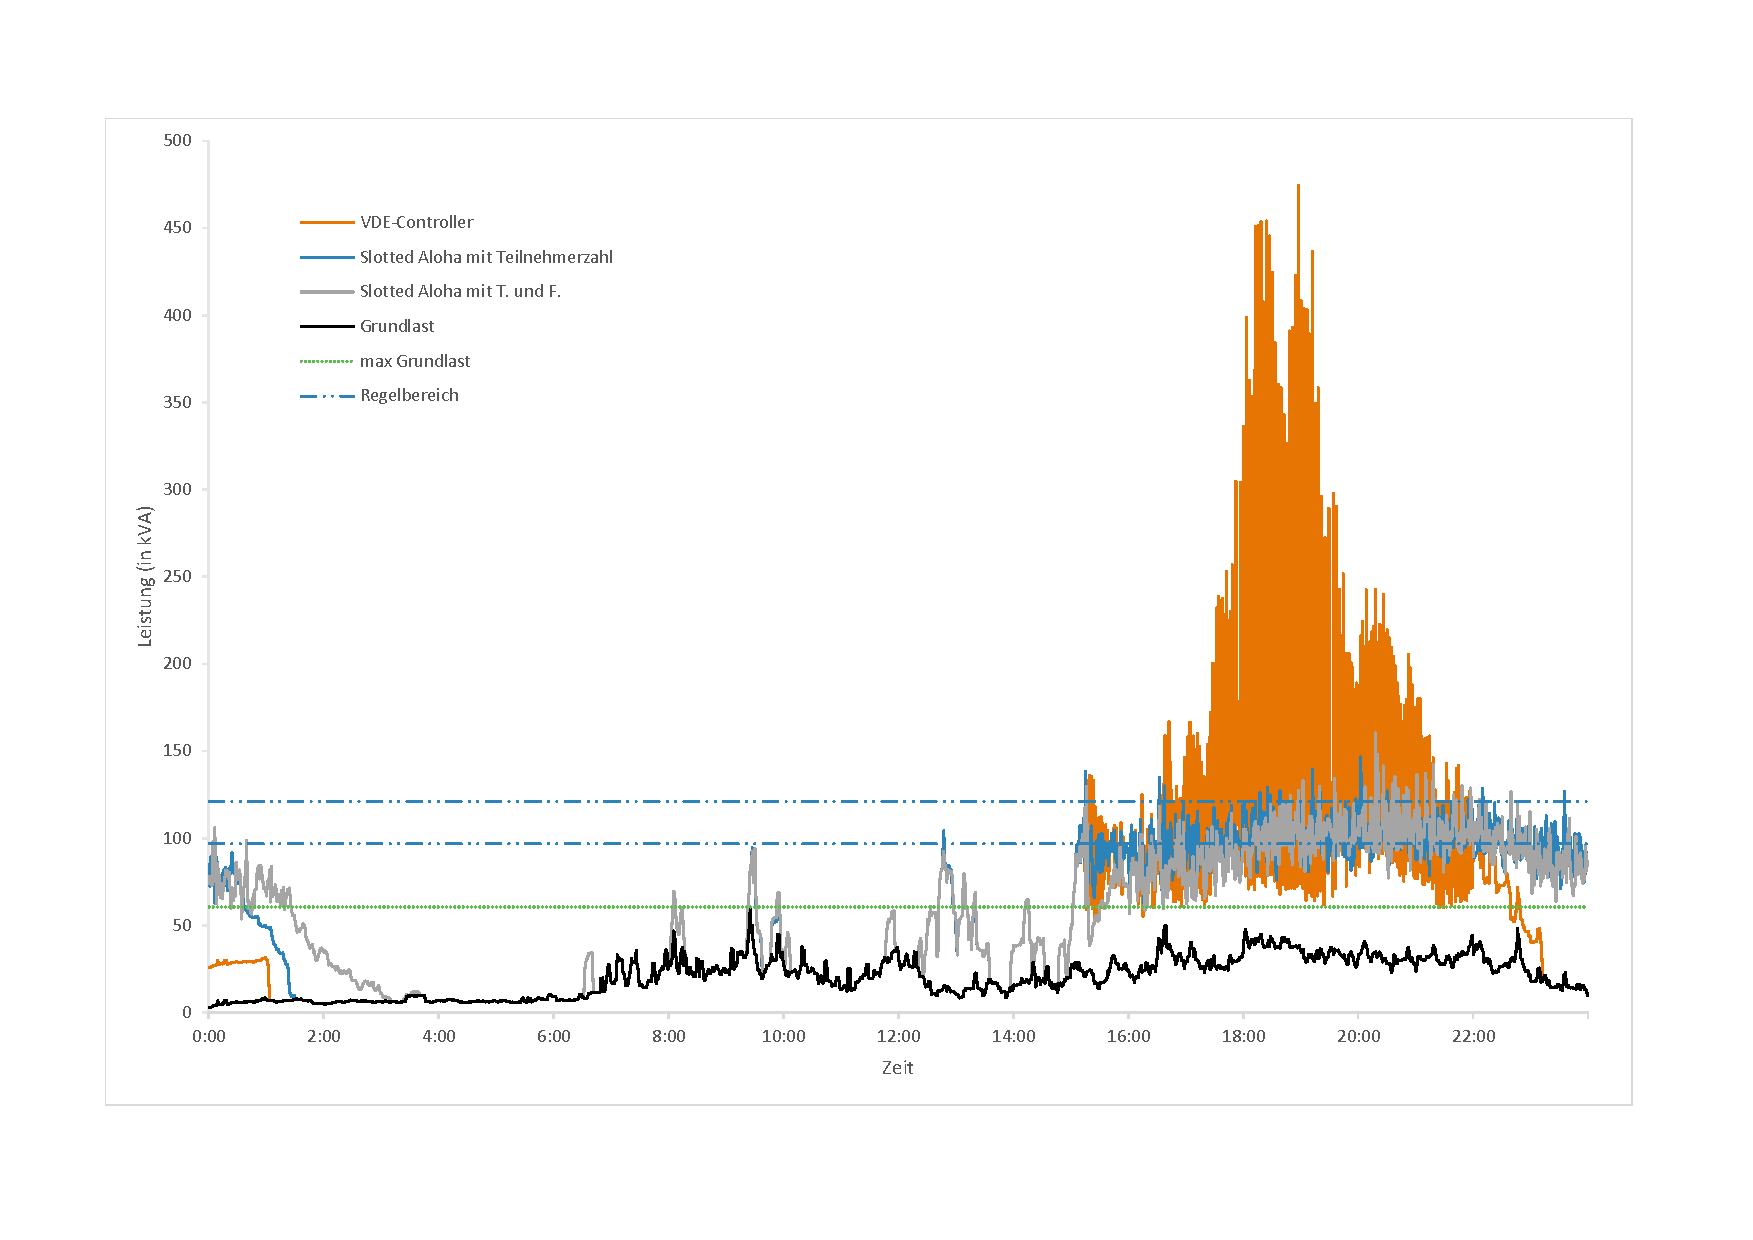
\includegraphics[scale=0.5]{img/mitTrafo/Trafolast.pdf}
        \subcaption{Transformatorlast über den Verlauf eines Tages}
        \label{ABB_mT_Trafo}
	\end{subfigure}
	\begin{subfigure}{\linewidth}
		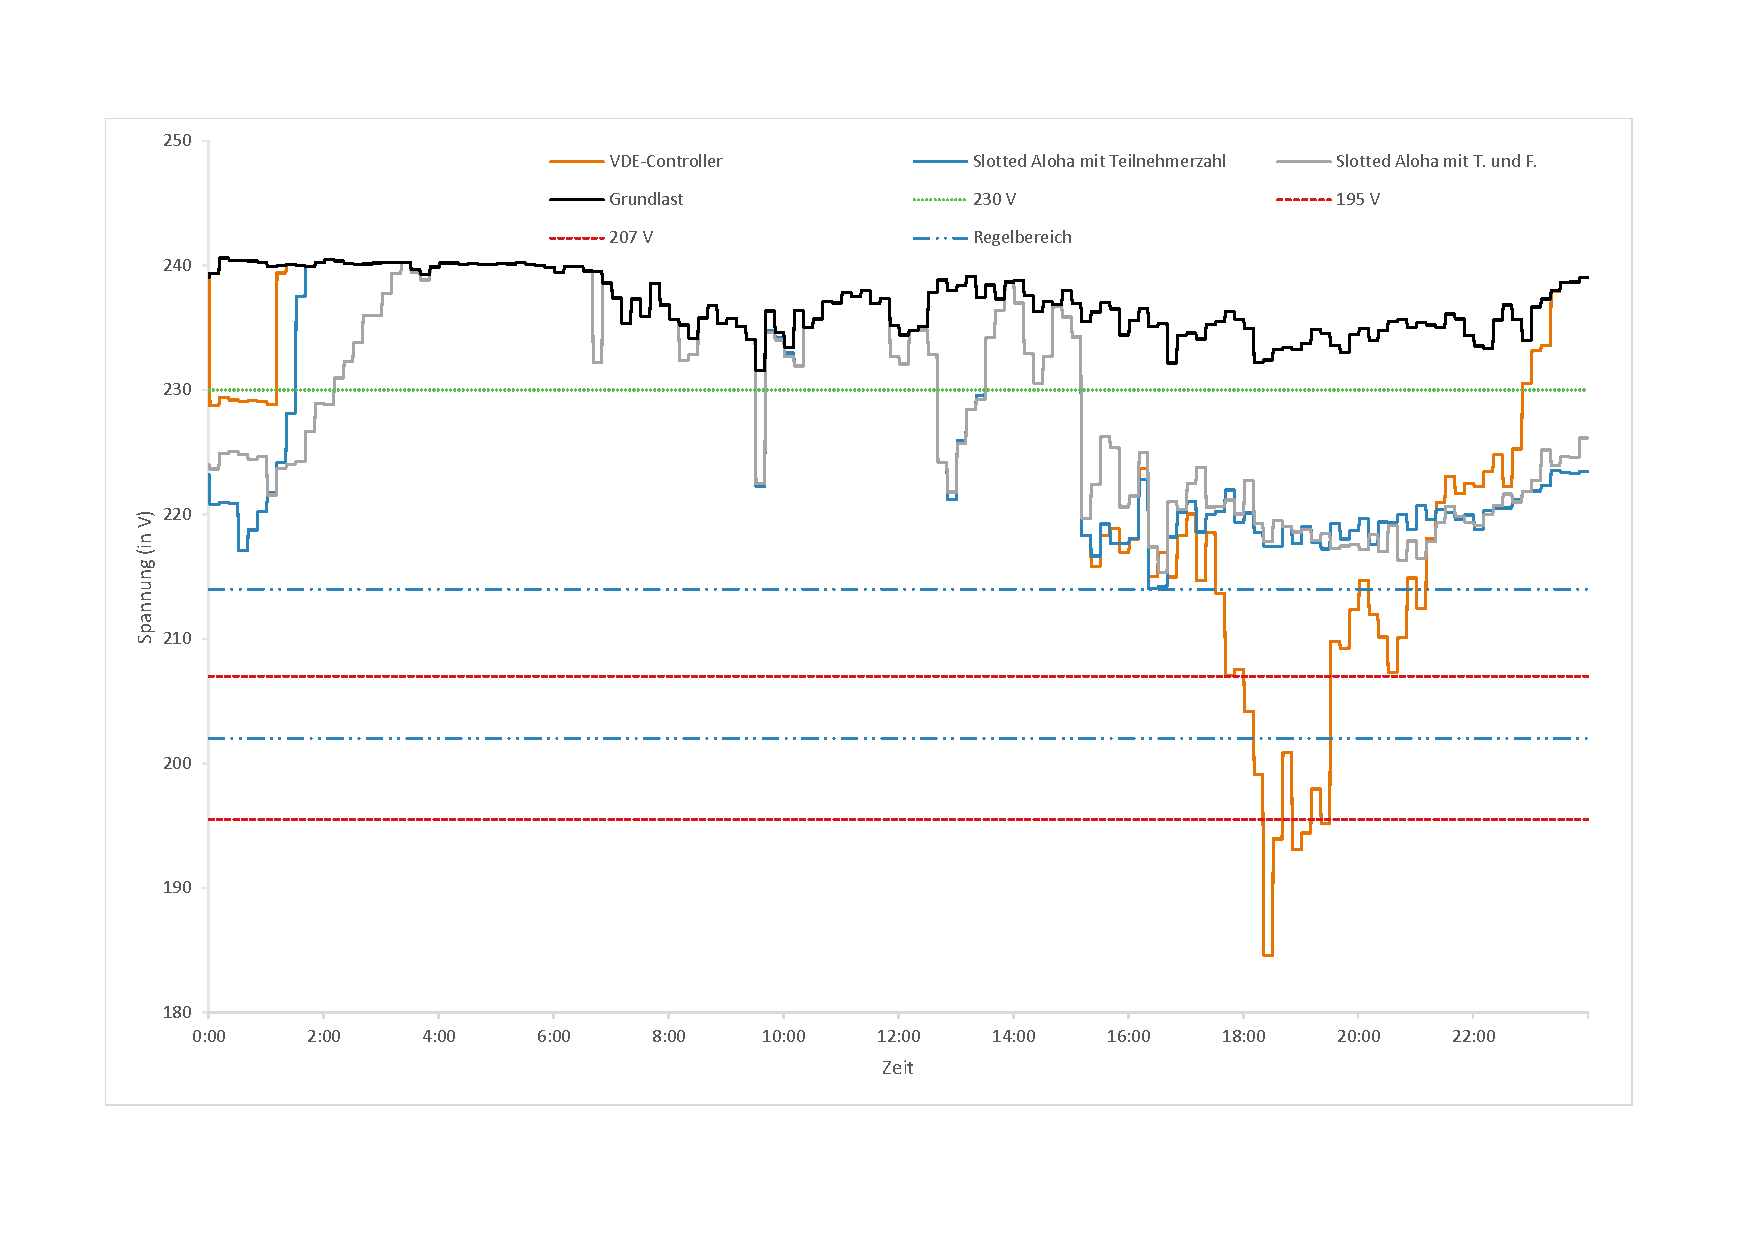
\includegraphics[scale=0.5]{img/mitTrafo/Spannung.pdf}
        \subcaption{10 Minuten Mittelwerte der Spannung über den Verlauf eines Tages}
        \label{ABB_mT_Spannung}
	\end{subfigure}
\end{figure}
In Abbildung \ref{ABB_mT_Trafo} sind die mittleren Transformatorlasten der drei verwendeten Methoden angetragen. Der nach unten und oben abgegrenzte Regelbereich markiert den Arbeitsbereich des Transformatorkontrollers. Einzelne Spitzen über den Regelbereich hinaus, lassen sich aufgrund der dezentralen Verwendung kaum verhindern, da sich die einzelnen Teilnehmer nicht mit anderen abstimmen. Am Verlauf der Kurven erkennt man dasselbe Muster, welche sich bereits bei der Analyse aller drei Varianten ohne Transformatorkontroller gezeigt hat. Die Variante mit nur dem VDE-Controller oszilliert sehr stark und liefert die höchsten Werte aller drei Varianten. Die beiden Varianten, welche mit Teilen des Aloha Netzwerkprotokolls erweitert wurden, liefern sehr ähnliche Werte. Jedoch zeigt sich erneut, dass wenn die Fahrzeugparameter mit berücksichtigt werden, die Last zwar länger braucht um wieder auf das Niveau der Grundlast abzusinken, allerdings sind die werte auch etwas niedriger als, wenn nur die Teilnehmerzahl verwendet wird.\\
Abbildung \ref{ABB_mT_Spannung} zeigt die Mittelwerte von 10 Minuten Mittelwerten der Spannung, auf die Abbildung der dazugehörigen Standardabweichung wurde für eine bessere Übersichtlichkeit verzichtet. Hier wiederholt sich erneut das bereits festgestellte Muster. Der VDE-Controller ohne Erweiterungen liefert das schlechteste Ergebnis, während sich die Ergebnisse der beiden erweiterten Varianten sehr ähnlich sind. Ein merklicher Unterschied zwischen den beiden erweiterten Varianten lässt sich hier nur zum Beginn des betrachteten Zeitraumes feststellen, wo die Variante, welche die Teilnehmerzahl und die Fahrzeugparameter verwendet, zunächst höhere Werte aufweist, die Rückkehr auf das Niveau der Grundlast allerdings länger dauert.\\
\begin{figure}
	\begin{subfigure}{\linewidth}
		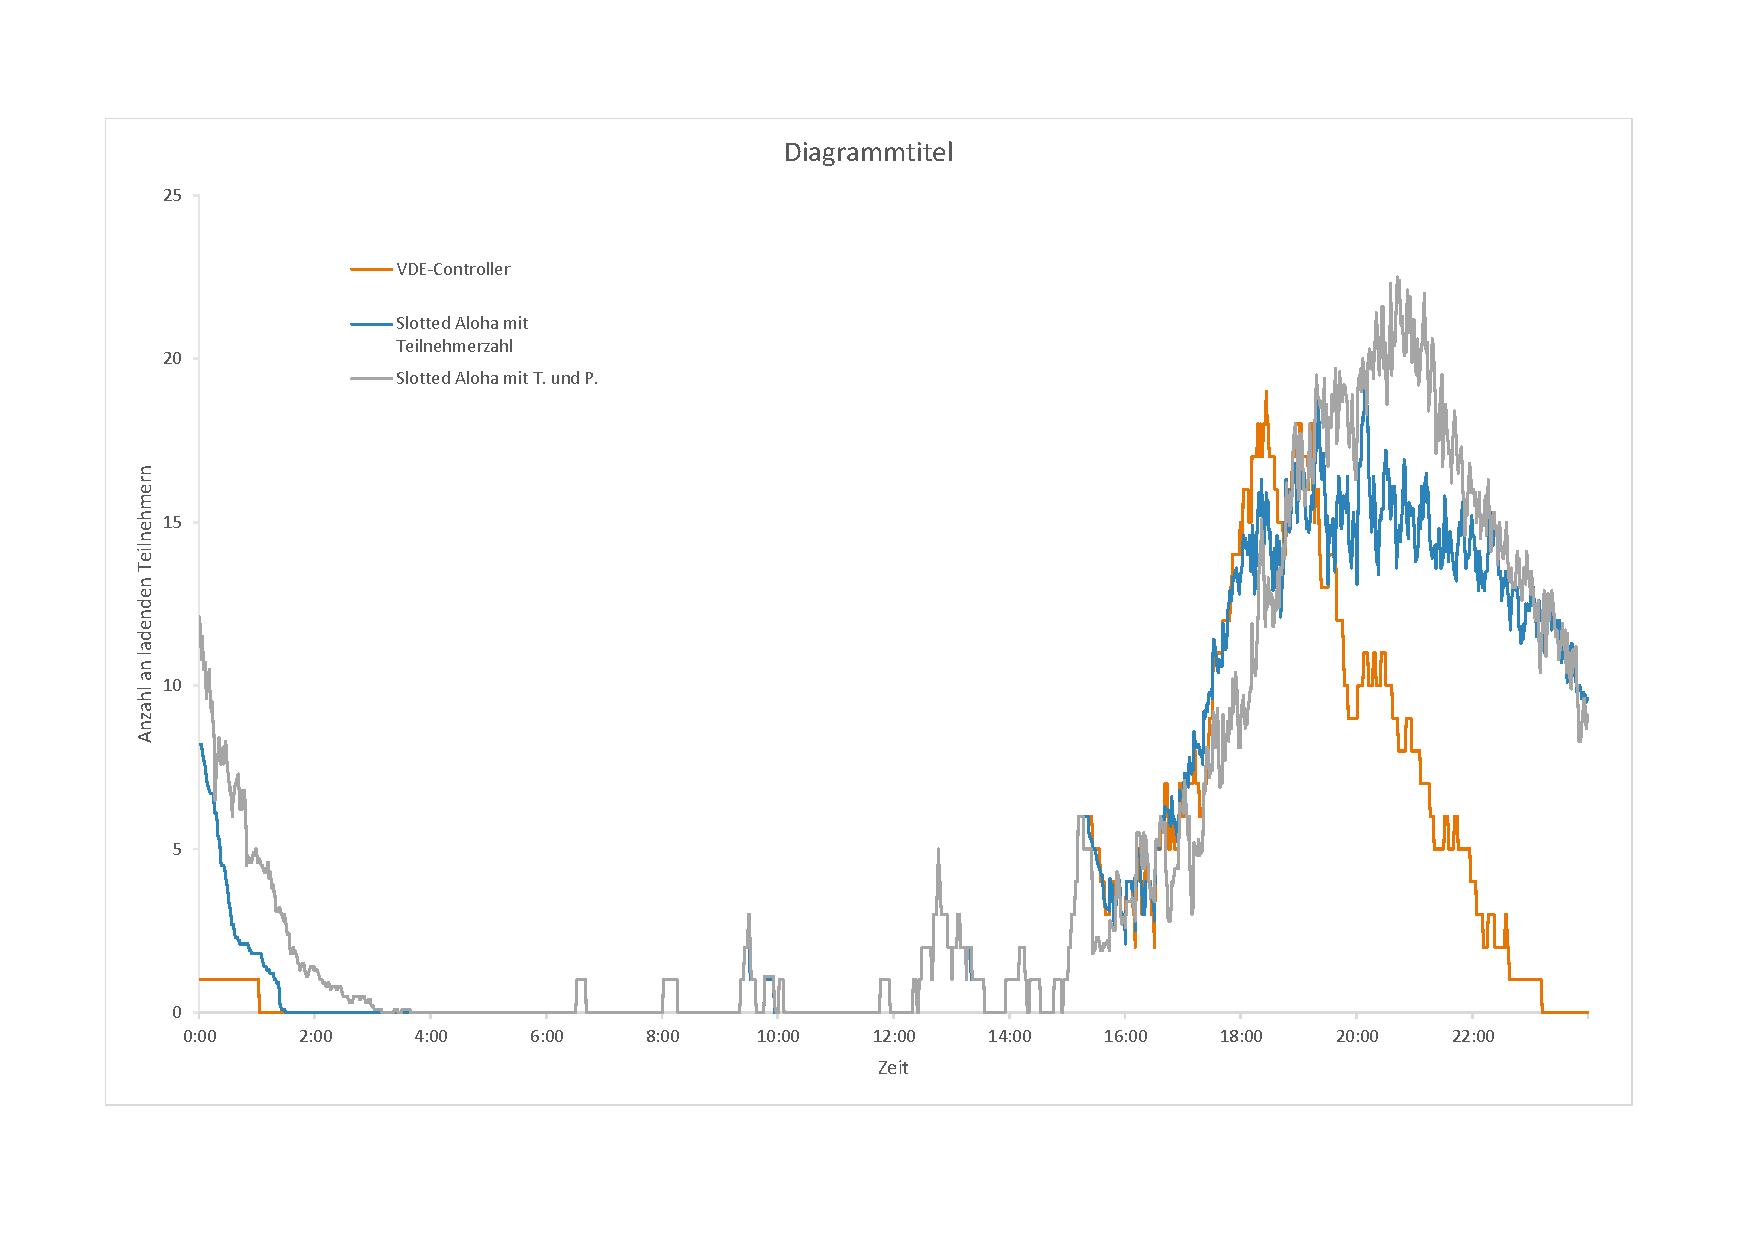
\includegraphics[scale=0.5]{img/mitTrafo/Teilnehmer1.pdf}
        \subcaption{Anzahl der ladenden Teilnehmer über den Verlauf eines Tages}
        \label{ABB_mT_Teil1}
	\end{subfigure}
	\begin{subfigure}{\linewidth}
		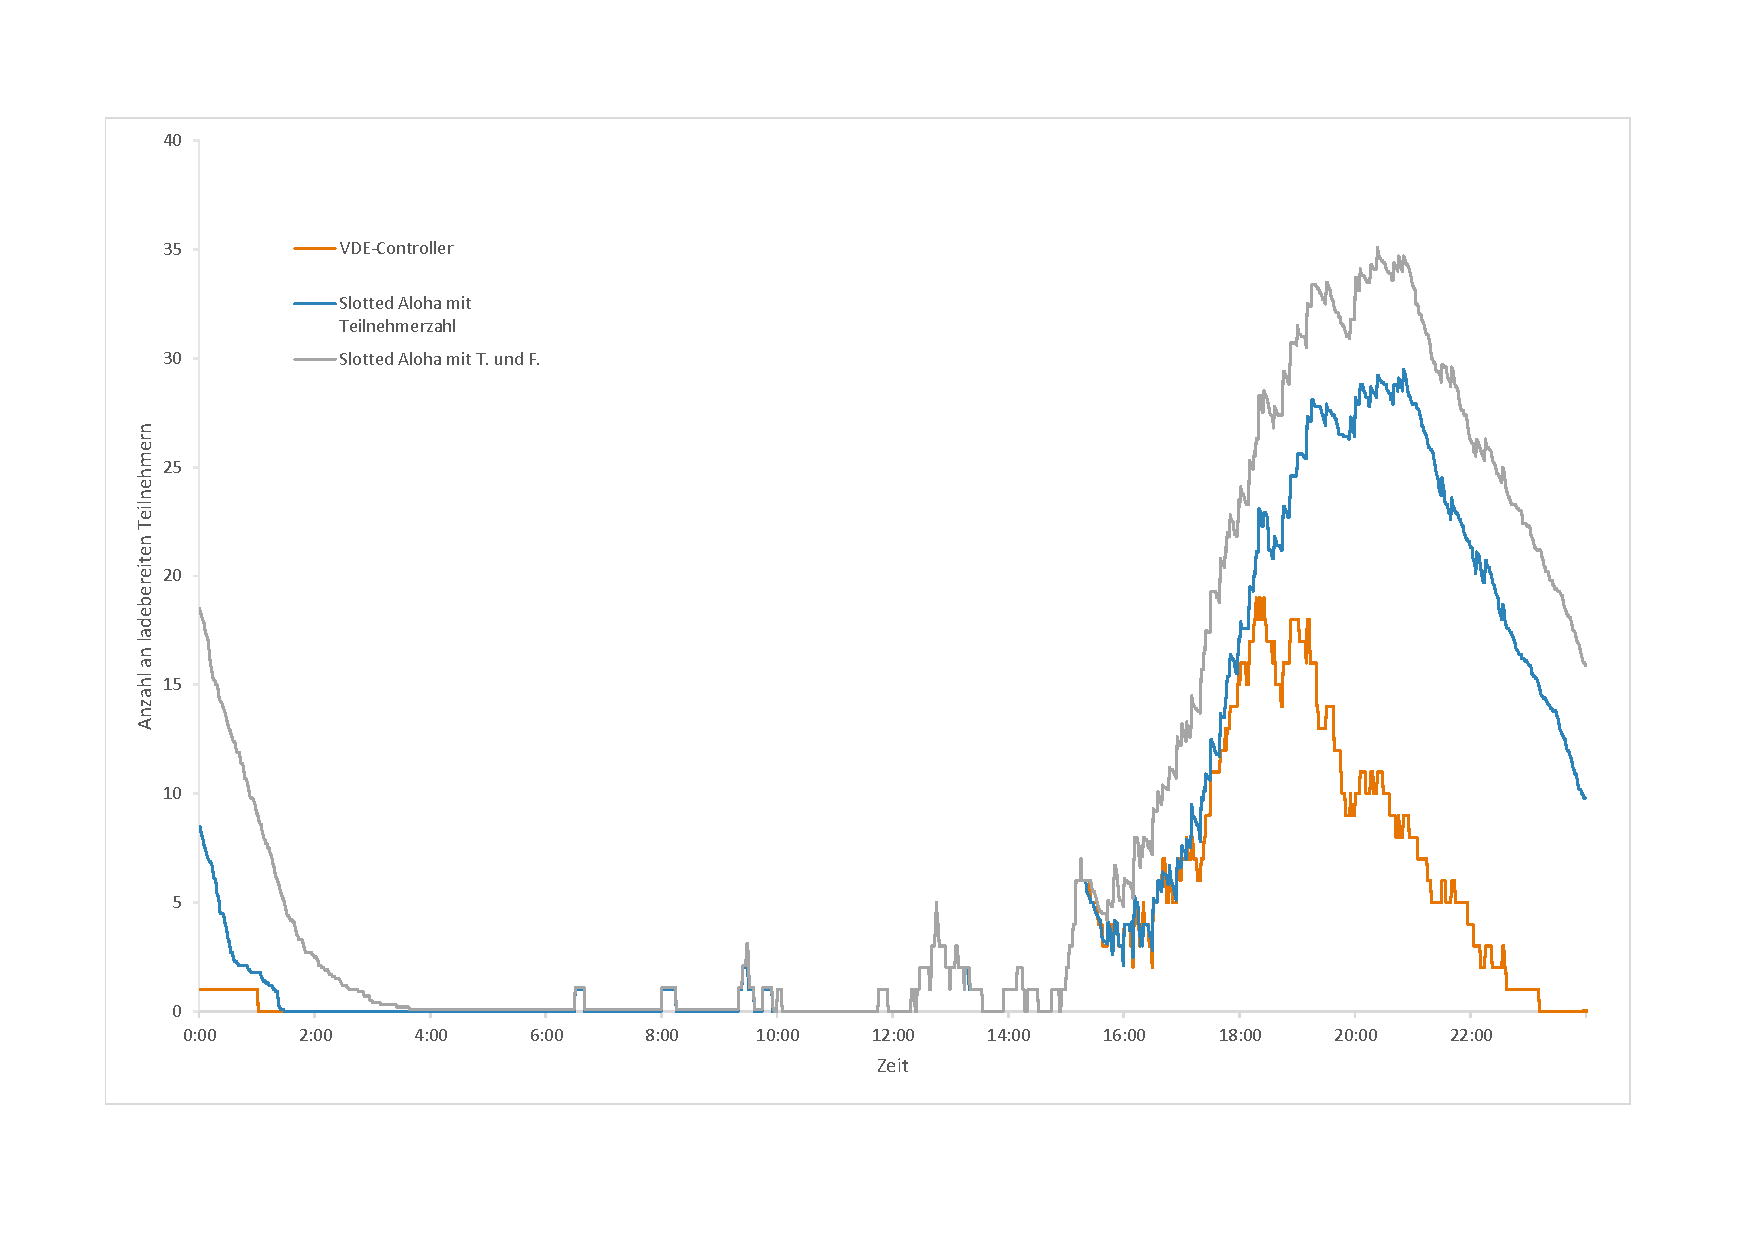
\includegraphics[scale=0.5]{img/mitTrafo/Teilnehmer3.pdf}
        \subcaption{Anzahl der ladendbereiten Teilnehmer über den Verlauf eines Tages}
        \label{ABB_mT_teil2}
	\end{subfigure}
\end{figure}
Abbildung \ref{ABB_mT_Teil1} zeigt die Anzahlen der ladebereiten Teilnehmer und Abbildung \ref{ABB_mT_teil2} zeigt die Anzahlen der ladenden Teilnehmer. Hier zeigen sich Unterschiede, welche bisher nicht ersichtlich waren. Durch die Limitierung der Ladeleistung durch den Transformatorkontroller, wird zwar die last am Transformator erfolgreich reduziert, allerdings baut sich auch die Menge an ladebereiten Fahrzeugen länger auf und langsamer wieder ab. Andererseits sind durch die reduzierte Leistungsaufnahme pro Teilnehmer mehr ladende Teilnehmer gleichzeitig möglich.
Beim Vergleich über die Transformatorlast, Die Spannungswerte und die Teilnehmerzahlen hinweg, zeigt sich dasselbe Ergebnis wie bereits beim Vergleich der Variante ohne den Transformatorkontroller. Der VDE-Controller ohne Erweiterungen liefert eine schlechtere Performanz ab als die beiden anderen Varianten, zusätzlich zu der Notwendigkeit der Überarbeitung der Technik um überhaupt auswertbare Ergebnisse zu liefern. Auch hier stellt sich die Variante, welche die Teilnehmerzahl und die Fahrzeugparameter verwendet, wieder als die Variante dar, welche die im aktuellen Vergleich besten Ergebnisse liefert. Der Abstand des VDE-Kontrollers zu den beiden Anderen setzt sich auch bei der Betrachtung der Norm DIN EN 50160 fort. Nur die beiden Varianten, welche Teile des Aloha Protokolls verwenden, sind in der Lage die Norm zu erfüllen.
Bei Betrachtung der Anzahl der möglichen Anzahl an Kollisionen zeigt sich zunächst ein anderes Bild als bisher.
\begin{table}[]
\centering
\begin{tabular}{l|l|l|l|}
\cline{2-4}
                                                                                       & Variante       &                                                                             &                                                                        \\ \hline
\multicolumn{1}{|l|}{}                                                                 & VDE-Kontroller & \begin{tabular}[c]{@{}l@{}}Slotted ALOHA \\ mit Teilnehmerzahl\end{tabular} & \begin{tabular}[c]{@{}l@{}}Slotted Aloha \\ mit T. und F.\end{tabular} \\ \hline
\multicolumn{1}{|l|}{\begin{tabular}[c]{@{}l@{}}mögliche \\ Situationen\end{tabular}}  & 5964           & 6589,3 (+-)                                                                 & 7077,0 (+-)                                                            \\ \hline
\multicolumn{1}{|l|}{\begin{tabular}[c]{@{}l@{}}Anzahl an \\ Wartezeiten\end{tabular}} & 0              & 3084 (+-)                                                                   & 2482,0 (+-)                                                            \\ \hline
\end{tabular}
\caption{Anzahl der möglichen und tatsächlich aufgetreten Kollisionen}
\label{tab:my-table4}
\end{table}

Tabelle \ref{tab:my-table4} zeigt die Anzahl der möglichen und die Anzahl der aufgetretenen Kollisionen. Anders als es zu erwarten war nach den bisherigen Ergebnissen, ist es bei der Variante mit den Fahrzeugparametern in mehr Situationen möglich, dass eine Kollision auftritt als in einer anderen Variante. Betrachtet man allerdings nun die Anzahl der tatsächlich aufgetretenen Kollisionen zeigt sich wieder das zu erwartende Muster. Trotz deutlicher mehr Situationen in denen eine Kollision auftreten könnte, treten bei der Variante mit den Fahrzeugparametern die wenigsten Kollisionen auf.
\begin{figure}
	\begin{subfigure}{0.49\linewidth}
		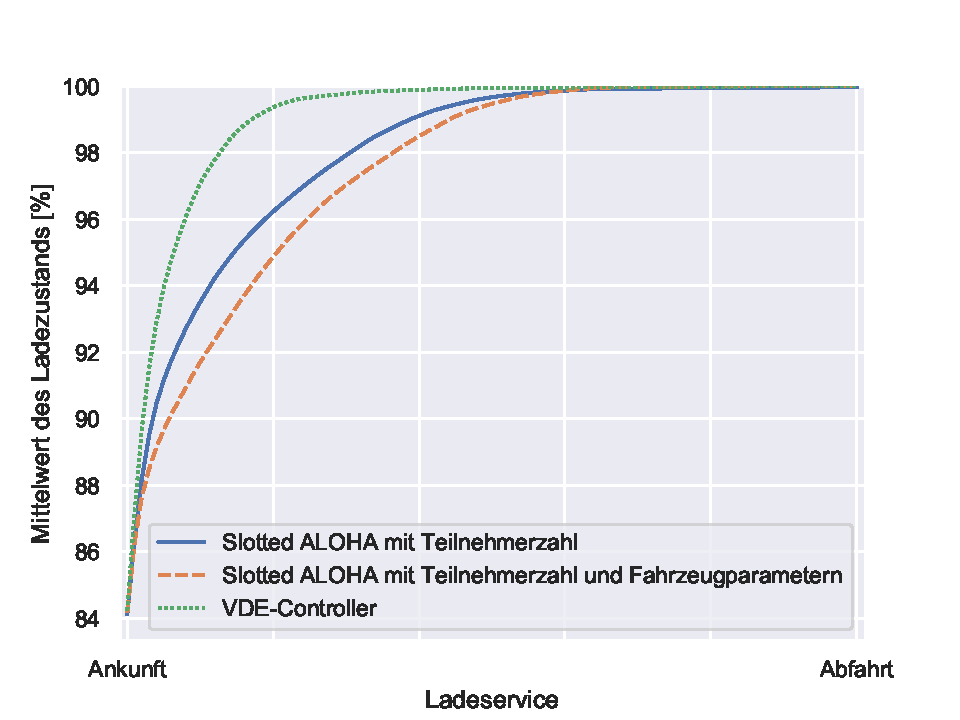
\includegraphics[width=\linewidth]{img/mitTrafo/SlottedAloha_participants_VDE_tau_trafo_15_soc_mean.pdf}
        \subcaption{Durchschnittlicher Ladezustand aller Elektrofahrzeuges über den Verlauf eines Ladeservices}
        \label{ABB_mt_SocMEAN}
	\end{subfigure}
	\begin{subfigure}{0.49\linewidth}
		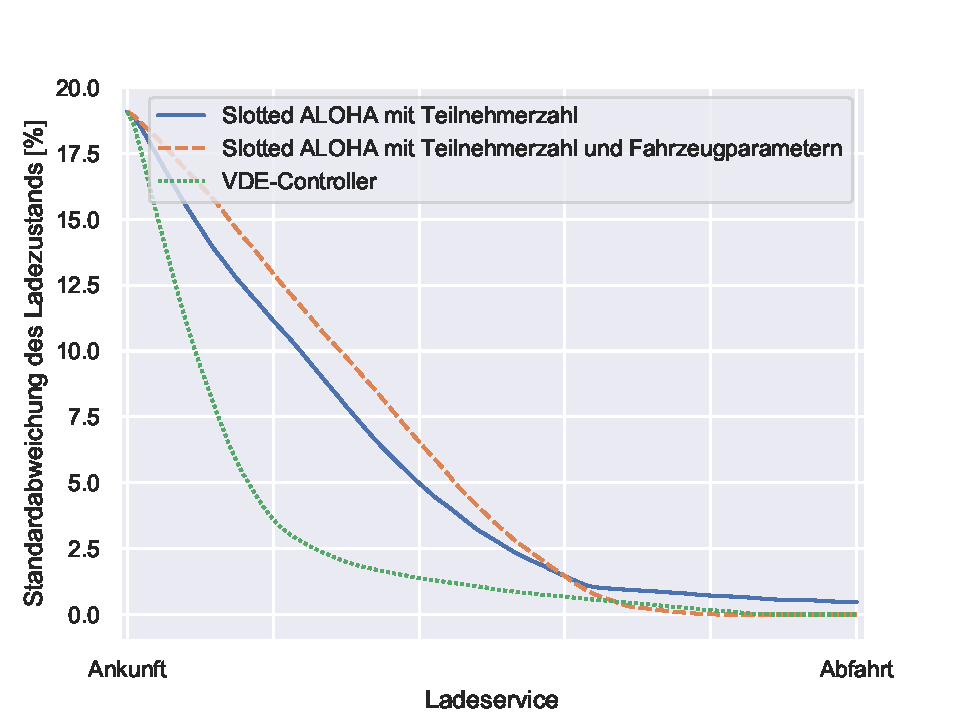
\includegraphics[width=\linewidth]{img/mitTrafo/SlottedAloha_participants_VDE_tau_trafo_15_soc_std.pdf}
        \subcaption{Durschschnittliche Standardabweichung des Ladezustandes aller Elektrofahrzeuges über den Verlauf eines Ladeservices}
        \label{ABB_mT_SocSTD}
	\end{subfigure}
\end{figure}
In Abbildung \ref{ABB_mt_SocMEAN} sind die jeweiligen mittleren Ladestände aller Fahrzeugen über den Verlauf der Ladeservice hinweg dargestellt, Abbildung \ref{ABB_mT_SocSTD} zeigt die zugehörige Standardabweichung. Abbildung \ref{ABB_mT_SocMEAN} zeigt einen ähnlichen Verlauf der Kurven, welche das Netzwerkprotokoll verwenden. Allerdings wird auch ersichtlich, dass die Variante, welche nur die Teilnehmerzahl verwendet, nicht dazu in der Lage ist alle abgeschlossenen Ladeservice auch erfolgreich abzuschließen, da die Standardabweichung nicht bis auf null zurückgeht. Sonst zeigen sich ähnliche Ergebnisse wie beim Vergleich der drei Varianten ohne den Transformatorkontroller.
\begin{figure}[htb]
\centering
	\includegraphics[scale=0.6]{img/mitTrafo/SlottedAloha_participants_VDE_tau_trafo_15_qoe.pdf}
	\caption{Durchschnittlicher Qualitätserfahrung aller Elektrofahrzeuges über den Verlauf eines Ladeservices}
	\label{Abb_mT_Fairness}
\end{figure}
Abbildung \ref{Abb_mT_Fairness} zeigt die mittlere Fairness aller Fahrzeuge über den Verlauf der Ladeservice hinweg mit der zugehörigen Standardabweichung für alle drei betrachteten Varianten. Auch hier zeigt sich wieder der Nachteil der Variante mit dem Netzwerkprotokoll, welche nur die Teilnehmerzahl verwendet, da nicht alle Ladeservice erfolgreich waren, erreicht auch die Fairness nicht dem maximal möglichen Wert. Sonst zeigt der Graph ein ähnliches Ergebnis wie bereits als der Transformatorkontroller noch nicht verwendet wurde.
Insgesamt ergibt sich bei der Betrachtung der Ergebnisse, wenn der Transformatorkontroller verwendet wird dasselbe Bild als, wenn er nicht verwendet wird. Allerdings ist nur bei der Verwendung des Transformatorkontrollers, da das gesetzte Ziel der Regulierung der Transformatorlast erreicht worden, nur die Verwendung eines Spannungskontrollers hat nicht zum Erreichen dieses Ziels ausgereicht.
